\documentclass[a4paper]{article}

\def\npart {II}
\def\nterm {Michaelmas}
\def\nyear {2015}
\def\nlecturer {C.\ Birkar}
\def\ncourse {Galois Theory}

% Imports
\ifx \nextra \undefined
  \usepackage[pdftex,
    hidelinks,
    pdfauthor={Dexter Chua},
    pdfsubject={Cambridge Maths Notes: Part \npart\ - \ncourse},
    pdftitle={Part \npart\ - \ncourse},
  pdfkeywords={Cambridge Mathematics Maths Math \npart\ \nterm\ \nyear\ \ncourse}]{hyperref}
  \title{Part \npart\ - \ncourse}
\else
  \usepackage[pdftex,
    hidelinks,
    pdfauthor={Dexter Chua},
    pdfsubject={Cambridge Maths Notes: Part \npart\ - \ncourse\ (\nextra)},
    pdftitle={Part \npart\ - \ncourse\ (\nextra)},
  pdfkeywords={Cambridge Mathematics Maths Math \npart\ \nterm\ \nyear\ \ncourse\ \nextra}]{hyperref}

  \title{Part \npart\ - \ncourse \\ {\Large \nextra}}
\fi

\author{Lectured by \nlecturer \\\small Notes taken by Dexter Chua}
\date{\nterm\ \nyear}

\usepackage{alltt}
\usepackage{amsfonts}
\usepackage{amsmath}
\usepackage{amssymb}
\usepackage{amsthm}
\usepackage{booktabs}
\usepackage{caption}
\usepackage{enumitem}
\usepackage{fancyhdr}
\usepackage{graphicx}
\usepackage{mathtools}
\usepackage{microtype}
\usepackage{multirow}
\usepackage{pdflscape}
\usepackage{pgfplots}
\usepackage{siunitx}
\usepackage{tabularx}
\usepackage{tikz}
\usepackage{tkz-euclide}
\usepackage[normalem]{ulem}
\usepackage[all]{xy}

\pgfplotsset{compat=1.12}

\pagestyle{fancyplain}
\lhead{\emph{\nouppercase{\leftmark}}}
\ifx \nextra \undefined
  \rhead{
    \ifnum\thepage=1
    \else
      \npart\ \ncourse
    \fi}
\else
  \rhead{
    \ifnum\thepage=1
    \else
      \npart\ \ncourse\ (\nextra)
    \fi}
\fi
\usetikzlibrary{arrows}
\usetikzlibrary{decorations.markings}
\usetikzlibrary{decorations.pathmorphing}
\usetikzlibrary{positioning}
\usetikzlibrary{fadings}
\usetikzlibrary{intersections}
\usetikzlibrary{cd}

\newcommand*{\Cdot}{\raisebox{-0.25ex}{\scalebox{1.5}{$\cdot$}}}
\newcommand {\pd}[2][ ]{
  \ifx #1 { }
    \frac{\partial}{\partial #2}
  \else
    \frac{\partial^{#1}}{\partial #2^{#1}}
  \fi
}

% Theorems
\theoremstyle{definition}
\newtheorem*{aim}{Aim}
\newtheorem*{axiom}{Axiom}
\newtheorem*{claim}{Claim}
\newtheorem*{cor}{Corollary}
\newtheorem*{defi}{Definition}
\newtheorem*{eg}{Example}
\newtheorem*{fact}{Fact}
\newtheorem*{law}{Law}
\newtheorem*{lemma}{Lemma}
\newtheorem*{notation}{Notation}
\newtheorem*{prop}{Proposition}
\newtheorem*{thm}{Theorem}

\renewcommand{\labelitemi}{--}
\renewcommand{\labelitemii}{$\circ$}
\renewcommand{\labelenumi}{(\roman{*})}

\let\stdsection\section
\renewcommand\section{\newpage\stdsection}

% Strike through
\def\st{\bgroup \ULdepth=-.55ex \ULset}

% Maths symbols
\newcommand{\bra}{\langle}
\newcommand{\ket}{\rangle}

\newcommand{\N}{\mathbb{N}}
\newcommand{\Z}{\mathbb{Z}}
\newcommand{\Q}{\mathbb{Q}}
\renewcommand{\H}{\mathbb{H}}
\newcommand{\R}{\mathbb{R}}
\newcommand{\C}{\mathbb{C}}
\newcommand{\Prob}{\mathbb{P}}
\renewcommand{\P}{\mathbb{P}}
\newcommand{\E}{\mathbb{E}}
\newcommand{\F}{\mathbb{F}}
\newcommand{\cU}{\mathcal{U}}
\newcommand{\RP}{\mathbb{RP}}
\newcommand{\CP}{\mathbb{CP}}

\newcommand{\ph}{\,\cdot\,}

\DeclareMathOperator{\sech}{sech}
\DeclareMathOperator{\cosech}{cosech}
\DeclareMathOperator{\cosec}{cosec}

\DeclareMathOperator{\covol}{covol}
\DeclareMathOperator{\vol}{vol}

\let\Im\relax
\let\Re\relax
\DeclareMathOperator{\Im}{Im}
\DeclareMathOperator{\Re}{Re}
\DeclareMathOperator{\im}{im}
\DeclareMathOperator{\image}{image}
\DeclareMathOperator{\Ann}{Ann}

\DeclareMathOperator*{\res}{res}
\DeclareMathOperator{\Res}{Res}
\DeclareMathOperator{\Ind}{Ind}

\DeclareMathOperator{\tr}{tr}
\DeclareMathOperator{\diag}{diag}
\DeclareMathOperator{\rank}{rank}
\DeclareMathOperator{\card}{card}
\DeclareMathOperator{\spn}{span}
\DeclareMathOperator{\adj}{adj}

\DeclareMathOperator{\erf}{erf}
\DeclareMathOperator{\erfc}{erfc}

\DeclareMathOperator{\ord}{ord}
\DeclareMathOperator{\Sym}{Sym}

\DeclareMathOperator{\sgn}{sgn}
\DeclareMathOperator{\orb}{orb}
\DeclareMathOperator{\stab}{stab}
\DeclareMathOperator{\ccl}{ccl}

\DeclareMathOperator{\lcm}{lcm}
\DeclareMathOperator{\hcf}{hcf}

\DeclareMathOperator{\Int}{Int}
\DeclareMathOperator{\id}{id}

\DeclareMathOperator{\betaD}{beta}
\DeclareMathOperator{\gammaD}{gamma}
\DeclareMathOperator{\Poisson}{Poisson}
\DeclareMathOperator{\binomial}{binomial}
\DeclareMathOperator{\multinomial}{multinomial}
\DeclareMathOperator{\Bernoulli}{Bernoulli}
\DeclareMathOperator{\like}{like}

\DeclareMathOperator{\var}{var}
\DeclareMathOperator{\cov}{cov}
\DeclareMathOperator{\bias}{bias}
\DeclareMathOperator{\mse}{mse}
\DeclareMathOperator{\corr}{corr}

\DeclareMathOperator{\otp}{otp}
\DeclareMathOperator{\dom}{dom}

\DeclareMathOperator{\Root}{Root}
\DeclareMathOperator{\supp}{supp}
\DeclareMathOperator{\rel}{rel}
\DeclareMathOperator{\Hom}{Hom}
\DeclareMathOperator{\Aut}{Aut}
\DeclareMathOperator{\Gal}{Gal}
\DeclareMathOperator{\Mat}{Mat}
\DeclareMathOperator{\End}{End}
\DeclareMathOperator{\Char}{char}
\DeclareMathOperator{\ev}{ev}
\DeclareMathOperator{\St}{St}
\DeclareMathOperator{\Lk}{Lk}
\DeclareMathOperator{\disc}{disc}
\DeclareMathOperator{\Isom}{Isom}
\DeclareMathOperator{\length}{length}
\DeclareMathOperator{\energy}{energy}
\DeclareMathOperator{\area}{area}
\DeclareMathOperator{\Syl}{Syl}
\DeclareMathOperator{\cl}{cl}
\DeclareMathOperator{\fix}{fix}

\newcommand{\GL}{\mathrm{GL}}
\newcommand{\SL}{\mathrm{SL}}
\newcommand{\PGL}{\mathrm{PGL}}
\newcommand{\PSL}{\mathrm{PSL}}
\newcommand{\PSU}{\mathrm{PSU}}
\newcommand{\Or}{\mathrm{O}}
\newcommand{\SO}{\mathrm{SO}}
\newcommand{\U}{\mathrm{U}}
\newcommand{\SU}{\mathrm{SU}}

\renewcommand{\d}{\mathrm{d}}
\newcommand{\D}{\mathrm{D}}

\tikzset{->/.style = {decoration={markings,
                                  mark=at position 1 with {\arrow[scale=2]{latex'}}},
                      postaction={decorate}}}
\tikzset{<-/.style = {decoration={markings,
                                  mark=at position 0 with {\arrowreversed[scale=2]{latex'}}},
                      postaction={decorate}}}
\tikzset{<->/.style = {decoration={markings,
                                   mark=at position 0 with {\arrowreversed[scale=2]{latex'}},
                                   mark=at position 1 with {\arrow[scale=2]{latex'}}},
                       postaction={decorate}}}
\tikzset{->-/.style = {decoration={markings,
                                   mark=at position #1 with {\arrow[scale=2]{latex'}}},
                       postaction={decorate}}}
\tikzset{-<-/.style = {decoration={markings,
                                   mark=at position #1 with {\arrowreversed[scale=2]{latex'}}},
                       postaction={decorate}}}

\tikzset{circ/.style = {fill, circle, inner sep = 0, minimum size = 3}}
\tikzset{mstate/.style={circle, draw, blue, text=black, minimum width=0.7cm}}

\definecolor{mblue}{rgb}{0.2, 0.3, 0.8}
\definecolor{morange}{rgb}{1, 0.5, 0}
\definecolor{mgreen}{rgb}{0.1, 0.4, 0.2}
\definecolor{mred}{rgb}{0.5, 0, 0}

\def\drawcirculararc(#1,#2)(#3,#4)(#5,#6){%
    \pgfmathsetmacro\cA{(#1*#1+#2*#2-#3*#3-#4*#4)/2}%
    \pgfmathsetmacro\cB{(#1*#1+#2*#2-#5*#5-#6*#6)/2}%
    \pgfmathsetmacro\cy{(\cB*(#1-#3)-\cA*(#1-#5))/%
                        ((#2-#6)*(#1-#3)-(#2-#4)*(#1-#5))}%
    \pgfmathsetmacro\cx{(\cA-\cy*(#2-#4))/(#1-#3)}%
    \pgfmathsetmacro\cr{sqrt((#1-\cx)*(#1-\cx)+(#2-\cy)*(#2-\cy))}%
    \pgfmathsetmacro\cA{atan2(#2-\cy,#1-\cx)}%
    \pgfmathsetmacro\cB{atan2(#6-\cy,#5-\cx)}%
    \pgfmathparse{\cB<\cA}%
    \ifnum\pgfmathresult=1
        \pgfmathsetmacro\cB{\cB+360}%
    \fi
    \draw (#1,#2) arc (\cA:\cB:\cr);%
}
\newcommand\getCoord[3]{\newdimen{#1}\newdimen{#2}\pgfextractx{#1}{\pgfpointanchor{#3}{center}}\pgfextracty{#2}{\pgfpointanchor{#3}{center}}}

\def\Xint#1{\mathchoice
   {\XXint\displaystyle\textstyle{#1}}%
   {\XXint\textstyle\scriptstyle{#1}}%
   {\XXint\scriptstyle\scriptscriptstyle{#1}}%
   {\XXint\scriptscriptstyle\scriptscriptstyle{#1}}%
   \!\int}
\def\XXint#1#2#3{{\setbox0=\hbox{$#1{#2#3}{\int}$}
     \vcenter{\hbox{$#2#3$}}\kern-.5\wd0}}
\def\ddashint{\Xint=}
\def\dashint{\Xint-}


\begin{document}
\maketitle
{\small
\noindent\emph{Groups, Rings and Modules is essential}
\vspace{10pt}

\noindent Field extensions, tower law, algebraic extensions; irreducible polynomials and relation with simple algebraic extensions. Finite multiplicative subgroups of a field are cyclic. Existence and uniqueness of splitting fields.\hspace*{\fill} [6]

\vspace{5pt}
\noindent Existence and uniqueness of algebraic closure.\hspace*{\fill} [1]

\vspace{5pt}
\noindent Separability. Theorem of primitive element. Trace and norm.\hspace*{\fill} [3]

\vspace{5pt}
\noindent Normal and Galois extensions, automorphic groups. Fundamental theorem of Galois theory.\hspace*{\fill} [3]

\vspace{5pt}
\noindent Galois theory of finite fields. Reduction mod $p$.\hspace*{\fill} [2]

\vspace{5pt}
\noindent Cyclotomic polynomials, Kummer theory, cyclic extensions. Symmetric functions. Galois theory of cubics and quartics.\hspace*{\fill} [4]

\vspace{5pt}
\noindent Solubility by radicals. Insolubility of general quintic equations and other classical problems.\hspace*{\fill} [3]

\vspace{5pt}
\noindent Artin's theorem on the subfield fixed by a finite group of automorphisms. Polynomial invariants of a finite group; examples.\hspace*{\fill} [2]}

\tableofcontents

\setcounter{section}{-1}
\section{Introduction}
The most famous result of Galois theory is that there is no general solution to polynomial equations of degree $5$ or above in terms of radicals. However, this result was, in fact, proven before Galois theory existed, and goes under the name of the \emph{Abel--Ruffini theorem}. What Galois theory does provides is a way to decide whether a given polynomial has a solution in terms of radicals, as well as a nice way to prove this result.

However, Galois theory is more than equation solving. In fact, the \emph{fundamental theorem of Galois theory}, which is obviously an important theorem in Galois theory, has completely nothing to do with equation solving. Instead, it is about group theory.

In modern days, Galois theory is often said to be the study of field extensions. The idea is that we have a field $K$, and then add more elements to get a field $L$. When we want to study solutions to polynomial equations, what we add is the roots of the polynomials. We then study the properties of this field extension, and in some cases, show that this field extension cannot be obtained by just adding radicals.

For certain ``nice'' field extensions $K \subseteq L$, we can assign to it the \emph{Galois group} $\Gal(L/K)$. In general, given any group $G$, we can find subgroups of $G$. On the other hand, given a field extension $K\subseteq L$, we can try to find some intermediate field $F$ that can be fitted into $K \subseteq F \subseteq L$. The key idea of Galois theory is that these two processes are closely related --- we can establish a one-to-one correspondence between the subgroups of $G$ and the intermediate fields $F$.

Moreover, many properties of (intermediate) field extensions correspond to analogous ideas in group theory. For example, we have the notion of normal subgroups, and hence there is an analogous notion of normal extensions. Similarly, we have soluble extensions (i.e.\ extensions that can be obtained by adding radicals), and these correspond to ``soluble groups''. In Galois theory, we will study how group-theoretic notions and field-theoretic notions interact.

Nowadays, Galois theory is an important field in mathematics, and finds its applications in number theory, algebraic geometry and even cryptography.

\section{Solving equations}
Galois theory grew of of the desire to \emph{solve equations}. In particular, to solve polynomial equations. To begin with, we will come up with general solutions to polynomial equations of up to degree $4$. However, this is the best we can do, as we will later show in the course --- there is no general solution to polynomial equations of degree $5$ or above.

Before we start, we will define some notations that we will frequently use.

If $R$ is a ring, then $R[t]$ is the polynomial ring over $R$ in the variable $t$. Usually, we take $R = \Q$ and consider polynomials $f(t) \in \Q[t]$. The objective is then to find roots to the equation $f(t) = 0$. Often, we want to restrict our search domain. For example, we might ask if there is a root in $\Q$. We will thus use $\Root_f(X)$ to denote the set of all roots of $f$ in $X$.

\subsubsection*{Linear equations}
Suppose that $f = t + a \in \Q[t]$ (with $a\in \Q$). This is easy to solve --- we have $\Root_f(\Q) = \{-a\}$.

\subsubsection*{Quadratic equations}
Consider a simple quadratic $f = t^2 + 1 \in \Q[t]$. Then $\Root_f(\Q) = \emptyset$ since the square of all rationals are positive. However, in the complex plane, we have $\Root_f(\C) = \{\sqrt{-1}, -\sqrt{-1}\}$.

In general, let $f = t^2 + at + b\in \Q[t]$. Then as we all know, the roots are given by
\[
  \Root_f(\C) = \left\{\frac{-a \pm \sqrt{a^2 - 4b}}{2}\right\}
\]
\subsubsection*{Cubic equations}
Let $f = t^3 + c\in \Q[t]$. The roots are then
\[
  \Root_f(\C) = \{\sqrt[3]{-c}, \mu\sqrt[3]{-c}, \mu^2 \sqrt[3]{-c}\},
\]
where $\mu = \frac{-1 + \sqrt{-3}}{2}$ is the 3rd root of unity. Note that $\mu$ is defined by the equation $\mu^3 - 1 = 0$, and satisfies $\mu^2 + \mu + 1 = 0$.

In general, let $f = t^3 + at^2 + bt + c \in \Q[t]$, and let $\Root_f(\C) = \{\alpha_1, \alpha_2, \alpha_3\}$, not necessarily distinct.

Our objective is to solve $f = 0$. Before doing so, we have to make it explicit what we mean by ``solving'' the equation. As in solving the quadratic, we want to express the roots $\alpha_1, \alpha_2$ and $\alpha_3$ in terms of ``radicals'' involving $a, b$ and $c$.

Unlike the quadratic case, there is no straightforward means of coming up with a general formula. The result we currently have is the result of many many years of hard work, and the substitutions we make seemingly come out of nowhere. However, after a lot of magic, we will indeed come up with a general formula for it.

We first simplify our polynomial by assuming $a = 0$. Given any polynomial $f = t^3 + at^2 + bt + c$, we know $a$ is the negative of the sum of the roots. So we can increase each root by $\frac{a}{3}$ so that the coefficient of $t^2$ vanishes. So we perform the change of variables $t\mapsto t - \frac{a}{3}$, and get rid of the coefficient of $t^2$. So we can assume $a = 0$.

Let $\mu$ be as above. Define
\begin{align*}
  \beta &= \alpha_1 + \mu \alpha_2 + \mu^2 \alpha_3\\
  \gamma &= \alpha_1 + \mu^2 \alpha_2 + \mu \alpha_3
\end{align*}
These are the \emph{Lagrange resolvers}. We obtain
\begin{align*}
  \beta\gamma &= \alpha_1^2 + \alpha_2^2 +\alpha_3^2 + (\mu + \mu^2)(\alpha_1\alpha_2 + \alpha_2\alpha_3 + \alpha_1\alpha_3)\\
  \intertext{Since $\mu^2 + \mu + 1 = 0$, we have $\mu^2 + \mu = -1$. So we can simplify to obtain}
  &= (\alpha_1 + \alpha_2 + \alpha_3)^2 - 3(\alpha_1\alpha_2 + \alpha_2\alpha_3 + \alpha_1\alpha_3)\\
  \intertext{We have $\alpha_1 + \alpha_2 + \alpha_3 = -a = 0$, while $b = \alpha_1\alpha_2 + \alpha_2\alpha_3 + \alpha_1\alpha_3$. So}
  &= -3b\\
  \intertext{Cubing, we obtain}
  \beta^3\gamma^3 &= -27b^3.
\end{align*}
On the other hand, recalling again that $\alpha_1 + \alpha_2 + \alpha_3 = 0$, we have
\begin{align*}
  \beta^3 + \gamma^3 &= (\alpha_1 + \mu \alpha_2 + \mu^2 \alpha_3)^3 + (\alpha_1 + \mu^2\alpha_2 + \mu \alpha_3)^3 + (\alpha_1 + \alpha_2 + \alpha_3)^3\\
  &= 3(\alpha_1^2 + \alpha_2^3 + \alpha_3^2) + 18\alpha_1\alpha_2\alpha_3\\
  \intertext{We have $\alpha_1\alpha_2\alpha_3 = -c$, and since $\alpha_i^3 + b\alpha_i + c = 0$ for all $i$, summing gives $\alpha_1^3 + \alpha_2^3 + \alpha_3^3 + 3c = 0$. So}
  &= -27c
\end{align*}
Hence, we obtain
\[
  (t - \beta^3)(t - \gamma^3) = t^2 + 27ct - 27b^3.
\]
We already know how to solve this equation using the quadratic formula. We obtain
\[
  \{\beta^3, \gamma^3\} = \left\{\frac{-27 c \pm \sqrt{(27c)^2 + 4\times 27b^3}}{2}\right\}
\]
We now have $\beta^3$ and $\gamma^3$ in terms of radicals. So we can find $\beta$ and $\gamma$ in terms of radicals. Finally, we can solve for $\alpha_i$ using
\begin{align*}
  0 &= \alpha_1 + \alpha_2 + \alpha_3\\
  \beta &= \alpha_1 + \mu \alpha_2 + \mu^2 \alpha_3\\
  \gamma &= \alpha_1 + \mu^2 \alpha_2 + \mu \alpha_3
\end{align*}
In particular, we obtain
\begin{align*}
  \alpha_1 &= \frac{1}{3}(\beta + \gamma)\\
  \alpha_2 &= \frac{1}{3}(\mu^2 \beta + \mu \gamma)\\
  \alpha_3 &= \frac{1}{3}(\mu \beta + \mu^2 \gamma)
\end{align*}
So we can solve a cubic in terms of radicals.

This was a lot of magic involved, and indeed this was discovered through a lot of hard work throughout many many years. This is also not a very helpful result since we have no idea where these substitutions came from and why they intuitively work.

\subsubsection*{Quartic equations}
Assume $f = t^4 + at^3 + bt^2 + ct + d\in \Q[t]$. Let $\Root_f(\C) = \{\alpha_1, \alpha_2, \alpha_3, \alpha_4\}$. Can we express all these in terms of radicals? Again the answer is yes, but the procedure is much more complicated.

We can perform a similar change of variable to assume $a = 0$. So $\alpha_1 + \alpha_2 + \alpha_3 + \alpha_4 = 0$.

This time, define
\begin{align*}
  \beta &= \alpha_1 + \alpha_2\\
  \gamma &= \alpha_1 + \alpha_3\\
  \lambda &= \alpha_1 + \alpha_4
\end{align*}
Doing some calculations, we see that
\begin{align*}
  \beta^2 &= -(\alpha_1 + \alpha_2)(\alpha_3 + \alpha_4)\\
  \gamma^2 &= -(\alpha_1 + \alpha_3)(\alpha_2 + \alpha_4)\\
  \lambda^2 &= -(\alpha_1 + \alpha_4)(\alpha_2 + \alpha_3)
\end{align*}
Now consider
\begin{align*}
  g &= (t - \beta^2)(t - \gamma^2)(t - \lambda^2)\\
  &= t^3 + 2bt^2 + (b^2 - 4d)t - c^2
\end{align*}
This we know how to solve, and so we are done.

\subsubsection*{Quintics and above}
So far so good. But how about polynomials of higher degrees? In general, let $f \in \Q[t]$. Can we write down all the roots of $f$ in terms of radicals? We know that the answer is yes if $\deg f \leq 4$.

Unfortunately, for $\deg f \geq 5$, the answer is no. Of course, this ``no'' means no \emph{in general}. For example, $f = (t - 1)(t - 2) \cdots (t - 5)\in \Q[t]$ has the obvious roots in terms of radicals.

There isn't an easy proof of this result. The general idea is to first associate a \emph{field extension} $F \supseteq \Q$ for our polynomial $f$. This field $F$ will be obtained by adding all roots of $f$. Then we associate a \emph{Galois group} $G$ to this field extension. We will then prove a theorem that says $f$ has a solution in terms of radicals if and only if the Galois group is ``soluble'', where ``soluble'' has a specific algebraic definition in group theory we will explore later. Finally, we find specific polynomials whose Galois group is not soluble.

\section{Field extensions}
After all that (hopefully) fun introduction and motivation, we will now start Galois theory in a more abstract way. The modern approach is to describe these in terms of field extensions.

\subsection{Field extensions}
\begin{defi}[Field extension]\index{field extension}\index{subfield}
  A \emph{field extension} is an inclusion of a field $K\subseteq L$, where $K$ inherits the algebraic operations from $L$. We also write this as \term{$L/K$}. Alternatively, we can define this by a injective homomorphism $K\to L$. We say $L$ is an \emph{extension} of $K$, and $K$ is a \emph{subfield} of $L$.
\end{defi}

\begin{eg}\leavevmode
  \begin{enumerate}
    \item $\R/\Q$ is a field extension.
    \item $\C\Q$ is a field extension.
    \item $\Q(\sqrt{2}) = \{a + b\sqrt{2}: a, b\in \Q\} \subseteq \R$ is a field extension over $\Q$.
  \end{enumerate}
\end{eg}

Given a field extension $L/K$, we want to quantify how much ``bigger'' $L$ is compared to $K$. For example, to get from $\Q$ to $\R$, we need to add a lot of elements (since $\Q$ is countable and $\R$ is uncountable). On the other hand, to get from $\R$ to $\C$, we just need to add a single element $\sqrt{-1}$.

To do so, we can consider $L$ as a vector space over $K$. We know that $L$ already comes with an additive abelian group structure, and we can define scalar multiplication by simply multiplying: if $a\in K, \alpha\in L$, then $a\cdot \alpha$ is defined as multiplication in $L$.

\begin{defi}[Degree of field extension]\index{degree}
  The \emph{degree} of $L$ over $K$ is $[L:K]$ is the dimension of $L$ as a vector space over $K$. The extension is \emph{finite} if the degree is finite.
\end{defi}
In this course, we are mostly concerned with finite extensions.

\begin{eg}\leavevmode
  \begin{enumerate}
    \item Consider $\C/\R$. This is a finite extension with degree $[\C:\R] = 2$ since we have a basis of $\{1, i\}$.
    \item The extension $\Q(\sqrt{2})/\Q$ has degree $2$ since we have a basis of $\{1, \sqrt{2}\}$.
    \item The extension $\R/\Q$ is not finite.
  \end{enumerate}
\end{eg}

We are going to use the following result a lot:
\begin{thm}[Tower Law]
  Let $F/L/K$ be field extensions. Then
  \[
    [F:K] = [F:L][L:K]
  \]
\end{thm}

\begin{proof}
  Assume $[F:L]$ and $[L:K]$ are finite. Let $\{\alpha_1, \cdots, \alpha_m\}$ be a basis for $L$ over $K$, and $\{\beta_1, \cdots, \beta_n\}$ be a basis for $F$ over $L$. Pick $\gamma \in F$. Then we can write
  \[
    \gamma = \sum_i b_i \beta_i,\quad b_i\in L.
  \]
  For each $b_i$, we can write as
  \[
    b_i = \sum_j a_{ij}\alpha_{j},\quad a_{ij}\in K.
  \]
  So we can write
  \[
    \gamma = \sum_i \left(\sum_j a_{ij}\alpha_j\right)\beta_i = \sum_{i, j} a_{ij}\alpha_j \beta_i.
  \]
  So $T = \{\alpha_j\beta_i\}_{i, j}$ spans $F$ over $K$. To show that this is a basis, we have to show that they are linearly independent. Consider the case where $\gamma = 0$. Then we must have $b_i = 0$ since $\{\beta_i\}$ is a basis of $F$ over $L$. Hence each $a_{ij} = 0$ since $\{\alpha_j\}$ is a basis of $L$ over $K$.

  This implies that $T$ is a basis of $F$ over $K$. So
  \[
    [F:K] = |T| = nm = [F:L][L:K].
  \]
  Finally, if $[F:L] = \infty$ or $[L:K] = \infty$, then clearly $[F:K] = \infty$ as well. So equality holds as well.
\end{proof}

Recall that in IA Numbers and Sets, we defined a real number $x$ to be algebraic if it is a root of some polynomial in integer (or rational) coefficients. We can do this for general field (extensions) as well.
\begin{defi}[Algebraic number]
  Let $L/K$ be a field extension, $\alpha\in L$. We define
  \[
    I_\alpha = \{f\in K[t] : f(\alpha) = 0\}\subseteq K[t]
  \]
  This is the set of polynomials for which $\alpha$ is a root. It is easy to show that $I_\alpha$ is an ideal, since it is the kernel of the ring homomorphism $K[t] \to L$ by $g \mapsto g(\alpha)$.

  We say $\alpha$ is \emph{algebraic} over $K$ if $I_\alpha \not= 0$. Otherwise, $\alpha$ is \emph{transcendental} over $K$.

  We say $L$ is \emph{algebraic} over $K$ if every element of $L$ is algebraic.
\end{defi}

\begin{eg}\leavevmode
  \begin{enumerate}
    \item $\sqrt[9]{7}$ is algebraic over $\Q$ because $f(\sqrt[9]{7}) = 0$, where $f = t^9 - 7$. In general, any number written with radicals is algebraic over $\Q$.
    \item $\pi$ is not algebraic over $\Q$.
  \end{enumerate}
\end{eg}
These are rather simple examples, and the following lemma will provide us a way of generating much more examples.

\begin{lemma}
  Let $L/K$ be a finite extension. Then $L$ is algebraic over $K$.
\end{lemma}

\begin{proof}
  Let $n = [L:K]$, and let $\alpha\in L$. Then $1, \alpha, \alpha^2, \cdots, \alpha^n$ are linearly dependent over $K$ (since there are $n + 1$ elements). So there exists some $a_i \in K$ (not all zero) such that
  \[
    a_n \alpha^n + a_{n - 1}\alpha^{n - 1} + \cdots + a_1 \alpha + a_0 = 0.
  \]
  So we have a non-trivial polynomial that vanishes at $\alpha$. So $\alpha$ is algebraic over $K$.

  Since $\alpha$ was arbitrary, $L$ itself is algebraic.
\end{proof}

If $L/K$ is a field extension and $\alpha \in L$ is algebraic, then by definition, there is some polynomial $f$ such that $f(\alpha) = 0$. It is a natural question to ask if there is a ``smallest'' polynomial that does this job. Obviously we can find a polynomial of smallest \emph{degree} (by the well-ordering principle of the natural numbers), but we can get something even stronger.

Since $K$ is a field, $K[t]$ is a PID (principal ideal domain). This, by definition, implies we can find some (monic) $P_\alpha \in K[t]$ such that $I_\alpha = \bra P_\alpha\ket$. In other words, every element of $I_\alpha$ is just a multiple of $P_\alpha$.
\begin{defi}[Minimal polynomial]
  Let $L/K$ be a field extension, $\alpha \in L$. The \emph{minimal polynomial} of $\alpha$ over $K$ is a monic polynomial $P_\alpha$ such that $I_\alpha = \bra P_\alpha\ket$.
\end{defi}

\begin{eg}\leavevmode
  \begin{enumerate}
    \item Consider $\R/\Q$, $\alpha = \sqrt[3]{2}$. Then the minimal polynomial is $P_\alpha = t^3 - 2$.
    \item Consider $\C/\R$, $\alpha = \sqrt[3]{2}$. Then the minimal polynomial is $P_\alpha = t - \sqrt[3]{2}$.
  \end{enumerate}
\end{eg}

It should be intuitively obvious that by virtue of being ``minimal'', the minimal polynomial is irreducible.
\begin{prop}
  Let $L/K$ be a field extension, $\alpha\in L$ algebraic over $K$, and $P_\alpha$ the minimal polynomial. Then $P_\alpha$ is irreducible in $K[t]$.
\end{prop}

\begin{proof}
  Assume that $P_\alpha = QR$ in $K[t]$. So $0 = P_\alpha(\alpha) = Q(\alpha) R(\alpha)$. So $Q(\alpha) = 0$ or $R(\alpha) = 0$. Say $Q(\alpha) = 0$. So $Q\in I_\alpha$. So $Q$ is a multiple of $P_\alpha$. However, we also know that $P_\alpha$ is a multiple of $Q_\alpha$. This is possible only if $R$ is a unit in $K[t]$, i.e.\ $R\in K$. So $P_\alpha$ is irreducible.
\end{proof}
It should also be clear that if $f$ is irreducible and $f(\alpha) = 0$, then $f$ is the minimal polynomial. Often, it is the irreducibility of $P_\alpha$ that is important.

Apart from the minimal polynomial, we can also ask for the minimal field containing $\alpha$.
\begin{defi}[Field generated by $\alpha$]
  Let $L/K$ be a field extension, $\alpha\in L$. We define $K(\alpha)$ to be the smallest subfield of $L$ containing $K$ and $\alpha$. We call $K(\alpha)$ the \emph{field generated by $\alpha$ over $K$}.
\end{defi}
This definition by itself is rather abstract and not very helpful. Intuitively, $K(\alpha)$ is what we get when we add $\alpha$ to $K$, plus all the extra elements needed to make $K(\alpha)$ a field (i.e.\ closed under addition, multiplication and inverse). We can express this idea more formally by the following result:

\begin{thm}
  Let $L/K$ a field extension, $\alpha\in L$ algebraic. Then
  \begin{enumerate}
    \item $K(\alpha)$ is the image of the (ring) homomorphism $\phi: K[t] \to L$ defined by $f \mapsto f(\alpha)$.
    \item $[K(\alpha): K] = \deg P_\alpha$, where $P_\alpha$ is the minimal polynomial of $\alpha$ over $K$.
  \end{enumerate}
\end{thm}
Note that the kernel of the homomorphism $\phi$ is (almost) by definition the ideal $\bra P_\alpha\ket$. So this theorem tells us
\[
  \frac{K[t]}{\bra P_\alpha\ket}\cong K(\alpha).
\]
\begin{proof}\leavevmode
  \begin{enumerate}
    \item Let $F$ be the image of $\phi$. The first step is to show that $F$ is indeed a field. Since $F$ is the image of a ring homomorphism, we know $F$ is a subring of $L$. Given $\beta \in F$ non-zero, we have to find an inverse.

      By definition, $\beta = f(\alpha)$ for some $f\in K[t]$. The idea is to use B\'ezout's identity. Since $\beta \not= 0$, $f(\alpha) \not= 0$. So $f \not \in I_\alpha = \bra P_\alpha\ket$. So $P_\alpha \nmid f$ in $K[t]$. Since $P_\alpha$ is irreducible, $P_\alpha$ and $f$ are coprime. Then there exists some $g, h \in K[t]$ such that $fg + hP_\alpha = 1$. So $f(\alpha)g(\alpha) = f(\alpha) g(\alpha) + h(\alpha)P_\alpha(\alpha) = 1$. So $\beta g(\alpha) = 1$. So $\beta$ has an inverse. So $F$ is a field.

      From the definition of $F$, we have $K \subseteq F$ and $\alpha \in F$, using the constant polynomials $f = c \in K$ and the identity $f = t$.

      Now, if $K\subseteq G\subseteq L$ and $\alpha \in G$, then $G$ contains all the polynomial expressions of $\alpha$. Hence $F\subseteq G$. So $K(\alpha) = F$.
    \item Let $n = \deg P_\alpha$. We show that $\{1, \alpha, \alpha^2, \cdots, \alpha^{n - 1}\}$ is a basis for $K(\alpha)$ over $K$.

      First note that since $\deg P_\alpha = n$, we can write
      \[
        \alpha^n = \sum_{i = 0}^{n - 1} a_i \alpha^i.
      \]
      So any other higher powers are also linear combinations of the $\alpha^i$s (by induction). This means that $K(\alpha)$ is spanned by $1, \cdots, \alpha^{n - 1}$ as a $K$ vector space.

      It remains to show that $\{1, \cdots, \alpha^{n - 1}\}$ is linearly independent. Assume not. Then for some $b_i$, we have
      \[
        \sum_{i = 0}^{n - 1} b_i \alpha^i = 0.
      \]
      Let $f = \sum b_i t^i$. Then $f(\alpha) = 0$. So $f \in I_\alpha = \bra P_\alpha\ket$. However, $\deg f < \deg P_\alpha$. So we must have $f = 0$. So all $b_i = 0$. So $\{1, \cdots, \alpha^{n - 1}\}$ is a basis for $K(\alpha)$ over $K$. So $[K(\alpha): K] = n$.
  \end{enumerate}
\end{proof}

\begin{cor}
  Let $L/K$ be a field extension, $\alpha \in L$. Then $\alpha$ is algebraic over $K$ if and only if $K \subseteq K(\alpha)$ is a finite extension.
\end{cor}

\begin{proof}
  If $\alpha$ is algebraic, then $[K(\alpha): K] = \deg P_\alpha < \infty$ by above. So the extension is finite.

  If $K\subseteq K(\alpha)$ is a finite extension, then by previous lemma, the entire $K(\alpha)$ is algebraic over $K$. So $\alpha$ is algebraic over $K$.
\end{proof}

We can extend this definition to allow more elements in the generating set.
\begin{defi}[Field generated by elements]
  Let $L/K$ be a field extension, $\alpha_1, \cdots, \alpha_n\subseteq L$. We define $K(\alpha_1, \cdots, \alpha_n)$ to be the smallest subfield of $L$ containing $K$ and $\alpha_1, \cdots, \alpha_n$.

  We call $K(\alpha_1, \cdots, \alpha_n)$ the \emph{field generated by} $\alpha_1, \cdots, \alpha_n$ over $K$.
\end{defi}

And we can prove some similar results.

\begin{thm}
  Suppose that $L/K$ is a field extension.
  \begin{enumerate}
    \item If $\alpha_1, \cdots, \alpha_n \in L$ are algebraic over $K$, then $K\subseteq K(\alpha_1, \cdots, \alpha_n)$ is a finite extension.
    \item If we have $K\subseteq F\subseteq L$ and $K\subseteq F$ is a finite extension, then $F = K(\alpha_1, \cdots, \alpha_n)$ for some $\alpha_1,\cdots, \alpha_n \in L$.
  \end{enumerate}
\end{thm}

\begin{proof}\leavevmode
  \begin{enumerate}
    \item We prove this by induction. Since $\alpha_1$ is algebraic over $K$, $K\subseteq K(\alpha_1)$ is a finite extension.

      For $1 \leq i < n$, $\alpha_{i + 1}$ is algebraic over $K$. So $\alpha_{i + 1}$ is also algebraic over $K(\alpha_1, \cdots, \alpha_i)$. So $K(\alpha_1, \cdots, \alpha_i)\subseteq K(\alpha_1, \cdots, \alpha_i)(\alpha_{i + 1})$ is a finite extension. But $K(\alpha_1, \cdots, \alpha_i)(\alpha_{i + 1}) = K(\alpha_1, \cdots, \alpha_{i + 1})$. By the tower law, $K \subseteq K(\alpha_i, \cdots, \alpha_{i + 1})$ is a finite extension.

    \item Since $F$ is a finite dimensional vector space over $K$, we can take a basis $\{\alpha_1, \cdots, \alpha_n\}$ of $F$ over $K$. Then it should be clear that $F = K(\alpha_1, \cdots, \alpha_n)$.
  \end{enumerate}
\end{proof}

When studying polynomials, the following result from IB Groups, Rings and Modules is often helpful:
\begin{prop}[Eisenstein's criterion]
  Let $f = a_nt^n + \cdots + a_1 t + a_0\in \Z[t]$. Assume that there is some prime number $p$ such that
  \begin{enumerate}
    \item $ p \mid a_i$ for all $i < n$.
    \item $p \nmid a_n$
    \item $p^2 \nmid a_0$.
  \end{enumerate}
  Then $f$ is irreducible in $\Q[t]$.
\end{prop}

\begin{eg}
  Consider the field extensions
  \[
    \Q \subseteq \Q(\sqrt{2})\subseteq \Q(\sqrt{2}, \sqrt[3]{2})\subseteq \R,
  \]
  \[
    \Q\subseteq \Q(\sqrt[3]{2}) \subseteq \Q(\sqrt{2}, \sqrt[3]{2})\subseteq \R.
  \]
  We have $[\Q(\sqrt{2}): \Q] = 2$ since $\{1, \sqrt{2}\}$ is a basis of $\Q(\sqrt{2})$ over $\Q$.

  How about $[\Q(\sqrt[3]{2}):\Q]$? By the Eisenstein criterion, we know that $t^3 - 2$ is irreducible in $\Q[t]$. So the minimal polynomial of $\sqrt[3]{2}$ over $\Q$ is $t^3 - 2$ which has degree 3. So $[\Q(\sqrt[3]{2}):\Q] = 3$.

  These results immediately tells that $\sqrt[3]{2}\not\in \Q(\sqrt{2})$. Otherwise, this entails that $\Q(\sqrt[3]{2}) \subseteq \Q(\sqrt{2})$. Then the tower law says that
  \[
    [\Q(\sqrt{2}):\Q] = [\Q(\sqrt{2}):\Q(\sqrt[3]{2})][\Q(\sqrt[3]{2}):\Q].
  \]
  In particular, plugging the numbers in entails that that $3$ is a factor of $2$, which is clearly nonsense. Similarly, $\sqrt{2}\not \in \Q(\sqrt[3]{2})$.

  How about the inclusion $\Q(\sqrt{2})\subseteq \Q(\sqrt{2}, \sqrt[3]{2})$? We now show that the minimal polynomial $P_{\sqrt[3]{2}}$ of $\sqrt[3]{2}$ over $\Q(\sqrt{2})$ is $t^3 - 2$.

  Suppose not. Then $t^3 - 2$ is reducible, with the real $P_{\sqrt[3]{2}}$ as one of its factors. Let $t^3 - 2 = P_{\sqrt[3]{2}} \cdot R$ for some non-unit polynomial $R$.

  We know that $P_{\sqrt[3]{2}}$ does not have degree 3 (or else it would be $t^3 - 2$), and not degree 1, since a degree 1 polynomial has a root. So it has degree $2$. So $R$ has degree $1$. Then $R$ has a root, i.e.\ $R(\beta) = 0$ for some $\beta \in \Q(\sqrt{2})$. So $\beta^3 - 2 = 0$. Hence $[\Q(\beta): \Q] = 3$. Again, by the tower law, we have
  \[
    [\Q(\sqrt{2}):\Q] = [\Q(\sqrt{2}):\Q(\beta)][\Q(\beta):\Q].
  \]
  Again, this is nonsense since it entails that 3 is a factor of 2. So the minimal polynomial is indeed $t^3 -2$. So $[\Q(\sqrt{2}, \sqrt[3]{2}):\Q] = 6$ by the tower law.

  Alternatively, we can obtain this result by noting that the tower law on $\Q \subseteq \Q(\sqrt{2})\subseteq \Q(\sqrt{2}, \sqrt[3]{2})$ and $\Q\subseteq \Q(\sqrt[3]{2}) \subseteq \Q(\sqrt{2}, \sqrt[3]{2})$ entails that 2 and 3 are both factors of $[\Q(\sqrt{2}, \sqrt[3]{2}):\Q]$. So it is at least $6$. Then since $t^3 - 2\in \Q(\sqrt{2})[t]$ has $\sqrt[3]{2}$ as a root, the degree is at most 6. So it is indeed 6.
\end{eg}
\subsection{Ruler and compass constructions}
Before we develop our theory further, we first look into a rather unexpected application of field extensions. We are going to look at some classic problems in geometry, and solve them using what we've learnt so far. In particular, we want to show that certain things cannot be constructed using a compass and a ruler (as usual, we assume the ruler does not have markings on it).

It is often easy to prove that certain things are constructible --- just exhibit an explicit construction of it. However, it is much more difficult to show that things are \emph{not} constructible. Two classical examples are
\begin{enumerate}
  \item Doubling the cube: Given a cube, can we construct the side of another cube whose volume is double the volume of the original cube?
  \item Trisecting an angle: Given an angle, can we divide the angle into three equal angles?
\end{enumerate}
The idea here is to associate with each possible construction a field extension, and then prove certain results about how these field extensions should behave. We then show that if we could, say, double the cube, then this construction would inevitable break some of the properties it should have.

Firstly, we want to formulate our problem in a more convenient way. In particular, we will view the plane as $\R^2$, and describe lines and circles by equations. We also want to describe ``compass and ruler'' constructions in a more solid way.
\begin{defi}[Constructible points]
  Let $S\subseteq \R^2$ be a set of (usually finite) points in the plane.

  A ``ruler'' allows us to do the following: if $P, Q\in S$, then we can draw the line passing through $P$ and $Q$.

  A ``compass'' allows us to do the following: if $P, Q, Q'\in S$, then we can draw the circle with center at $P$ and radius of length $QQ'$.

  Any point $R\in \R^2$ is \emph{1-step constructible} from $S$ if $R$ belongs to the intersection of two distinct lines or circles constructed from $S$ using rulers and compasses.

  A point $R\in \R^2$ is \emph{constructible} from $S$ if there is some $R_1, \cdots, R_n = R \in \R^2$ such that $R_{i + 1}$ is 1-step constructible from $S\cup \{R_1, \cdots, R_i\}$ for each $i$.
\end{defi}

\begin{eg}
  Let $S = \{(0, 0), (1, 0)\}$. What can we construct? It should be easy to see that $(n, 0)$ for all $n \in \Z$ are all constructible from $S$. In fact, we can show that all points of the form $(m, n)\in \Z$ are constructible from $S$.
  \begin{center}
    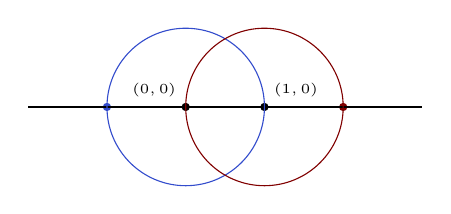
\begin{tikzpicture}
      \node [circ] at (0, 0) {};
      \node [anchor = south east] at (0, 0) {\tiny $(0, 0)$};
      \node [circ] at (1, 0) {};
      \node [anchor = south west] at (1, 0) {\tiny $(1, 0)$};
      \node [mblue] [circ] at (-1, 0) {};
      \node [mred] [circ] at (2, 0) {};

      \draw (-2, 0) -- (3, 0);
      \draw [mblue] circle [radius=1];
      \draw [mred] (1, 0) circle [radius = 1];
    \end{tikzpicture}
  \end{center}
\end{eg}

\begin{defi}[Field of $S$]
  Let $S\subseteq \R^2$ be finite. Define the \emph{field of} $S$ by
  \[
    \Q(S) = \Q(\{\text{coordinates of points in }S\}) \subseteq \R,
  \]
  where we put in the $x$ coordinate and $y$ coordinate separately into the generating set.
\end{defi}
For example, if $S = \{(\sqrt{2}, \sqrt{3})\}$, then $\Q(S) = \Q(\sqrt{2}, \sqrt{3})$.

The key theorem we will use to prove our results is
\begin{thm}
  Let $S\subseteq \R^2$ be finite. Then
  \begin{enumerate}
    \item If $R$ is 1-step constructible from $S$, then $[\Q(S\cup \{R\}):\Q(S)] = 1$ or $2$.
    \item If $T\subseteq \R^2$ is finite, $S\subseteq T$, and the points in $T$ are constructible from $S$, Then $[\Q(S\cup T): \Q(S)] = 2^k$ for some $k$ (where $k$ can be $0$).
  \end{enumerate}
\end{thm}

\begin{proof}
  By assumption, there are distinct lines or circles $C, C'$ constructed from $S$ using ruler and compass, such that $R\in C\cap C'$. By elementary geometry, $C$ and $C'$ can be given by the equations
  \begin{align*}
    C&: a(x^2 + y^2) + bx + cy + d = 0,\\
    C'&: a'(x^2 + y^2) + b'x + c'y + d' = 0.
  \end{align*}
  where $a, b, c, d, a', b', c', d' \in \Q(S)$. In particular, if we have a line, then we can take $a = 0$.

  Let $R = (r_1, r_2)$. If $a = a' = 0$ (i.e.\ $C$ and $C'$ are lines), then solving the two linear equations gives $r_1, r_2 \in \Q(S)$. So $[\Q(S\cup \{R\}):\Q(S)] = 1$.

  So we can now assume wlog that $a\not = 0$. We let
  \[
    p = a'b - ab',\quad q = a'c - ac',\quad \ell = a'd - ad',
  \]
  which are the coefficients when we perform $a'\times C - a \times C'$. Then by assumption, $p \not= 0$ or $q \not= 0$. Otherwise, $c$ and $c'$ would be the same curve. wlog $p \not= 0$. Then since $(r_1, r_2)$ satisfy both equations of $C$ and $C'$, they satisfy
  \[
    px + qy + \ell = 0.
  \]
  In other words, $pr_1 + qr_2 + \ell = 0$. This tells us that
  \[
    r_1 = -\frac{qr_2 + \ell}{p}.\tag{$*$}
  \]
  If we put $r_1, r_2$ into the equations of $C$ and $C'$ and use $(*)$, we get an equation of the form
  \[
    \alpha r_2^2 + \beta r_2 + \gamma = 0,
  \]
  where $\alpha, \beta, \gamma \in \Q(S)$. So we can find $r_2$ (and hence $r_1$ using linear relations) using only a single radical of degree 2. So
  \[
    [\Q(S\cup \{R\}):\Q(S)] = [\Q(S)(r_2): \Q(S)] = 1\text{ or }2,
  \]
  since the minimal polynomial of $r_2$ over $\Q(S)$ has degree 1 or 2.

  Then (ii) follows directly from induction, using the tower law.
\end{proof}

\begin{cor}
  It is impossible to ``double the cube''.
\end{cor}

\begin{proof}
  Consider the cube with unit side length, i.e.\ we are given the set $S = \{(0, 0), (1, 0)\}$. Then doubling the cube would correspond to constructing a side of length $\ell$ such that $\ell^3 = 2$, i.e.\ $\ell = \sqrt[3]{2}$. Thus we need to construct a point $R = (\sqrt[3]{2}, 0)$ from $S$.

  If we can indeed construct this $R$, then we need
  \[
    [\Q(S\cup \{R\}):\Q(S)] = 2^k
  \]
  for some $k$. But we know that $\Q(S) = \Q$ and $\Q(S\cup \{R\}) = \Q(\sqrt[3]{2})$, and that
  \[
    [\Q(\sqrt[3]{2}):\Q] = 3.
  \]
  This is a contradiction since $3$ is not a power of $2$.
\end{proof}

\subsection{\texorpdfstring{$K$}{K}-homomorphisms and the Galois Group}
Usually in mathematics, we not only want to study objects, but maps between objects. Suppose we have two field extensions $K \subseteq L$ and $K \subseteq L'$. What should a map between these two objects look like? Obviously, we would like this map to be a field homomorphisms between $L$ and $L'$. Moreover, since this is a map between the two field \emph{extensions}, and not just the fields themselves, we would like this map to preserve things in $K$, and is just a map between the ``extended parts'' of $L$ and $L'$.

\begin{defi}[$K$-homomorphism]
  Let $L/K$ and $L'/K$ be field extensions. A $K$-\emph{homomorphism} $\phi: L \to L'$ is a ring homomorphism such that $\phi|_K = \id$, i.e.\ it fixes everything in $K$. We write $\Hom_K(L, L')$ for the set of all $K$-homomorphisms $L\to L'$.

  A $K$-\emph{isomorphism} is a $K$-homomorphism which is an isomorphism of rings. A $K$-\emph{automorphism} is a $K$-isomorphism $L\to L$. We write $\Aut_K(L)$ for the set of all $K$-automorphism $L\to L$.
\end{defi}
There are a couple of things to take note of
\begin{enumerate}
  \item Given any $\phi \in \Hom_K(L, L')$, we know that
    \begin{enumerate}
      \item Since $\phi|_K = \id$, we know that $\ker \phi \not= L$. Since we know that $\ker \phi$ is an ideal, and a field only has two ideals, we must have $\ker \phi = 0$. So $\phi$ is injective. It is, in fact, true that any homomorphisms of fields is injective.
      \item $\phi$ gives an isomorphism $L \to \phi(L)$. So $\phi(L)$ is a field and we get the field extensions $K\subseteq \phi(L) \subseteq L'$.
    \end{enumerate}
  \item If $[L:K] = [L':K] < \infty$, then any homomorphism in $\Hom_K(L, L')$ is in fact an isomorphism. So
    \[
      \{K\text{-homomorphisms}: L \to L'\} = \{K\text{-isomorphisms}: L\to L'\},
    \]
    This is since any $K$-homomorphism $\phi: L\to L'$ is an injection. So $[L:K] = [\phi(L):K]$. Hence we know that $[L':K] = [\phi(L):K]$. But we know that $\phi(L)$ is a subfield of $L'$. This is possible only if $L' = \phi(L)$. So $\phi$ is a surjection, and hence an isomorphism.

    In particular, $\Aut_K(L) = \Hom_K(L, L)$.
\end{enumerate}

\begin{eg}
  We want to determine $\Aut_\R(\C)$. If we pick any $\psi\in \Aut_\R(\C)$, then
  \[
    (\psi(\sqrt{-1}))^2 + 1 = \psi(\sqrt{-1}^2 + 1) = \psi(0) = 0.
  \]
  So under any automorphism $\psi$, the image of $\sqrt{-1}$ is a root of $t^2 + 1$. Therefore $\psi(\sqrt{-1}) = \sqrt{-1}$ or $-\sqrt{-1}$. In the first case, $\psi$ is the identity. In the second case, the automorphism is $\phi: a + b\sqrt{-1} \mapsto a - b\sqrt{-1}$, i.e.\ the complex conjugate. So $\Aut_\R(\C) = \{\id, \phi\}$.

  Similarly, we can show that $\Aut_\Q(\Q(\sqrt{2})) = \{\id, \phi\}$, where $\phi$ swaps $\sqrt{2}$ with $-\sqrt{2}$.
\end{eg}

\begin{eg}
  Let $\mu^3 = 1$ but $\mu \not= 1$ (i.e.\ $\mu$ is a third root of unity). We want to determine $A = \Hom_\Q(\Q(\sqrt[3]{2}), \C)$.

  First define $\phi, \psi$ by
  \begin{align*}
    \phi(\sqrt[3]{2}) &= \sqrt[3]{2}\mu\\
    \psi(\sqrt[3]{2}) &= \sqrt[3]{2}\mu^2,
  \end{align*}
  We have $\phi, \psi \in A$. Are there more?

  Let $\lambda \in A$. Then we must have
  \[
    (\lambda(\sqrt[3]{2}))^3 - 2 = 0.
  \]
  So $\lambda(\sqrt[3]{2})$ is a root of $t^3 - 2$. So it is either $\sqrt[3]{2}, \sqrt[3]{2}\mu$ or $\sqrt[3]{2}\mu^2$. So $\lambda$ is either $\id$, $\phi$ or $\psi$. So $A = \{\id, \phi, \psi\}$.
\end{eg}
Note that in general, if $\alpha$ is algebraic over $\Q$, then $\Q(\alpha) \cong \Q[t]/\bra P_\alpha\ket $. Hence to specify a $\Q$-homomorphism from $\Q(\alpha)$, it suffices to specify the image of $t$, or just the image of $\alpha$.

We will later see that the number of automorphisms $|\Aut_K(L)|$ is bounded above by the degree of the extension $[L:K]$. However, we need not always have $[L:K]$ many automorphisms. When we \emph{do} have enough automorphisms, we call it a \emph{Galois extension}.

\begin{defi}[Galois extension]
  Let $L/K$ be a finite field extension. This is a \emph{Galois extension} if $|\Aut_K(L)| = [L:K]$.
\end{defi}

\begin{defi}[Galois group]
  The \emph{Galois group} of a Galois extension $L/K$ is defined as $\Gal(L/K) = \Aut_K(L)$. The group operation is defined by function composition. It is easy to see that this is indeed a group.
\end{defi}


\begin{eg}
  The extension $\Q\subseteq \Q(\sqrt{7})$ is Galois. The degree $[\Q(\sqrt{7}):\Q] = 2$, and the automorphism group is $\Aut_\Q(\Q(\sqrt{7})) = \{\id, \phi\}$, where $\phi$ swaps $\sqrt{7}$ with $-\sqrt{7}$.
\end{eg}

\begin{eg}
  The extension $\Q\subseteq \Q(\sqrt[3]{2})$ is not Galois. The degree is $[\Q(\sqrt[3]{2}):\Q] = 3$, but the automorphism group is $\Aut_\Q(\Q(\sqrt[3]{2})) = \{\id\}$.

  To show that there is no other automorphism, note that the automorphism group can be viewed as a subset of $\Hom_\Q(\Q(\sqrt[3]{2}), \C)$. We have just seen that $\Hom_\Q(\Q(\sqrt[3]{2}), \C)$ has three elements, but only the identity maps $\Q(\sqrt[3]{2})$ to itself, while the others map $\sqrt[3]{2}$ to $\sqrt[3]{2}\mu^i \not\in \Q(\sqrt[3]{2})$. So this is the only automorphism.

  The way we should think about this is that there is something missing in $\Q(\sqrt[3]{2})$, namely $\mu$. Without the $\mu$, we cannot get the other automorphisms we need. In fact, in the next example, we will show that $\Q\subseteq \Q(\sqrt[3]{2}, \mu)$ is Galois.
\end{eg}

\begin{eg}
  $\Q\subseteq \Q(\sqrt[3]{2},\mu)$ is a Galois extension. Firstly, we know that $[\Q(\sqrt[3]{2}, \mu): \Q(\sqrt[3]{2})] = 2$ because $\mu^3 - 1 = 0$ implies $\mu^2 + \mu + 1 = 0$. So the minimal polynomial has degree $2$. This also means that $\mu \not\in \Q(\sqrt[3]{2})$. We also know that $[\Q(\sqrt[3]{2}): \Q] = 3$. So we have
  \[
    [\Q(\sqrt[3]{2}, \mu): \Q] = 6
  \]
  by the Tower law.

  Now denote $\alpha = \sqrt[3]{2}$, $\beta = \sqrt[3]{2}\mu$ and $\gamma = \sqrt[3]{2}\mu^2$. Then $\Q(\sqrt[3]{2}, \mu) = \Q(\alpha, \beta, \gamma)$. Now let $\phi \in \Aut_\Q(\Q(\sqrt[3]{2}, \mu))$, then $\phi(\alpha)$, $\phi(\beta)$ and $\phi(\gamma)$ are roots of $t^3 - 2$. These roots are exactly $\alpha, \beta, \gamma$. So
  \[
    \{\phi(\alpha), \phi(\beta), \phi(\gamma)\} = \{\alpha, \beta, \gamma\}.
  \]
  Hence $\phi$ is completely determined by a permutation of the roots of $t^3 - 2$. So $\Aut_\Q(\sqrt[3]{2}, \mu) \cong S_3$ and $|\Aut_\Q(\sqrt[3]{2}, \mu)| = 6$.
\end{eg}

Most of the time, we will only be interested in Galois extensions. The main reason is that Galois extensions satisfy the \emph{fundamental theorem of Galois theory}, which roughly says: if $L/K$ is a finite Galois extension, then there is a one-to-one correspondence of the set of subgroups $H\leq \Gal(L/K)$ and the intermediate fields $K\subseteq F \subseteq L$. In particular, the normal subgroups corresponds to the ``normal extensions'', which is something we will define later.

However, just as we have seen, it is not straightforward to check if an extension is Galois, even in specific cases like the examples above. Fortunately, by the time we reach the proper statement of the fundamental theorem, we would have developed enough machinery to decide easily whether certain extensions are Galois.

\subsection{Splitting fields}
As mentioned in the introduction, one major motivation for Galois theory is to study the roots of polynomials. So far, we have just been talking about field extensions. The idea here is given a field $K$ and a polynomial $f \in K[t]$, we would like to study the field extension obtained by adding all roots of $f$. This is known as the \emph{splitting field} of $f$ (over $K$).

\begin{notation}
  Let $L/K$ be a field extension, $f\in K[t]$. We write $\Root_f(L)$ for the roots of $f$ in $L$.
\end{notation}

First, we establish a correspondence between the roots of a polynomial and $K$-homomorphisms.

\begin{lemma}
  Let $L/K$ be a field extension, $f\in K[t]$ irreducible, $\deg f > 0$. Then there is a 1-to-1 correspondence
  \[
    \Root_f(L)\longleftrightarrow \Hom_K(K[t]/\bra f\ket, L).
  \]
\end{lemma}

\begin{proof}
  Since $f$ is irreducible, $\bra f\ket$ is a maximal ideal. So $K[t] / \bra f\ket$ is a field. Also there is a natural inclusion $K\subseteq K[t] / \bra f\ket$. So it makes sense to talk about $\Hom_K(K[t]/\bra f\ket, L)$.

  To any $\beta\in \Root_f(L)$, we assign $\phi: K[t]/\bra f\ket \to L$ where we map $\bar t \mapsto \beta$ ($\bar t$ is the equivalence class of $t$). This is well defined since if $\bar{t} = \bar{g}$, then $g = t + hf$ for some $h \in K[t]$. So $\phi(\bar{g}) = \phi(\overline{t + hf}) = \beta + h(\beta) f(\beta) = \beta$.

  Conversely, given any $K$-homomorphism $\phi: K[t]/\bra f\ket \to L$, we assign $\beta = \phi(\bar t)$. This is a root since $f(\beta) = f(\phi(\bar t)) = \phi(f(\bar t)) = \phi(0) = 0$.

  This assignments are inverses to each other. So we get a one-to-one correspondence.
\end{proof}
Recall that if $K\subseteq F$ is a field extension, then for any $\alpha\in F$ with minimal polynomial $P_\alpha$, we have $K[t]/\bra P_\alpha\ket \cong K(\alpha)$. Since an irreducible $f$ is the minimal polynomial of its roots, we can view the above lemma as telling us something about $\Hom_K(K(\alpha), L)$.

\begin{cor}
  Let $L/K$ be a field extension, $f \in K[t]$ irreducible, $\deg f > 0$. Then
  \[
    \left| \Hom_K(K[t]/\bra f\ket, L) \right| \leq \deg f.
  \]
  In particular, if $E = K[t]/\bra f\ket$, then
  \[
    |\Aut_K(E)| = |\Root_f(E)| \leq \deg f = [E:K].
  \]
  So $K \subseteq E$ is a Galois extension iff $|\Root_f(E)| = \deg f$.
\end{cor}

\begin{proof}
  This follows directly from the following three facts:
  \begin{itemize}
    \item $|\Root_f(L)| \leq \deg f$
    \item $\Aut_K(E) = \Hom_K(E, E)$
    \item $\deg f = [K(\alpha): K] = [E:K]$.
  \end{itemize}
\end{proof}

\begin{defi}[Splitting field]
  Let $L/K$ be a field extensions, $f\in K[t]$. We say $f$ \emph{splits} over $L$ if we can factor $f$ as
  \[
    f = a(t - \alpha_1)\cdots (t - \alpha_n)
  \]
  for some $a \in K$ and $\alpha_j \in L$. Alternatively, this says that $L$ contains all roots of $f$.

  We say $L$ is a \emph{splitting field} of $f$ if $L = K(\alpha_1, \cdots, \alpha_n)$. This is the smallest field where $f$ has all its roots.
\end{defi}

\begin{eg}\leavevmode
  \begin{itemize}
    \item $\C$ is the splitting field of $t^2 + 1 \in \R[t]$.
    \item $\Q(\sqrt[3]{2}, \mu)$ is a splitting field of $t^3 - 2 \in \Q[t]$, where $\mu$ is a third root of unity.
    \item By the fundamental theorem of algebra, for any $K\subseteq \C$ and $f\in K[t]$, there is a splitting field $L\subseteq \C$ of $f$.
  \end{itemize}
\end{eg}
Note that the degree of the splitting field need not be (bounded by) the degree of the polynomial. In the second example, we have $[\Q(\sqrt[3]{2}, \mu):\Q] = 6$, but $t^3 - 2$ only has degree 3.

More generally, we can show that every polynomial has a splitting field, and this is unique up to isomorphism. This is important, since we would like to talk about \emph{the} splitting field of a polynomial all the time.

\begin{thm}
  Let $K$ be a field, $f\in K[t]$. Then
  \begin{enumerate}
    \item There is a splitting field of $f$.
    \item The splitting field is unique (up to $K$-isomorphism).
  \end{enumerate}
\end{thm}

\begin{proof}\leavevmode
  \begin{enumerate}
    \item If $\deg f = 0$, then $K$ is a splitting field of $f$. Otherwise, we add the roots of $f$ one by one.

      Pick $g \mid f$ in $K[t]$, where $g$ is irreducible and $\deg g > 0$. We have the field extension $K\subseteq K[t]/\bra g\ket$. Let $\alpha_1 = \bar t$. Then $g(\alpha_1) = 0$ which implies that $f(\alpha_1) = 0$. Hence we can write $f = (t - \alpha_1) h$ in $K(\alpha_1)[t]$. Note that $\deg h < \deg f$. So we can repeat the process on $h$ iteratively to get a field extensions $K\subseteq K(\alpha_1, \cdots, \alpha_n)$. This $K(\alpha_1, \cdots, \alpha_n)$ is a splitting field of $f$.

    \item Assume $L$ and $L'$ are both splitting fields of $f$ over $K$. We want to find a $K$-isomorphism from $L$ to $L'$.

      Pick largest $F, F'$ such that $K \subseteq F\subseteq L$ and $K\subseteq F' \subseteq L'$ are field extensions and there is a $K$-isomorphism from $\psi: F \to F'$. By ``largest'', we mean we want to maximize $[F:K]$.

      We want to show that we must have $F = L$. Then we are done because this means that $F'$ is a splitting field, and hence $F' = L'$.

      So suppose $F\not= L$. We will try to produce a larger $\tilde{F}$ with $K$-isomorphism $\tilde{F} \to \tilde{F}' \subseteq L'$.

      Since $F\not= L$, we know that there is some $\alpha \in \Root_f(L)$ such that $\alpha\not\in F$. Then there is some irreducible $g\in K[t]$ with $\deg g > 0$ such that $g(\alpha) = 0$ and $g \mid f$. Say $f = gh$.

      Now we know there is an isomorphism $F[t]/\bra g\ket \to F(\alpha)$ by $\bar t \mapsto \alpha$. The isomorphism $\psi: F \to F'$ extends to a isomorphism $\mu: F[t] \to F'[t]$. Then since the coefficients of $f$ are in $K$, we have $f = \mu(f) = \mu(g)\mu(h)$. So $\mu(g) \mid f$ in $F'[t]$. Since $g$ is irreducible in $F[t]$, $\mu(g)$ is irreducible in $F'[t]$. So there is some $\alpha' \in \Root_{\mu(g)}(L') \subseteq \Root_f(L')$ and isomorphism $F'[t]/\bra \mu(g)\ket \to F'(\alpha')$.

      Now $\mu$ induces a $K$-isomorphism $F[t]/\bra g\ket \to F'[t]/\bra \mu(g)\ket$, which in turn induces a $K$-isomorphism $F(\alpha) \to F'(\alpha')$. This contradicts the maximality of $F$. So we must have had $F = L$.
  \end{enumerate}
\end{proof}
Note that the splitting is unique just up to isomorphism. We could be quotienting by different polynomials and still get the same splitting field.
\begin{eg}
  $\Q(\sqrt{7})$ is a splitting field of $t^2 - 7\in \Q[t]$. At the same time, $\Q(\sqrt{7})$ is also a splitting field of $t^2 + 3t + \frac{1}{2} \in \Q[t]$.
\end{eg}
\subsection{Algebraic closures}
The splitting field gives us the field with the root of one particular polynomial. We could be greedy and ask for the roots for \emph{all} polynomials, and get the \emph{algebraic closure}. The algebraic closure will not be of much use in this course, but is a nice thing to know about. The major theorems would be the existence and uniqueness of algebraic closures.

\begin{defi}[Algebraically closed field]
  A field $L$ is \emph{algebraically closed} if for all $f\in L[t]$, we have
  \[
    f = a(t - \alpha_1)(t - \alpha_2) \cdots (t - \alpha_n)
  \]
  for some $a, \alpha_i \in L$. In other words, $L$ contains all roots of its polynomials.

  Let $L/K$ be a field extension. We say $L$ is an algebraic closure of $K$ if
  \begin{itemize}
    \item $L$ is algebraic over $K$
    \item $L$ is algebraically closed.
  \end{itemize}
\end{defi}

\begin{eg}
  $L$ is an algebraically closed field iff ($L\subseteq E$ is a finite extension implies $E = L$).

  This is since if $L \subseteq E$ is finite, then $E$ is algebraic over $L$, and hence must be $L$.
\end{eg}

\begin{eg}
  $\C$ is algebraically closed by the fundamental theorem of algebra, and is the algebraic closure of $\R$ (but not $\Q$).
\end{eg}

Before we prove our next theorem, we need the following technical lemma:
\begin{lemma}
  If $R$ is a commutative ring, then it has a maximal ideal. In particular, if $I$ is an ideal of $R$, then there is a maximal ideal that contains $I$.
\end{lemma}

\begin{proof}
  Let
  \[
    \mathcal{P} = \{I: I\text{ is an ideal of }R, I \not= R\}.
  \]
  If $I_1 \subseteq I_2 \subseteq \cdots$ is any chain of $I_i \in P$, then $I = \bigcup I_i \in \mathcal{P}$. By Zorn's lemma, there is a maximal element of $\mathcal{P}$ (containing $I$). So $R$ has at least one maximal ideal (containing $I$).
\end{proof}

\begin{thm}[Existence of algebraic closure]
  Any field $K$ has an algebraic closure.
\end{thm}

\begin{proof}
  Let
  \[
    \mathcal{A} = \{\lambda = (f, j): f\in K[t] \text{ irreducible monic}, 1 \leq j \leq \deg f\}.
  \]
  We can think of $j$ as labelling which root of $f$ we want. For each $\lambda \in \mathcal{A}$, we assign a variable $t_\lambda$. We take
  \[
    R = K[t_\lambda: \lambda \in \mathcal{A}]
  \]
  to be the polynomial ring over $K$ with variables $t_\lambda$. This $R$ contains all the ``roots'' of the polynomials in $K$. However, we've got a bit too much. For example, (if $K = \Q$), in $R$, $\sqrt{3}$ and $\sqrt{3} + 1$ would be put down as separate, unrelated variables. So we want to quotient this $R$ by something.

  For every monic and irreducible $f \in K[t]$, we define
  \[
    \tilde{f} = f - \prod_{j = 1}^{\deg f} (t - t_{(f, j)}) \in R[t].
  \]
  If we want the $t_{(f, j)}$ to be roots of $f$, then $\tilde{f}$ should vanish for all $f$. Denote the coefficient of $t^\ell$ in $\tilde{f}$ by $b_{(f, \ell)}$. Then we want $b_{(f, \ell)} = 0$ for all $f, \ell$.

  To do so, let $I\subseteq R$ be the ideal generated by all such coefficients. We now want to quotient $R$ by $I$. We first have to check that $I\not= R$.

  Suppose not. So there are $b_{(f_1, \ell_1)}, \cdots, b_{(f_r, \ell_r)}$ with $g_1, \cdots, g_r \in R$ such that
  \[
    g_1 b_{(f_1, \ell_1)} + \cdots + g_r b_{(f_r, \ell_r)} = 1.\tag{$*$}
  \]
  We will attempt to reach a contradiction by constructing a homomorphism $\phi$ that sends each $b_{(f_i, \ell_i)}$ to $0$.

  Let $E$ be a splitting field of $f_1f_2\cdots f_r$. So in $E[t]$, for each $i$, we can write
  \[
    f_i = \prod_{j = 1}^{\deg f_i} (t - \alpha_{i, j}).
  \]
  Then we define a homomorphism $\phi: R \to E$ by
  \[
    \begin{cases}
      \phi(t_{(f_i, j)}) = \alpha_{i, j}\\
      \phi(t_\lambda) = 0 & \text{otherwise}
    \end{cases}
  \]
  This induces a homomorphism $\tilde{\phi}: R[t] \to E[t]$.

  Now apply
  \begin{align*}
    \tilde{\phi}(\tilde{f}_i) &= \tilde{\phi}(f_i) - \prod_{j = 1}^{\deg f_i} \tilde{\phi}(t - t_{(f_i, j)})\\
    &= f_i - \prod_{j = 1}^{\deg f_i} (t - \alpha_{i, j})\\
    &= 0
  \end{align*}
  So $\phi(b_{(f_i, \ell_i)}) = 0$ as $b_{(f_i, \ell_i)}$ is a coefficient of $f_i$.

  Now we apply $\phi$ to $(*)$ to obtain
  \[
    \phi(g_1 b_{(f_1, \ell_1)} + \cdots + g_r b_{(f_r, \ell_r)}) = \phi(1).
  \]
  But this is a contradiction since the left had side is $0$ while the right is $1$. Hence we must have $I \not= R$.

  We would like to quotient by $I$, but we have to be a bit more careful, since the quotient need not be a field. Instead, pick a maximal ideal $M$ containing $I$, and consider $L = R/M$. Then $L$ is a field. Moreover, since we couldn't have quotiented out anything in $K$ (any ideal containing anything in $K$ would automatically contain all of $R$), this is a field extension $L/K$. We want to show that $L$ is an algebraic closure.

  Now we show that $L$ is algebraic over $K$. This should all work out smoothly, since that's how we constructed $L$. First we pick $\alpha\in L$. Since $L = R/M$ and $R$ is generated by the terms $t_{\lambda}$, there is some $(f_1, j_1) ,\cdots, (f_r, j_r)$ such that
  \[
    \alpha \in K(\bar{t}_{(f_i, j_i)}, \cdots, \bar{t}_{(f_r, j_r)}).
  \]
  So $\alpha$ is algebraic over $K$ if each $\bar{t}_{(f_i, j_i)}$ is algebraic over $K$. To show this, note that $\tilde{f}_i = 0$, since we've quotiented out each of its coefficients. So by definition,
  \[
    0 = f_i(t) - \prod_{j = 1}^{\deg f_i} (t - \bar{t}_{(f_i, j)}).
  \]
  So $f_i(\bar{t}_{(f_i, j_i)}) = 0$. So done.

  Finally, we have to show that $L$ is algebraically closed. Suppose $L\subseteq E$ is a finite (and hence algebraic) extension. We want to show that $L = E$.

  Consider arbitrary $\beta \in E$. Then $\beta$ is algebraic over $L$, say a root of $f\in L[t]$. Since every coefficient of $f$ can be found in some finite extension $K(\bar{t}_{(f_i, j_i)}, \cdots, \bar{t}_{(f_r, j_r)})$, there is a finite extension $F$ of $K$ that contains all coefficients of $f$. Since $F(\beta)$ is a finite extension of $F$, we know $F(\beta)$ is a finite and hence algebraic extension of $K$. In particular, $\beta$ is algebraic in $K$.

  Let $P_\beta$ be the minimal polynomial of $\beta$ over $K$. Since all polynomials in $K$ split over $L$ by construction ($f(t) = \prod (t - \bar{t}_{(f, j)})$), its roots must in $L$. In particular, $\beta \in L$. So $L = E$.
\end{proof}

\begin{thm}[Uniqueness of algebraic closure]
  Any field $K$ has a unique algebraic closure up to $K$-isomorphism.
\end{thm}

This is the same proof as the proof that the splitting field is unique --- given two algebraic closures, we take the largest subfield of the algebraic closures that biject with each other. However, since there could be infinitely many subfields, we have to apply Zorn's lemma to obtain the maximal such subfield.

\begin{proof}(sketch)
  Suppose $L, L'$ are both algebraic closures of $K$. Let
  \[
    \mathcal{H} = \{(F, \psi): K\subseteq F\subseteq L, \psi \in \Hom_K(F, L')\}.
  \]
  We define a partial order on $\mathcal{H}$ by $(F_1, \psi_1) \leq (F_2, \psi_2)$ if $F_1 \leq F_2$ and $\psi_1= \psi_2|_{F_1}$.

  We have to show that chains have upper bounds. Given a chain $\{(F_\alpha, \psi_\alpha)\}$, we define
  \[
    F = \bigcup F_\alpha,\quad \psi(x) = \psi_\alpha(x)\text{ for }x \in F_\alpha.
  \]
  Then $(F, \psi) \in \mathcal{H}$. Then applying Zorn's lemma, there is a maximal element of $\mathcal{H}$, say $(F, \psi)$.

  Finally, we have to prove that $F = L$, and that $\psi(L) = L'$. Suppose $F \not= L$. Then we attempt to produce a larger $\tilde{F}$ and a $K$-isomorphism $\tilde{F} \to \tilde{F}' \subseteq L'$. Since $F \not= L$, there is some $\alpha \in L\setminus F$. Since $L$ is an algebraic extension of $K$, there is some irreducible $g \in K[t]$ such that $\deg g > 0$ and $g(\alpha) = 0$.

  Now there is an isomorphism $F[t]/\bra g\ket \to F(\alpha)$ defined by $\bar{t} \mapsto \alpha$. The isomorphism $\psi: F \to F'$ then extends to an isomorphism $\mu: F[t] \to F'[t]$ and thus to $\F[t]/\bra g\ket \to F'[t]/\bra \mu(g) \ket$. Then if $\alpha'$ is a root of $\mu(g)$, then we have $F'[t]//\bra \mu(g)\ket \cong F'(\alpha')$. So this gives an isomorphism $F(\alpha) \to F(\alpha')$. This contradicts the maximality of $\phi$.

  By doing the argument the other way round, we must have $\psi(L) = L'$. So done.
\end{proof}

\subsection{Separable extensions}
Here we will define what it means for an extension to be separable. This is done via defining separable polynomials, and then an extension is separable if all minimal polynomials are separable.

At first, the definition of separability might seem absurd --- surely every polynomial should be separable. Indeed, polynomials that are not separable tend to be weird, and our theories often break without separability. Hence it is important to figure out when polynomials are separable, and when they are not. Fortunately, we will end up with a result that tells us exactly when a polynomial is not separable, and this is just a very small, specific class. In particular, in fields of characteristic zero, all polynomials are separable.

\begin{defi}[Separable polynomial]
  Let $K$ be a field, $f\in K[t]$ non-zero, and $L$ a splitting field of $f$. For an irreducible $f$, we say it is \emph{separable} if $f$ has no repeated roots, i.e.\ $|\Root_f(L)| = \deg f$. For a general polynomial $f$, we say it is \emph{separable} if all its irreducible factors in $K[t]$ are separable.
\end{defi}
It should be obvious from definition that if $P$ is separable and $Q \mid P$, then $Q$ is also separable.

Note that some people instead define a separable polynomial to be one with no repeated roots, so $(x - 2)^2$ over $\Q$ would not be separable under this definition.

\begin{eg}
  Any linear polynomial $t - a$ (with $a \in K$) is separable.
\end{eg}
This is, however, not a very interesting example. To get to more interesting examples, we need even more preparation.

\begin{defi}[Formal derivative]
  Let $K$ be a field, $f \in K[t]$. \emph{(Formal) differentiation} the $K$-linear map $K[t] \to K[t]$ defined by $t^n \mapsto n t^{n - 1}$.

  The image of a polynomial $f$ is the \emph{derivative} of $f$, written $f'$.
\end{defi}
This is similar to how we differentiate real or complex polynomials (in case that isn't obvious).

The following lemma summarizes the properties of the derivative we need.
\begin{lemma}
  Let $K$ be a field, $f, g\in K[t]$. Then
  \begin{enumerate}
    \item $(f + g)' = f' + g'$, $(fg)' = fg' + f'g$.
    \item Assume $f \not= 0$ and $L$ is a splitting field of $f$. Then $f$ has a repeated root in $L$ if and only if $f$ and $f'$ have a common (non-constant) irreducible factor in $K[t]$ (if and only if $f$ and $f'$ have a common root in $L$).
  \end{enumerate}
\end{lemma}
This will allow us to show when irreducible polynomials are separable.

\begin{proof}\leavevmode
  \begin{enumerate}
    \item $(f + g)' = f' + g'$ is true by linearity.

      To show that $(fg)' = fg' + f'g$, we use linearity to reduce to the case where $f = t^n, g = t^m$. Then both sides are $(n + m) t^{n + m - 1}$. So this holds.
    \item First assume that $f$ has a repeated root. So let $f = (t - \alpha)^2 h \in L[t]$ where $\alpha \in L$. Then $f' = 2(t - \alpha)h + (t - \alpha)^2 h' = (t - \alpha)(2h + (t - \alpha)h')$. So $f(\alpha) = f'(\alpha) = 0$. So $f$ and $f'$ have common roots. However, we want a common irreducible factor in $K[t]$, not $L[t]$. So we let $P_\alpha$ be the minimal polynomial of $\alpha$ over $K$. Then $P_\alpha \mid f$ and $P_\alpha \mid f'$. So done.

    Conversely, suppose $e$ is a common irreducible factor of $f$ and $f'$ in $K[t]$, with $\deg e > 0$. Pick $\alpha \in \Root_e(L)$. Then $\alpha \in \Root_f(L) \cap \Root_{f'}(L)$.

      Since $\alpha$ is a root of $f$, we can write $f = (t - \alpha)q \in L[t]$ for some $q$. Then
      \[
        f' = (t - \alpha) q' + q.
      \]
      Since $(t - \alpha) \mid f'$, we must have $(t - \alpha) \mid q$. So $(t - \alpha)^2 \mid f$.
  \end{enumerate}
\end{proof}

Recall that the characteristic of a field $\Char K$ is the minimum $p$ such that $p \cdot 1_K = 0$. If no such $p$ exists, we say $\Char K = 0$. For example, $\Q$ has characteristic $0$ while $\Z_p$ has characteristic $p$.
\begin{cor}
  Let $K$ be a field, $f \in K[t]$ non-zero irreducible. Then
  \begin{enumerate}
    \item If $\Char K = 0$, then $f$ is separable.
    \item If $\Char K = p > 0$, then $f$ is not separable iff $\deg f > 0$ and $f \in K[t^p]$. For example, $t^{2p} + 3t^p + 1$ is not separable.
  \end{enumerate}
\end{cor}
\begin{proof}
  By definition, for irreducible $f$, $f$ is not separable iff $f$ has a repeated root. So by our previous lemma, $f$ is not separable if and only if $f$ and $f'$ have a common irreducible factor of positive degree in $K[t]$. However, since $f$ is irreducible, its only factors are $1$ and itself. So this can happen if and only if $f' = 0$.

  To make it more explicit, we can write
  \[
    f = a_n t^n + \cdots + a_1 t + a_0.
  \]
  Then we can write
  \[
    f' = n a_n t^{n - 1} + \cdots + a_1.
  \]
  Now $f' = 0$ if and only if all coefficients $i a_i = 0$ for all $i$.
  \begin{enumerate}
    \item Suppose $\Char K = 0$, then if $\deg f = 0$, then $f$ is trivially separable. If $\deg f > 0$, then $f$ is not separable iff $f' = 0$ iff $i a_i = 0$ for all $i$ iff $a_i = 0$ for $i \geq 1$. But we cannot have a polynomial of positive degree with all its coefficients zero (apart from the constant term). So $f$ must be separable.
    \item If $\deg f = 0$, then $f$ is trivially separable. So assume $\deg f > 0$.

      Then $f$ is not separable $\Leftrightarrow$ $f' = 0$ $\Leftrightarrow$ $i a_i = 0$ for $i \geq 0$ $\Leftrightarrow$ $a_i = 0$ for all $i \geq 1$ not multiples of $p$ $\Leftrightarrow$ $f \in K[t^p]$.
  \end{enumerate}
\end{proof}
Using this, it should be easy to find lots of examples of separable polynomials.

\begin{defi}[Separable elements and extensions]
  Let $K \subseteq L$ be an algebraic field extension. We say $\alpha \in L$ is \emph{separable} over $K$ if $P_\alpha$ is separable, where $P_\alpha$ is the minimal polynomial of $\alpha$ over $K$.

  We say $L$ is \emph{separable} over $K$ (or $L\subseteq L$ is \emph{separable}) if all $\alpha \in L$ are separable.
\end{defi}

\begin{eg}\leavevmode
  \begin{itemize}
    \item The extensions $Q \subseteq \Q(\sqrt{2})$ and $\R \subseteq \C$ are separable because $\Char \Q = \Char \R = 0$. So we can apply our previous corollary.
    \item Let $L = \F_p(s)$ be the field of rational functions in $s$ over $\F_p$ (which is the fraction field of $\F_p[s]$), and $K = \F_p(s^p)$. We have $K \subseteq L$, and $L = K(s)$. Since $s^p \in K$, $s$ is a root of $t^p - s^p \in K[t]$. So $s$ is algebraic over $K$ and hence $L$ is algebraic over $K$. In fact $P_s = t^p - s^p$ is the minimal polynomial of $s$ over $K$.

      Now $t^p - s^p = (t - s)^p$ since the field has characteristic $p$. So $\Root_{t^p - s^p}(L) = \{s\}$. So $P_s$ is not separable.
  \end{itemize}
\end{eg}
As mentioned in the beginning, separable extensions are nice, or at least non-weird. One particular nice result about separable extensions is that all finite separable extensions are simple, i.e.\ if $K \subseteq L$ is finite separable, then $L = K(\alpha)$ for some $\alpha \in L$. This is what we will be working towards for the remaining of the section.

\begin{eg}
  Consider $\Q \subseteq \Q(\sqrt{2}, \sqrt{3})$. This is a separable finite extension. So we should be able to generate $\Q(\sqrt{2}, \sqrt{3})$ by just one element, not just two. In fact, we can use $\alpha = \sqrt{2} + \sqrt{3}$, since we have
  \[
    \alpha^3 = 11\sqrt{2} + 9\sqrt{3} = 2\sqrt{2} + 9 \alpha.
  \]
  So since $\alpha^3 \in \Q(\alpha)$, we know that $\sqrt{2} \in \Q(\alpha)$. So we also have $\sqrt{3} \in \Q(\alpha)$.
\end{eg}
In general, it is not easy to find an $\alpha$ that works, but we our later result will show that such an $\alpha$ exists.

Before that, we will prove some results about the $K$-homomorphisms.
\begin{lemma}
  Let $K\subseteq F\subseteq L$ be finite extensions, and $K\subseteq E$ be a field extension. Then for all $\alpha \in L$, we have
  \[
    |\Hom_K(F(\alpha), E)| \leq [F(\alpha): F] |\Hom_K(F, E)|.
  \]
\end{lemma}
Note that if $P_\alpha$ is the minimal polynomial of $\alpha$ over $F$, then $[F(\alpha): F] = \deg P_\alpha$. So we can interpret this intuitively as follows: for each $\psi \in \Hom_K(F, E)$, we can obtain a $K$-homomorphism in $\Hom_K(F(\alpha), E)$ by sending things in $F$ according to $\psi$, and then send $\alpha$ to any root of $P_\alpha$. Then there are at most $[F(\alpha): F]$ $K$-homomorphisms generated this way. Moreover, each $K$-homomorphism in $\Hom_K(F(\alpha), E)$ can be created this way. So we get this result.

\begin{proof}
  We show that for each $\psi \in \Hom_K(F, E)$, there are at most $[F(\alpha):F]$ $K$-isomorphisms in $\Hom_K(F(\alpha), E)$ that restrict to $\psi$ in $F$. Since each $K$-isomorphism in $\Hom_K(F(\alpha), E)$ has to restrict to something, it follows that there are at most $[F(\alpha): F] |\Hom_K(F, E)|$ $K$-homomorphisms from $F(\alpha)$ to $E$.

  Now let $P_\alpha$ be the minimal polynomial for $\alpha$ in $F$, and let $\psi \in \Hom_K(F, E)$. To extend $\psi$ to a morphism $F(\alpha) \to E$, we need to decide where to send $\alpha$. So there should be some sort of correspondence
  \[
    \Root_{P_\alpha}(E)\longleftrightarrow\{\phi \in \Hom_K(F(\alpha), E): \phi|_F = \psi\}.
  \]
  Except that the previous sentence makes no sense, since $P_\alpha \in F[t]$ but we are not told that $F$ is a subfield of $E$. So we use our $\psi$ to ``move'' our things to $E$.

  We let $M = \psi(F) \subseteq E$, and $q \in M[t]$ be the image of $P_\alpha$ under the homomorphism $F[t] \to M[t]$ induced by $\psi$. As we have previously shown, there is a one-to-one correspondence
  \[
    \Root_q(E) \longleftrightarrow \Hom_M(M[t]/\bra q \ket, E).
  \]
  What we really want to show is the correspondence between $\Root_q(E)$ and the $K$-homomorphisms $F[t]/\bra P_\alpha\ket \to E$ that restrict to $\psi$ on $F$. Let's ignore the quotient for the moment and think: what does it mean for $\phi \in \Hom_K(F[t], E)$ to restrict to $\psi$ on $F$? We know that any $\phi \in \Hom_L(F[t], E)$ is uniquely determined by the values it takes on $F$ and $t$. Hence if $\phi|_F = \psi$, then our $\phi$ must send $F$ to $\psi(F) = M$, and can send $t$ to anything in $E$. This corresponds exactly to the $M$-homomorphisms $M[t] \to E$ that does nothing to $M$ and sends $t$ to that ``anything'' in $E$.

  The situation does not change when we put back the quotient. Changing from $M[t] \to E$ to $M[t]/\bra q\ket \to E$ just requires that the image of $t$ must be a root of $q$. On the other hand, using $F[t]/\bra P_\alpha\ket$ instead of $F[t]$ requires that $\phi(P_\alpha(t)) = 0$. But we know that $\phi(P_\alpha) = \psi(P_\alpha) = q$. So this just requires $q(t) = 0$ as well. So we get the one-to-one correspondence
  \[
    \Hom_M(M[t]/\bra q \ket, E) \longleftrightarrow \{\phi \in \Hom_K(F[t]/\bra P_\alpha \ket, E): \phi|_F = \psi\}.
  \]
  Since $F[t]/\bra P_\alpha\ket = F(\alpha)$, there is a one-to-one correspondence
  \[
    \Root_q(E) \longleftrightarrow \{\phi \in \Hom_K(F(\alpha), E): \phi|_F = \psi\}.
  \]
  So done.
\end{proof}

\begin{thm}
  Let $K \subseteq L$ and $K \subseteq E$ be field extensions. Then
  \begin{enumerate}
    \item $|\Hom_K(L, E)| \leq [L:K]$
    \item If equality holds in (i), then for any intermediate field $K \subseteq F \subseteq L$:
      \begin{enumerate}
        \item We also have $|\Hom_K(F, E)| = [F:K]$.
        \item The map $\Hom_K(L, E) \to \Hom_K(F, E)$ by restriction is surjective.
      \end{enumerate}
  \end{enumerate}
\end{thm}

\begin{proof}\leavevmode
  \begin{enumerate}
    \item We have previously shown we can find a sequence of field extensions
      \[
        K = F_0 \subseteq F_1 \subseteq\cdots \subseteq F_n = L
      \]
      such that for each $i$, there is some $\alpha_i$ such that $F_i = F_{i - 1}(\alpha_i)$. Then by our previous lemma, we have
      \begin{align*}
        |\Hom_K(L, E)| &\leq [F_n:F_{n - 1}] |\Hom_K(F_{n - 1}, E)|\\
        &\leq [F_n: F_{n - 1}][F_{n - 1}: F_{n - 2}] |\Hom_K(F_{n - 2}, E)|\\
        &\quad \vdots\\
        &\leq [F_n:F_{n - 1}][F_{n - 1}:F_{n - 2}] \cdots [F_1:F_0] |\Hom_K(F_0, E)|\\
        &= [F_n:F_0]\\
        &= [L:K]
      \end{align*}
    \item
    \begin{enumerate}
      \item If equality holds in (i), then every inequality in the proof above has to an equality. Instead of directly decomposing $K \subseteq L$ as a chain above, we can first decompose $K \subseteq F$, then $F \subseteq L$, then join them together. Then we can assume that $F = F_i$ for some $i$. Then we get
        \[
          |\Hom_K(L, E)| = [L:F] |\Hom_K(F, E)| = [L:K].
        \]
        Then the tower law says
        \[
          |\Hom_K(F, E)| = [F:K].
        \]
      \item By the proof of the lemma, for each $\psi \in \Hom_K(F, E)$, we know that
        \[
          \{\phi: \Hom_K(L, E): \phi|_F = \psi\} \leq [L:F].\tag{$*$}
        \]
        As we know that
        \[
          |\Hom_K(F, E)| = [F:K],\quad |\Hom_K(L, E)| = [L:K]
        \]
        we must have had equality in $(*)$, or else we won't have enough elements. So in particular $\{\phi: \Hom_K(L, E): \phi|_F = \psi\} \geq 1$. So the map is surjective.
    \end{enumerate}
  \end{enumerate}
\end{proof}

With this result, we can prove prove the following result characterizing separable \emph{extensions}.
\begin{thm}
  Let $L/K$ be a finite field extension. Then the following are equivalent:
  \begin{enumerate}
    \item There is some extension $E$ of $K$ such that $|\Hom_K(L, E)| = [L:K]$.
    \item $L/K$ is separable.
    \item $L = K(\alpha_1, \cdots, \alpha_n)$ such that $P_{\alpha_i}$, the minimal polynomial of $\alpha_i$ over $K$, is separable for all $i$.
    \item $L = K(\alpha_1, \cdots, \alpha_n)$ such that $R_{\alpha_i}$, the minimal polynomial of $\alpha_i$ over $K(\alpha_1, \cdots, \alpha_{i - 1})$ is separable for all $i$ for all $i$.
  \end{enumerate}
\end{thm}

\begin{proof}\leavevmode
  \begin{itemize}
    \item (i) $\Rightarrow$ (ii): For all $\alpha \in L$, if $P_\alpha$ is the minimal polynomial of $\alpha$ over $K$, then since $K(\alpha)$ is a subfield of $L$, by our previous theorem, we have
      \[
        |\Hom_K(K(\alpha), E)| = [K(\alpha): K].
      \]
      We also know that $|\Root_{P_\alpha}(E)| = |\Hom_K(K(\alpha), E)|$, and that $[K(\alpha): K] = \deg P_\alpha$. So we know that $P_\alpha$ has no repeated roots in any splitting field. So $P_\alpha$ is a separable. So $L/K$ is a separable extension.
    \item (ii) $\Rightarrow$ (iii): Obvious from definition
    \item (iii) $\Rightarrow$ (iv): Since $R_{\alpha_i}$ is a minimal polynomial in $K(\alpha_1, \cdots, \alpha_{i - 1})$, we know that $R_{\alpha_i} \mid P_{\alpha_i}$. So $R_{\alpha_i}$ is separable as $P_{\alpha_i}$ is separable.
    \item (iv) $\Rightarrow$ (i): Let $E$ be the splitting field of $P_{\alpha_1}, \cdots, P_{\alpha_n}$. We do induction on $n$ to show that this satisfies the properties we want. If $n = 1$, then $L = K(\alpha_1)$. Then we have
      \[
        |\Hom_K(L, E)| = |\Root_{P_{\alpha_i}}(E)| = \deg P_{\alpha_1} = [K(\alpha_1): K] = [L:K].
      \]
      We now induct on $n$. So we can assume that (iv) $\Rightarrow $ (i) holds for smaller number of generators. For convenience, we write $K_i = K(\alpha_1, \cdots, \alpha_i)$. Then we have
      \[
        |\Hom_K(K_{n - 1}, E)| = [K_{n - 1}: K].
      \]
      We also know that
      \[
        |\Hom_K(K_n, E)| \leq [K_n: K_{n - 1}] |\Hom_K(K_{n - 1}, E)|.
      \]
      What we actually want is equality. We now re-do (parts of) the proof of this result, and see that separability guarantees that equality holds. If we pick $\psi \in \Hom_K(K_{n - 1}, E)$, then there is a one-to-one correspondence between $\{\phi \in \Hom_K(K_n, E): \phi|_{K_{n - 1}} = \psi\}$ and $\Root_q(E)$, where $q \in M[t]$ is defined as the image of $R_{\alpha_n}$ under $K_{n - 1}[t] \to M[t]$, and $M$ is the image of $\psi$.

      Since $P_{\alpha_n} \in K[t]$ and $R_{\alpha_n} \mid P_{\alpha_n}$, then $q \mid P_{\alpha_n}$. So $q$ splits over $E$. By separability assumption , we get that
      \[
        |\Root_q(E)| = \deg q = \deg R_{\alpha_n} = [K_n: K_{n - 1}].
      \]
      Hence we know that
      \begin{align*}
        |\Hom_K(L, E)| &= [K_n: K_{n - 1}] | \Hom_K(K_{n - 1}, E)|\\
        &= [K_n: K_{n - 1}][K_{n - 1}: K]\\
        &= [K_n: K].
      \end{align*}
      So done.
  \end{itemize}
\end{proof}

Before we finally get to the primitive element theorem, we prove the following lemma. This will enable us to prove the trivial case of the primitive element theorem, and will also be very useful later on.
\begin{lemma}
  Let $L$ be a field, $L^*\setminus \{0\}$ be the multiplicative group of $L$. If $G$ is a finite subgroup of $L^*$, then $G$ is cyclic.
\end{lemma}

\begin{proof}
  Since $L^*$ is abelian, $G$ is also abelian. Then by the structure theorem on finite abelian groups,
  \[
    G \cong \frac{\Z}{\bra n_1\ket} \times \cdots \times \frac{\Z}{\bra n_r\ket},
  \]
  for some $n_i \in \N$. Let $m$ be the least common multiple of $n_1, \cdots, n_r$, and let $f = t^m - 1$.

  If $\alpha \in G$, then $\alpha^m = 1$. So $f(\alpha) = 0$ for all $\alpha \in G$. Therefore
  \[
    |G| = n_1 \cdots n_r \leq |\Root_f(L)| \leq \deg f = m.
  \]
  Since $m$ is the least common multiple of $n_1, \cdots, n_r$, we must have $m = n_1 \cdots n_r$ and thus $(n_i, n_j) = 1$ for all $i \not= j$. Then by the Chinese remainder theorem, we have
  \[
    G \cong \frac{Z}{\bra n_1\ket} \times \cdots \times \frac{\Z}{\bra n_r\ket} = \frac{\Z}{\bra n_1 \cdots n_r\ket}.
  \]
  So $G$ is cyclic.
\end{proof}
We now come to the main theorem of the lecture:
\begin{thm}[Primitive element theorem]
  Assume $L/K$ is a finite and separable extension. Then $L/K$ is simple, i.e.\ there is some $\alpha \in L$ such that $L = K(\alpha)$.
\end{thm}

\begin{proof}
  At some point in our proof, we will require that $L$ is infinite. So we first do the finite case first. If $K$ is finite, then $L$ is also finite, which in turns implies $L^*$ is finite too. So by the lemma, $L^*$ is a cyclic group (since it is a finite subgroup of itself). So there is some $\alpha \in L^*$ such that every element in $L^*$ is a power of $\alpha$. So $L = K(\alpha)$.

  So focus on the case where $K$ is infinite. Also, assume $K \not= L$. Then since $K \subseteq L$ is a finite extension, there is some intermediate field $K\subseteq F\subsetneq L$ such that $L = F(\beta)$ for some $\beta$. Now $L/K$ is separable. So $K\subseteq F$ is also separable, and $[F:K] < [L:K]$. Then by induction on degree of extension, we can assume $K\subseteq F$ is simple. In other words, there is some $\lambda \in F$ such that $F = K(\lambda)$. Now $L = K(\lambda, \beta)$. In the rest of the proof, we will try to replace the two generators $\lambda, \beta$ with just a single generator.

  Unsurprisingly, the generator of $L$ will be chosen to be a linear combination of $\beta$ and $\lambda$. We set
  \[
    \alpha = \beta + a \lambda
  \]
  for some $a \in K$ to be chosen later. We will show that $K(\alpha) = L$. Actually, almost any choice of $a$ will do, but at the end of the proof, we will see which ones are the bad ones.

  Let $P_\beta$ and $P_\lambda$ be the minimal polynomial of $\beta$ and $\lambda$ over $K$ respectively. Consider the polynomial $f = P_\beta(\alpha - at) \in K(\alpha)[t]$. Then we have
  \[
    f(\lambda) = P_\beta(\alpha - a\lambda) = P_\beta(\beta) = 0.
  \]
  On the other hand, $P_\lambda(\lambda) = 0$. So $\lambda$ is a common root of $P_\lambda$ and $f$.

  We now want to pick an $a$ such that $\lambda$ is the \emph{only} common root of $f$ and $P_\lambda$ (in $E$). If so, then the gcd of $f$ and $P_\alpha$ in $K(\alpha)$ must only have $\lambda$ as a root. But since $P_\lambda$ is separable, it has no double roots. So the gcd must be $t - \lambda$. In particular, we must have $\lambda \in K(\alpha)$. Since $\alpha = \beta + a \lambda$, it follows that $\beta \in K(\alpha)$ as well, and so $K(\alpha )= L$.

  Thus, it remains to choose an $a$ such that there are no other common roots. We work in a splitting field of $P_\beta P_\lambda$, and write
  \begin{align*}
    P_\beta &= (t - \beta_1)\cdots (t - \beta_m)\\
    P_\lambda &= (t - \lambda_1) \cdots (t - \lambda_n).
  \end{align*}
  We wlog $\beta_1 = \beta$ and $\lambda_1 = \lambda$.

  Now suppose $\theta$ is a common root of $f$ and $P_\lambda$. Then
  \[
    \begin{cases}
      f(\theta) = 0\\
      P_\lambda(\theta) = 0
    \end{cases}
    \Rightarrow\quad
    \begin{cases}
      P_\beta(\alpha - a\theta) = 0\\
      P_\lambda(\theta) = 0
    \end{cases}
    \Rightarrow\quad
    \begin{cases}
      \alpha - a\theta = \beta_i\\
      \theta = \lambda_j
    \end{cases}
  \]
  for some $i, j$. Then we know that
  \[
    \alpha = \beta_i + a\lambda_j.
  \]
  However, by definition, we also know that
  \[
    \alpha = \beta + a\lambda
  \]
  Now we see how we need to choose $a$. We need to choose $a$ such that the elements
  \[
    \beta + a \lambda \not= \beta_i + a \lambda_j
  \]
  for all $i, j$. But if they were equal, then we have
  \[
    a = \frac{\lambda - \lambda_j}{\beta_i - \beta},
  \]
  and there are only finitely many elements of this form. So we just have to pick an $a$ \emph{not} in this list.
\end{proof}

\begin{cor}
  Any finite extension $K \subseteq L$ of field of characteristic $0$ is simple, i.e.\ $L = K(\alpha)$ for some $\alpha \in L$.
\end{cor}

\begin{proof}
  This follows from the fact that all extensions of fields of characteristic zero are separable.
\end{proof}

We have previously seen that $Q\subseteq \Q(\sqrt{2}, \sqrt{3})$ is a simple extension, but that is of course true from this theorem. A more interesting example would be one in which this fails. We will need a field with non-zero characteristic.

\begin{eg}
  Let $L = \F_p(s, u)$, the fraction field of $\F_p[s, u]$. Let $K = \F_p(s^p, u^p)$. We have $L/K$. We want to show this is not simple.

  If $\alpha \in L$, then $\alpha^p \in K$. So $\alpha$ is a root of $t^p - \alpha^p \in K[t]$. Thus the minimal polynomial $P_\alpha$ has degree at most $p$. So $[K(\alpha): K] = \deg P_\alpha \leq p$. On the other hand, we have $[L:K] = p^2$, since $\{s^iu^j: 0 \leq i, j < p\}$ is a basis. So for any $\alpha$, we have $K(\alpha) \not= L$. So $L/K$ is not a simple extension. This then implies $L/K$ is not separable.
\end{eg}
At this point, one might suspect that all fields with positive characteristic are not separable. This is not true by considering a rather silly example.
\begin{eg}
  Consider $K = \F_2$ and $L = \F_2[s]/\bra s^2 + s + 1\ket$. We can check manually that $s^2 + s + 1$ has no roots and hence irreducible. So $L$ is a field. So $\F_2 \subseteq L$ is a finite extension. Note that $L$ only has 4 elements.

  Now if $\alpha \in L \setminus \F_2$, and $P_\alpha$ is the minimal polynomial of $\alpha$ over $\F_2$, then $P_\alpha\mid t^2 + t + 1$. So $P_\alpha$ is separable as a polynomial. So $\F_2 \subseteq L$ is separable.
\end{eg}

\subsection{Normal extensions}
We are almost there. We will now move on to study normal extensions. Normal extensions are \emph{very} closely related to Galois extensions. In fact, we will show that if an extension is normal and separable, then it is Galois. The advantage of introducing the idea of normality is that normality is a much more concrete definition to work with. It is much easier to check if an extension is normal than to check if $|\Aut_K(L)| = [K:L]$. In particular, we will shortly prove that the splitting field of any polynomial is normal.

This is an important result, since we are going to use the splitting field to study the roots of a polynomial, and since we mostly care about polynomials over $\Q$, this means all these splitting fields are automatically Galois extensions of $\Q$.

It is not immediately obvious why these extensions are called ``normal'' (just like most other names in Galois theory). We will later see that normal extensions are extensions that correspond to normal subgroups, in some precise sense given by the fundamental theorem of Galois theory.

\begin{defi}[Normal extension]\index{normal extension}
  Let $K \subseteq L$ be an algebraic extension. We say $L/K$ is \emph{normal} if for all $\alpha \in L$, the minimal polynomial of $\alpha$ over $K$ splits over $L$.
\end{defi}
In other words, given any minimal polynomial, $L$ should have all its roots.

\begin{eg}
  The extension $\Q\subseteq \Q(\sqrt[3]{2})$ is not normal since the minimal polynomial $t^3 - 2$ does not split over $\Q(\sqrt[3]{2})$.
\end{eg}
In some sense, extensions that are not ``normal'' are missing something. This is somewhat similar to how Galois extensions work. Before we go deeper into this, we need a lemma.

\begin{lemma}
  Let $K\subseteq F \subseteq L$ be finite extensions, and $\bar K$ is the algebraic closure of $K$. Then any $\psi \in \Hom_K(F, \bar K)$ extends to some $\phi \in \Hom_K(L, \bar K)$.
\end{lemma}

\begin{proof}
  Let $\psi \in \Hom_K(F, \bar K)$. If $F = L$, then the statement is trivial. So assume $L \not= F$.

  Pick $\alpha \in L\setminus F$. Let $q_\alpha \in F[t]$ be the minimal polynomial of $\alpha$ over $F$. Consider $\psi(q_\alpha) \in \bar{K} [t]$. Let $\beta$ be any root of $q_\alpha$, which exists since $\bar{K}$ is algebraically closed. Then as before, we can extend $\psi$ to $F(\alpha)$ by sending $\alpha$ to $\beta$. More explicitly, we send
  \[
    \sum_{i = 0}^N a_i \alpha^i \mapsto \sum \psi(a_i) \beta^i,
  \]
  which is well-defined since any polynomial relation satisfied by $\alpha$ in $F$ is also satisfied by $\beta$.
 
  Repeat this process finitely many times to get some element in $\Hom_K(L, \bar{K})$.
\end{proof}
We will use this lemma to characterize normal extensions.

\begin{thm}
  Let $L/K$ be a finite extension. Then $L/K$ is a normal extension if and only if $L$ is the splitting field of some $f \in K[t]$.
\end{thm}

\begin{proof}
  Suppose $L/K$ is normal. Since $L$ is finite, let $L = K(\alpha_1, \cdots, \alpha_n)$ for some $\alpha_i \in L$. Let $P_{\alpha_i}$ be the minimal polynomial of $\alpha_i$ over $K$. Take $f = P_{\alpha_1}\cdots P_{\alpha_n}$. Since $L/K$ is normal, each $P_{\alpha_i}$ splits over $L$. So $f$ splits over $L$, and $L$ is a splitting field of $f$.

  For the other direction, suppose that $L$ is the splitting field of some $f \in K[t]$. First we wlog assume $L/K \subseteq \bar K$. This is possible since the natural injection $K\hookrightarrow \bar{K}$ extends to some $\phi:L \to \bar{K}$ by our previous lemma, and we can replace $L$ with $\phi(L)$.

  Now suppose $\beta \in L$, and let $P_\beta$ be its minimal polynomial. Let $\beta'$ be another root. We want to show it lives in $L$.

  Now consider $K(\beta)$. By the proof of the lemma, we can produce an embedding $\iota: K(\beta) \to \bar{K}$ that sends $\beta$ to $\beta'$. By the lemma again, this extends to an embedding of $L$ into $\bar{K}$. But any such embedding must send a root of $f$ to a root of $f$. So it must send $L$ to $L$. In particular, $\iota(\beta) = \beta'\in L$. So $P_\beta$ splits over $L$.
\end{proof}

This allows us to identify normal extensions easily. The following theorem then allows us to identify \emph{Galois} extensions using this convenient tool.

\begin{thm}
  Let $L/K$ be a finite extension. Then the following are equivalent:
  \begin{enumerate}
    \item $L/K$ is a Galois extension.
    \item $L/K$ is separable and normal.
    \item $L = K(\alpha_1, \cdots, \alpha_n)$ and $P_{\alpha_i}$, the minimal polynomial of $\alpha_i$ over $K$, is separable and splits over $L$ for all $i$.
  \end{enumerate}
\end{thm}

\begin{proof}\leavevmode
  \begin{itemize}
    \item (i) $\Rightarrow$ (ii): Suppose $L/K$ is a Galois extension. Then by definition, this means
      \[
        |\Hom_K(L, L)| = |\Aut_K(L)| = [L:K].
      \]
      To show that $L/K$ is separable, recall that we proved that an extension is separable if and only if there is some $E$ such that $|\Hom_K(L, E)| = [L:K]$. In this case, just pick $E = L$. Then we know that the extension is separable.

      To check normality, let $\alpha \in L$, and let $P_\alpha$ be its minimal polynomial over $K$. We know that
      \[
        |\Root_{P_\alpha}(L)| = |\Hom_K(K[t]/\bra P_\alpha\ket, L)| = |\Hom_K(K(\alpha), L)|.
      \]
      But since $|\Hom_K(L, L)| = [L:K]$ and $K(\alpha)$ is a subfield of $L$, this implies
      \[
        |\Hom_K(K(\alpha), L)| = [K(\alpha): K] = \deg P_\alpha.
      \]
      Hence we know that
      \[
        |\Root_{P_\alpha}(L)| = \deg P_\alpha.
      \]
      So $P_\alpha$ splits over $L$.
    \item (ii) $\Rightarrow$ (iii): Just pick $\alpha_1, \cdots, \alpha_n$ such that $L = K(\alpha_1, \cdots, \alpha_n)$. Then these polynomials are separable since the extension is separable, and they split since $L/K$ is normal. In fact, by the primitive element theorem, we can pick these such that $n = 1$.

    \item (iii) $\Rightarrow$ (i): Since $L = K(\alpha_1, \cdots, \alpha_n)$ and the minimal polynomials $P_{\alpha_i}$ over $K$ are separable, by a previous theorem, there are some extension $E$ of $K$ such that
      \[
        |\Hom_K(L, E)| = [L:K].
      \]
      To simplify notation, we first replace $L$ with its image inside $E$ under some $K$-homomorphism $L \to E$, which exists since $|\Hom_K(L, E)| = [L:K] > 0$. So we can assume $L\subseteq E$.

      We now claim that the inclusion
      \[
        \Hom_K(L, L) \to \Hom_K(L, E)
      \]
      is a surjection, hence a bijection. Indeed, if $\phi: L \to E$, then $\phi$ takes $\alpha_i$ to $\phi(\alpha_i)$, which is a root of $P_{\alpha_i}$. Since $P_{\alpha_i}$ splits over $L$, we know $\phi(\alpha_i) \in L$ for all $i$. Since $L$ is generated by these $\alpha_i$, it follows that $\phi(L) \subseteq L$.

      Thus, we have
      \[
        [L:K] = |\Hom_K(L, E)| = |\Hom_K(L, L)|,
      \]
      and the extension is Galois.
  \end{itemize}
\end{proof}
From this, it follows that if $L/K$ is Galois, and we have an intermediate field $K\subseteq F \subseteq L$, then $F\subseteq L$ is also Galois.

\begin{eg}
  Consider $\Q \subseteq \C$. Pick $\alpha \in \C$ algebraic over $\Q$. Then $\Q \subseteq \Q(\alpha)$ may or may not be normal (e.g.\ it is normal when $\alpha = \sqrt{2}$ but not when $\alpha = \sqrt[3]{2}$).

  Let $P_\alpha$ be the minimal polynomial of $\alpha$ over $\Q$, and let $\{\alpha_1, \cdots, \alpha_n\} = \Root_{P_\alpha}(\C)$. Then $\Q\subseteq \Q(\alpha_1, \cdots, \alpha_n)$ is a normal (and hence Galois) extension, since the minimal polynomials of $P_{\alpha_i}$, i.e.\ $P_\alpha$ itself, are separable ($\Q$ has characteristic 0), and splits (by construction).
\end{eg}
\subsection{The fundamental theorem of Galois theory}
Finally, we can get to the fundamental theorem of Galois theory. Roughly, given a Galois extension $K \subseteq L$, the fundamental theorem tell us there is a one-to-one correspondence between intermediate field extensions $K \subseteq F \subseteq L$ and subgroups of the automorphism group $\Gal(L/K)$.

Given an intermediate field $F$, we can obtain a subgroup of $\Gal(L/K)$ by looking at the automorphisms that fix $F$. To go the other way round, given a subgroup $H \leq \Gal(L/K)$, we can obtain a corresponding field by looking at the field of elements that are fixed by everything in $H$. This is known as the \emph{fixed field}, and can in general be defined even for non-Galois extensions.

\begin{defi}[Fixed field]\index{fixed field}
  Let $L/K$ be a field extension, $H\leq \Aut_K(L)$ a subgroup. We define the \emph{fixed field} of $H$ as
  \[
    L^H = \{\alpha \in L: \phi(\alpha) = \alpha\text{ for all }\phi \in H\}.
  \]
  It is easy to see that $L^H$ is an intermediate field $K\subseteq L^H \subseteq L$.
\end{defi}

Before we get to the fundamental theorem, we first prove \emph{Artin's lemma}. This in fact proves part of the results in the fundamental theorem, but is also useful on its own right.

\begin{lemma}[Artin's lemma]\index{Artin's lemma}
  Let $L/K$ be a field extension and $H\leq \Aut_K(L)$ a finite subgroup. Then $L/L^H$ is a Galois extension with $\Aut_{L^H}(L) = H$.
\end{lemma}
Note that we are not assuming that $L/K$ is Galois, or even finite!
\begin{proof}
  Pick any $\alpha \in L$. We set
  \[
    \{\alpha_1,\cdots, \alpha_n\} = \{\phi(\alpha): \phi \in H\},
  \]
  where $\alpha_i$ are distinct. Here we are allowing for the possibility that $\phi(\alpha) = \psi(\alpha)$ for some distinct $\phi, \psi \in H$.

  By definition, we clearly have $n < |H|$. Let
  \[
    f = \prod_1^n (t - \alpha_i) \in L[t].
  \]
  We know that any $\phi \in H$ gives an homomorphism $L[t] \to L[t]$, and any such map fixes $f$ because $\phi$ just permutes the $\alpha_i$. Thus, the coefficients of $f$ are in $L^H$, and thus $f \in L^H[t]$.

  Since $\id \in H$, we know that $f(\alpha) = 0$. So $\alpha$ is algebraic over $L^H$. Moreover, if $q_\alpha$ is the minimal polynomial of $\alpha$ over $L^H$, then $q_\alpha \mid f$ in $L^H[t]$. Hence
  \[
    [L^H(\alpha): L^H] = \deg q_\alpha \leq \deg f \leq |H|.
  \]
  Further, we know that $f$ has distinct roots. So $q_\alpha$ is separable, and so $\alpha$ is separable. So it follows that $L/L^H$ is a separable extension.

  We next show that $L^H\subseteq L$ is simple. This doesn't immediately follow from the primitive element theorem, because we don't know it is a finite extension yet, but we can still apply the theorem cleverly.

  Pick $\alpha \in L$ such that $[L^H(\alpha): L^H]$ is maximal. This is possible since $[L^H(\alpha):L^H]$ is bounded by $|H|$. The claim is that $L = L^H(\alpha)$.

  We pick an arbitrary $\beta \in L$, and will show that this is in $L^H(\alpha)$. By the above arguments, $L^H\subseteq L^H(\alpha, \beta)$ is a finite separable extension. So by the primitive element theorem, there is some $\lambda \in L$ such that $L^H(\alpha, \beta) = L^H(\lambda)$. Note that we must have
  \[
    [L^H(\lambda): L^H] \geq [L^H(\alpha): L^H].
  \]
  By maximality of $[L^H(\alpha): L^H]$, we must have equality. So $L^H(\lambda) = L^H(\alpha)$. So $\beta \in L^H(\alpha)$. So $L = L^H(\alpha)$.

  Finally, we show it is a Galois extension. Let $L = L^H(\alpha)$. Then
  \[
    [L:L^H] = [L^H(\alpha): L^H] \leq |H| \leq |\Aut_{L^H}(L)|
  \]
  Recall that we have previously shown that for any extension $L^H\subseteq L$, we have $|\Aut_{L^H}(L)| \leq [L:L^H]$. Hence we must have equality above. So
  \[
    [L:L^H] = |\Aut_{L^H}(L)|.
  \]
  So the extension is Galois. Also, since we know that $H\subseteq \Aut_{L^H}(L)$, we must have $H = \Aut_{L^H}(L)$.
\end{proof}

\begin{thm}
  Let $L/K$ be a finite field extension. Then $L/K$ is Galois if and only if $L^H = K$, where $H = \Aut_K(L)$.
\end{thm}

\begin{proof}
  $(\Rightarrow)$ Suppose $L/K$ is a Galois extension. We want to show $L^H = K$. Using Artin's lemma (and the definition of $H$), we have
  \[
    [L:K] = |\Aut_K(L)| = |H| = |\Aut_{L^H}(L)| = [L:L^H]
  \]
  So $[L:K] = [L:L^H]$. So we must have $L^H = K$.

  ($\Leftarrow$) By the lemma, $K = L^H \subseteq L$ is Galois.
\end{proof}

This is an important theorem. Given a Galois extension $K \subseteq L$, we know an element $\alpha \in L$ is in fact in $K$ if and only if all automorphisms in $\Aut_K(L)$ fix $\alpha$. We will use this fact very often.

Finally, we get to the fundamental theorem.
\begin{thm}[Fundamental theorem of Galois theory]\index{fundamental theorem of Galois theory}
  Assume $L/K$ is a (finite) Galois extension. Then
  \begin{enumerate}
    \item There is a one-to-one correspondence
      \[
        H\leq \Aut_K(L) \longleftrightarrow \text{intermediate fields }K\subseteq F \subseteq L.
      \]
      This is given by the maps $H \mapsto L^H$ and $F\mapsto \Aut_F(L)$ respectively. Moreover, $|\Aut_K(L):H| = [L^H:L]$.
    \item $H\leq \Aut_K(L)$ is normal (as a subgroup) if and only if $K \subseteq L^H$ is a normal extension if and only if $L^H/K$ is a Galois extension.
    \item If $H\lhd \Aut_K(L)$, then the map $\Aut_K(L) \to \Aut_K(L^H)$ by the restriction map is well-defined and surjective with kernel isomorphic to $H$, i.e.
      \[
        \frac{\Aut_K(L)}{H} = \Aut_K(L^H).
      \]
  \end{enumerate}
\end{thm}

\begin{proof}\leavevmode
  Note that since $L/K$ is a Galois extension, we know
  \[
    |\Aut_K(L)| = |\Hom_K(L, L)| = [L:K],
  \]
  By a previous theorem, for any intermediate field $K\subseteq F \subseteq L$, we know $|\Hom_K(F, L)| = [F:K]$ and the restriction map $\Hom_K(L, L) \to \Hom_K(F, L)$ is surjective.

  \begin{enumerate}
    \item The maps are already well-defined, so we just have to show that the maps are inverses to each other. By Artin's lemma, we know that $H = \Aut_{L^H}(L)$, and since $F\subseteq L$ is a Galois extension, the previous theorem tells that $L^{\Aut_F (L)} = F$. So they are indeed inverses. The formula relating the index and the degree follows from Artin's lemma.

    \item Note that for every $\phi \in \Aut_K(L)$, we have that $L^{\phi H \phi^{-1}} = \phi L^H$, since $\alpha \in L^{\phi H \phi^{-1}}$ iff $\phi (\psi (\phi^{-1} (\alpha))) = \alpha$ for all $\psi \in H$ iff $\psi (\phi^{-1}(\alpha)) = \phi^{-1}(\alpha)$ for all $\psi \in H$ iff $\alpha \in \phi L^H$. Hence $H$ is a normal subgroup if and only if
      \[
        \phi(L^H) = L^H\text{ for all }\phi \in \Aut_K(L).\tag{$*$}
      \]
      Assume $(*)$. We want to first show that $\Hom_K(L^H, L^H) = \Hom_K(L^H, L)$. Let $\psi \in \Hom_K(L^H, L)$. Then by the surjectivity of the restriction map $\Hom_K(L, L) \to \Hom_K(L^H, L)$, $\psi$ must be the restriction of some $\tilde{\psi} \in \Hom_K(L, L)$. So $\tilde{\psi}$ fixes $L^H$ by $(*)$. So $\psi$ sends $L^H$ to $L^H$. So $\psi \in \Hom_K(L^H, L^H)$. So we have
      \[
        |\Aut_K(L^H)| = |\Hom_K(L^H, L^H)| = |\Hom_K(L^H, L)| = [L^H:K].
      \]
      So $L^H/K$ is Galois, and hence normal.

      Now suppose $L^H/K$ is a normal extension. We want to show this implies $(*)$. Pick any $\alpha \in L^H$ and $\phi\in \Aut_K(L)$. Let $P_\alpha$ be the minimal polynomial of $\alpha$ over $K$. So $\phi(\alpha)$ is a root of $P_\alpha$ (since $\phi$ fixes $P_\alpha \in K$, and hence maps roots to roots). Since $L^H/K$ is normal, $P_\alpha$ splits over $L^H$. This implies that $\phi(\alpha) \in L^H$. So $\phi(L^H) = L^H$.

      Hence, $H$ is a normal subgroup if and only if $\phi(L^H) = L^H$ if and only if $L^H/K$ is a Galois extension.
    \item Suppose $H$ is normal. We know that $\Aut_K(L) = \Hom_K(L, L)$ restricts to $\Hom_K(L^H, L)$ surjectively. To show that we in fact have restriction to $\Aut_K(L^H)$, by the proof above, we know that $\phi(L^H) = L^H$ for all $\phi \in \Aut_K(L^H)$. So this does restrict to an automorphism of $L^H$. In other words, the map $\Aut_K(L) \to \Aut_K(L^H)$ is well-defined. It is easy to see this is a group homomorphism.

      Finally, we have to calculate the kernel of this homomorphism. Let $E$ be the kernel. Then by definition, $H\subseteq E$. So it suffices to show that $|E| = |H|$. By surjectivity of the map and the first isomorphism theorem of groups, we have
      \[
        \frac{|\Aut_K(L)|}{|E|} = |\Aut_K(L^H)| = [L^H:K] = \frac{[L:K]}{[L:L^H]} = \frac{|\Aut_K(L)|}{|H|},
      \]
      noting that $L^H/K$ and $L/K$ are both Galois extensions, and $|H| = [L^H:K]$ by Artin's lemma. So $|E| = |H|$. So we must have $E = H$.
  \end{enumerate}
\end{proof}

\begin{eg}
  Let $p$ be an odd prime, and $\zeta_p$ be a primitive $p$th root of unity. Given a (square-free) integer $n$, when is $\sqrt{n}$ in $\Q(\zeta_p)$? We know that $\sqrt{n} \in \Q(\zeta_p)$ if and only if $\Q(\sqrt{n}) \subseteq \Q(\zeta_p)$. Moreover, $[\Q(\sqrt{n}):\Q] = 2$, i.e.\ $\Q(\sqrt{n})$ is a quadratic extension.

  We will later show that $\Gal(\Q(\zeta_p)/\Q) \cong (\Z/p\Z)^* \cong C_{p - 1}$. Then by the fundamental theorem of Galois theory, quadratic extensions contained in $\Q(\zeta_p)$ correspond to index 2-subgroups of $\Gal(\Q(\zeta_p)/\Q)$. By general group theory, there is exactly one such subgroup. So there is exactly one square-free $n$ such that $\Q(\sqrt{n}) \subseteq \Q(\zeta_p)$ (since all quadratic extensions are of the form $\Q(\sqrt{n})$), given by the fixed field of the index 2 subgroup of $(\Z/p\Z)^*$.

  Now we shall try to find some square root lying in $\Q(\zeta_p)$. We will not fully justify the derivation, since we can just square the resulting number to see that it is correct. We know the general element of $\Q(\zeta_p)$ looks like
  \[
    \sum_{k = 0}^{p - 1} c_k \zeta_p^k.
  \]
  We know $\Gal(\Q(\zeta_p)/\Q)\cong (\Z/p\Z)^*$ acts by sending $\zeta_p \mapsto \zeta_p^n$ for each $n \in (\Z/p\Z)^*$, and the index 2 subgroup consists of the quadratic residues. Thus, if an element is fixed under the action of the quadratic residues, the quadratic residue powers all have the same coefficient, and similarly for the non-residue powers.

  If we wanted this to be a square root, then the action of the remaining elements of $\Gal(\Q(\zeta_p)/\Q)$ should negate this object. Since these elements swap the residues and the non-residues, we would want to have something like $c_k = 1$ if $k$ is a quadratic residue, and $-1$ if it is a non-residue, which is just the Legendre symbol! So we are led to try to square
  \[
    \tau = \sum_{k = 1}^{p - 1} \left(\frac{k}{p}\right) \zeta_p^k.
  \]
  It is an exercise in the Number Theory example sheet to show that the square of this is in fact
  \[
    \tau^2 = \left(\frac{-1}{p}\right) p.
  \]
  So we have $\sqrt{p} \in \Q(\zeta_p)$ if $p \equiv 1 \pmod 4$, and $\sqrt{-p} \in \Q(\zeta_p)$ if $p \equiv 3 \pmod 4$.
\end{eg}

\subsection{Finite fields}
We'll have a slight digression and look at finite fields. We adopt the notation where $p$ is always a prime number, and $\Z_p =\Z/\bra p\ket$. It turns out finite fields are rather simple, as described in the lemma below:

\begin{lemma}
  Let $X$ be a finite field with $q = |K|$ element. Then
  \begin{enumerate}
    \item $q = p^d$ for some $d \in \N$, where $p = \Char K > 0$.
    \item Let $f = t^q - t$. Then $f(\alpha) = 0$ for all $\alpha \in K$. Moreover, $K$ is the splitting field of $f$ over $\F_p$.
  \end{enumerate}
\end{lemma}
This means that a finite field is completely determined by the number of elements.

\begin{proof}\leavevmode
  \begin{enumerate}
    \item Consider the set $\{m \cdot 1_K\}_{m \in \Z}$, where $1_K$ is the unit in $K$ and $m\cdot$ represents repeated addition. We can identify this with $\F_p$. So we have the extension $\F_p \subseteq K$. Let $d = [K: \F_p]$. Then $q = |K| = p^d$.

    \item Note that $K^* = K\setminus \{0\}$ is a finite multiplicative group with order $q - 1$. Then by Lagrange's theorem, $\alpha^{q - 1} = 1$ for all $\alpha\in K^*$. So $\alpha^q - \alpha = 0$ for all $\alpha \not= 0$. The $\alpha = 0$ case is trivial.

      Now every element in $K$ is a root of $f$. So we need to check that all roots of $f$ are in $K$. Note that the derivative $f' = qt^{q - 1} - 1 = -1$ (since $q$ is a power of the characteristic). So $f'(\alpha) = -1 \not= 0$ for all $\alpha \in K$. So $f$ and $f'$ have no common roots. So $f$ has no repeated roots. So $K$ contains $q$ distinct roots of $f$. So $K$ is a splitting field.
  \end{enumerate}
\end{proof}

\begin{lemma}
  Let $q = p^d$, $q' = p^{d'}$, where $d, d' \in \N$. Then
  \begin{enumerate}
    \item There is a finite field $K$ with exactly $q$ elements, which is unique up to isomorphism. We write this as $\F_q$.
    \item We can embed $\F_q \subseteq \F_{q'}$ iff $d \mid d'$.
  \end{enumerate}
\end{lemma}

\begin{proof}\leavevmode
  \begin{enumerate}
    \item Let $f = t^q - t$, and let $K$ be a splitting field of $f$ over $\F_p$. Let $L = \Root_f(K)$. The objective is to show that $L = K$. Then we will have $|K| = |L| = |\Root_f(K)| = \deg f = q$, because the proof of the previous lemma shows that $f$ has no repeated roots.

      To show that $L = K$, by definition, we have $L \subseteq K$. So we need to show every element in $K$ is in $L$. We do so by showing that $L$ itself is a field. Then since $L$ contains all the roots of $f$ and is a subfield of the splitting field $K$, we must have $K = L$.

      It is straightforward to show that $L$ is a field: if $\alpha, \beta \in L$, then
      \[
        (\alpha + \beta)^q = \alpha^q + \beta^q = \alpha + \beta.
      \]
      So $\alpha + \beta \in L$. Similarly, we have
      \[
        (\alpha\beta)^q = \alpha^q \beta^q = \alpha\beta.
      \]
      So $\alpha\beta \in L$. Also, we have
      \[
        (\alpha^{-1})^q = (\alpha^q)^{-1} = \alpha^{-1}.
      \]
      So $\alpha^{-1} \in L$. So $L$ is in fact a field.

      Since any field of size $q$ is a splitting field of $f$, and splitting fields are unique to isomorphism, we know that $K$ is unique.
    \item Suppose $\F_q \subseteq \F_{q'}$. Then let $n = [\F_{q'}: \F_q]$. So $q' = q^n$. So $d'= nd$. So $d \mid d'$.

      On the other hand, suppose $d \mid d'$. Let $d' = dn$. We let $f = t^{q'} - t$. Then for any $\alpha \in \F_q$, we have
      \[
        f(\alpha) = \alpha^{q'} - \alpha = \alpha^{q^n} - \alpha = (\cdots ((\alpha^q)^q)^q\cdots )^q - \alpha = \alpha - \alpha = 0.
      \]
      Since $\F_{q'}$ is the splitting field of $f$, all roots of $f$ are in $\F_{q'}$. So we know that $\F_q \subseteq \F_q'$.
  \end{enumerate}
\end{proof}
Note that if $\bar{\F}_p$ is the algebraic closure of $\F_p$, then $\F_q \subseteq \bar{F}_p$ for every $q = p^d$. We then have
\[
  \bigcup_{k \in \N} \F_{p^k} = \bar{\F}_p,
\]
because any $\alpha \in \bar{\F}_p$ is algebraic over $\F_p$, and so belongs to some $\F_q$.

\begin{defi}
  Consider the extension $\F_q \subseteq \F_{q^n}$, where $q$ is a power of $p$. The \emph{Frobenius} $Fr_q: \F_{q^n} \to \F_{q^n}$ is defined by $\alpha\mapsto \alpha^q$.
\end{defi}
This is a homomorphism precisely because the field is of characteristic zero. In fact, $Fr_q \in \Aut_{\F_q} (\F_{q^n})$, since $\alpha^q = \alpha$ for all $\alpha \in \F_q$.

The following two theorems tells us why we care about the Frobenius.
\begin{thm}
  Consider $\F_q \subseteq \F_{q^n}$. Then $Fr_q$ is an element of order $n$ as an element of $\Aut_{\F_q}(\F_{q^n})$.
\end{thm}

\begin{proof}
  For all $\alpha \in \F_{q^n}$, we have $Fr_q^n (\alpha) = \alpha^{q^n} = \alpha$. So the order of $Fr_q$ divides $n$.

  If $m \mid n$, then the set
  \[
    \{\alpha \in \F_{q^n} : Fr_q^m (\alpha) = \alpha\} = \{\alpha \in \F_{q^n}: \alpha^{q^m} = \alpha\} = \F_{q^m}.
  \]
  So if $m$ is the order of $Fr_q$, then $\F_{q^m} = \F_{q^n}$. So $m = n$.
\end{proof}

\begin{thm}
  Consider $\F_q \subseteq \F_{q^n}$. Then the extension is Galois and the Galois group is $\Gal(\F_{q^n}/\F_q) = \Aut_{\F_q}(\F_{q^n}) \cong \Z/\bra n\ket$, generated by $Fr_q$.
\end{thm}

\begin{proof}
  The multiplicative group $\F_{q^n}^* = \F_{q^n} \setminus \{0\}$ is finite. We have previously seen that multiplicative groups of finite fields are cyclic. So let $\alpha$ be a generator of this group. Then $\F_{q^n} = \F_q(\alpha)$. Let $P_\alpha$ be the minimal polynomial of $\alpha$ over $\F_q$. Then since $\Aut_{\F_q}(\F_{q^n})$ has an element of order $n$, we get
  \[
    n \leq |\Aut_{\F_q}(\F_{q^n})| = |\Hom_{\F_q}(\F_q(\alpha), \F_{q^n})|.
  \]
  Since $F_q(\alpha)$ is generated by one element, we know
  \[
    |\Hom_{\F_q}(\F_q(\alpha), \F_{q^n})| = |\Root_{P_\alpha}(\F_{q^n})|
  \]
  So we have
  \[
    n \leq |\Root_{P_\alpha}(\F_{q^n})| \leq \deg P_\alpha = [\F_{q^n}: \F_q] = n.
  \]
  So we know that
  \[
    |\Aut_{\F_q}(\F_{q^n})| = [\F_{q^n} : \F_q] = n.
  \]
  So $\F_q \subseteq \F_{q^n}$ is a Galois extension.

  Since $|\Aut_{\F_q}(\F_{q^n})|$, it has to be generated by $Fr_q$, since this has order $n$. In particular, this group is cyclic.
\end{proof}
We see that finite fields are rather nice --- there is exactly one field of order $p^d$ for each $d$ and prime $p$, and these are all of the finite fields. All extensions are Galois and the Galois group is a simple cyclic group.

\begin{eg}
  Consider $\F_2 \subseteq \F_4$. We can write
  \[
    \F_2 = \{0, 1\} \subseteq \F_4 = \{0, 1, \alpha, \alpha^2\},
  \]
  where $\alpha$ is a generator of $\F_4^*$. Define $\phi \in \Aut_{\F_2}(\F_4)$ by $\phi(\alpha) = \alpha^2$. Then
  \[
    \Aut_{\F_2}(\F_4) = \{\id, \phi\}
  \]
  since it has order $2$.
\end{eg}
Note that we can also define the Frobenius $Fr_p: \bar{\F}_p \to \bar{\F}_p$, where $\alpha \mapsto \alpha^p$. Then $\F_{p^d}$ is the elements of $\bar{\F}_p$ fixed by $Fr_p^d$. So we can recover this subfield by just looking at the Frobenius.

\section{Solutions to polynomial equations}
We have now proved the fundamental theorem of Galois theory, and this gives a one-to-one correspondence between (intermediate) field extensions and subgroups of the Galois group. That is our first goal achieved. Our next big goal is to use this Galois correspondence to show that, in general, polynomials of degree 5 or more cannot be solved by radicals.

First of all, we want to make this notion of ``solving by radicals'' precise. We all know what this means if we are working over $\Q$, but we need to be very precise when working with arbitrary fields.

For example, we know that the polynomial $f = t^3 - 5 \in \Q[t]$ can be ``solved by radicals''. In this case, we have
\[
  \Root_f(\C) = \{\sqrt[3]{5}, \mu \sqrt[3]{5}, \mu^2\sqrt[3]{5}\},
\]
where $\mu^3 = 1, \mu \not= 1$. In general fields, we want to properly define the analogues of $\mu$ and $\sqrt[3]{5}$.

These will correspond to two different concepts. The first is \emph{cyclotomic extensions}, where the extension adds the analogues of $\mu$, and the second is \emph{Kummer extensions}, where we add things like $\sqrt[3]{5}$.

Then, we would say a polynomial is soluble by radicals if the splitting field of the polynomial can be obtained by repeatedly taking cyclotomic and Kummer extensions.

\subsection{Cyclotomic extensions}
\begin{defi}[Cyclotomic extension]\index{cyclotomic extension}
  For a field $K$, we define the $n$th \emph{cyclotomic extension} to be the splitting field of $t^n - 1$.
\end{defi}
Note that if $K$ is a field and $L$ is the $n$th cyclotomic extension, then $\Root_{t^n - 1}(L)$ is a subgroup of multiplicative group $L^* = L\setminus \{0\}$. Since this is a finite subgroup of $L^*$, it is a cyclic group.

Moreover, if $\Char K = 0$ or $0 < \Char K \nmid n$, then $(t^n - 1)' = nt^{n - 1}$ and this has no common roots with $t^n - 1$. So $t^n - 1$ has no repeated roots. In other words, $t^n - 1$ has $n$ distinct roots. So as a group,
\[
  \Root_{t^n - 1}(L) \cong \Z/\bra n\ket.
\]
In particular, this group has at least one element $\mu$ of order $n$.

\begin{defi}[Primitive root of unity]
  The \emph{$n$th primitive root of unity} is an element of order $n$ in $\Root_{t^n - 1}(L)$.
\end{defi}
These elements correspond to the elements of the multiplicative group of units in $\Z/\bra n\ket$, written $\Z^*/\bra n\ket$.

The next theorem tells us some interesting information about these roots and some related polynomials.

\begin{thm}
  For each $d \in \N$, there exists a \emph{$d$th cyclotomic monic polynomial} $\phi_d \in \Z[t]$ satisfying:
  \begin{enumerate}
    \item For each $n \in \N$, we have
      \[
        t^n - 1 = \prod_{d \mid n} \phi_d.
      \]
    \item Assume $\Char K = 0$ or $0 < \Char K \nmid n$. Then
      \[
        \Root_{\phi_n}(L) = \{n\text{th primitive roots of unity}\}.
      \]
      Note that here we have an abuse of notation, since $\phi_n$ is a polynomial in $\Z[t]$, not $K[t]$, but we can just use the canonical map $\Z[t] \to K[t]$ mapping $1$ to $1$ and $t$ to $t$.
  \end{enumerate}
\end{thm}

\begin{proof}
  We do induction on $n$ to construct $\phi_n$. When $n = 1$, let $\phi_1 = t - 1$. Then (i) and (ii) hold in this case, trivially.

  Assume now that (i) and (ii) hold for smaller values of $n$. Let
  \[
    f = \prod_{d \mid n, d < n} \phi_d.
  \]
  By induction, $f \in \Z[t]$. Moreover, if $d \mid n$ and $d < n$, then $\phi_d \mid (t^n - 1)$ because $(t^d - 1) \mid (t^n - 1)$. We would like to say that $f$ also divides $t^n - 1$. However, we have to be careful, since to make this conclusion, we need to show that $\phi_d$ and $\phi_{d'}$ have no common roots for distinct $d, d' \mid n$ (and $d, ,d' < n$).

  Indeed, by induction, $\phi_d$ and $\phi'_d$ have no common roots because
  \begin{align*}
    \Root_{\phi_d}(L) &= \{d\text{th primitive roots of unity}\},\\
    \Root_{\phi_{d'}}(L) &= \{d'\text{th primitive roots of unity}\},
  \end{align*}
  and these two sets are disjoint (or else the roots would not be \emph{primitive}). Therefore $\phi_d$ and $\phi_{d'}$ have no common irreducible factors. Hence $f \mid t^n - 1$. So we can write
  \[
    t^n - 1 = f \phi_n,
  \]
  where $\phi_n \in \Q[t]$. Since $f$ is monic, $\phi_n$ has integer coefficients. So indeed $\phi_n \in \Z[t]$. So the first part is proven.

  To prove the second part, note that by induction,
  \[
    \Root_f(L) = \{\text{non-primitive }n\text{th roots of unit}\},
  \]
  since all $n$th roots of unity are $d$th primitive roots of unity for some smaller $d$.

  Since $f \phi_n = t^n - 1$, $\phi_n$ contains the remaining, primitive $n$th roots of unit. Since $t^n - 1$ has no repeated roots, we know that $\phi_n$ does not contain any extra roots. So
  \[
    \Root_{\phi_n}(L) = \{n\text{th primitive roots of unity}\}.
  \]
\end{proof}
These $\phi_n$ are what we use to ``build up'' the polynomials $t^n - 1$. These will later serve as a technical tool to characterize the Galois group of the $n$th cyclotomic extension of $\Q$.

Before we an reach that, we first take a tiny step, and prove something that works for arbitrary fields first.

\begin{thm}
  Let $K$ be a field with $\Char K = 0$ or $0 < \Char K \nmid n$. Let $L$ be the $n$th cyclotomic extension of $K$. Then $L/K$ is a Galois extension, and there is an injective homomorphism $\theta: \Gal(L/K) \to \Z^*/\bra n\ket$.

  In addition, every irreducible factor of $\phi_n$ (in $K[t]$) has degree $[L:K]$.
\end{thm}
The important thing about our theorem is the homomorphism
\[
  \theta: \Gal(L/K) \to \Z^*/\bra n\ket.
\]
In general, we don't necessarily know much about $\Gal(L/K)$, but the group $\Z^*/\bra n\ket$ is well-understood. In particular, we now know that $\Gal(L/K)$ is abelian.

\begin{proof}
  Let $\mu$ be an $n$th primitive root of unity. Then
  \[
    \Root_{t^n - 1}(L) = \{1, \mu, \mu^2, \cdots, \mu^{n - 1}\}
  \]
  is a cyclic group of order $n$ generated by $\mu$. We first construct the homomorphism $\theta: \Aut_K(L) \to \Z^*/\bra n\ket$ as follows: for each $\phi \in \Aut_K(L)$, $\phi$ is completely determined by the value of $\phi(\mu)$ since $L = K(\mu)$. Since $\phi$ is an automorphism, it must take an $n$th primitive root of unity to another $n$th primitive root of unity. So $\phi(\mu) = \mu^i$ for some $i$ such that $(i, n) = 1$. Now let $\theta(\phi) = \bar{i} \in \Z^*/\bra n\ket$. Note that this is well-defined since if $\mu^i = \mu^j$, then $i - j$ has to be a multiple of $n$.

  Now it is easy to see that if $\phi, \psi \in \Aut_K(L)$ are given by $\phi(\mu) = \mu^i$, and $\psi(\mu) = \mu^j$, then $\phi\circ \psi(\mu) = \phi(\mu^j) = \mu^{ij}$. So $\theta(\phi \psi) = \bar{ij} = \theta(\phi)\theta(\psi)$. So $\theta$ is a group homomorphism.

  Now we check that $\theta$ is injective. If $\theta(\phi) = \bar{1}$ (note that $\Z^*/\bra n\ket$ is a multiplicative group with unit $1$), then $\phi(\mu) = \mu$. So $\phi = \id$.

  Now we show that $L/K$ is Galois. Recall that $L = K(\mu)$, and let $P_\mu$ be a minimal polynomial of $\mu$ over $K$. Since $\mu$ is a root of $t^n - 1$, we know that $P_\mu \mid t^n - 1$. Since $t^n - 1$ has no repeated roots, $P_\mu$ has no repeated roots. So $P_\mu$ is separable. Moreover, $P_\mu$ splits over $L$ as $t^n - 1$ splits over $L$. So the extension is separable and normal, and hence Galois.

  Applying the previous theorem, each irreducible factor $g$ of $\phi_n$ is a minimal polynomial of some $n$th primitive root of unity, say $\lambda$. Then $L = K(\lambda)$. So
  \[
    \deg g = \deg P_\lambda = [K(\lambda): K] = [L:K].
  \]
\end{proof}

\begin{eg}
  We can calculate the following in $\Q[t]$.
  \begin{enumerate}
    \item $\phi_1 = t - 1$.
    \item $\phi_2 = t + 1$ since $t^2 - 1 = \phi_1 \phi_2$.
    \item $\phi_3 = t^2 + t + 1$.
    \item $\phi_4 = t^2 + 1$.
  \end{enumerate}
  These are rather expected. Now take $K = \F_2$. Then $1 = -1$. So we might be able to further decompose these polynomials. For example, $t + 1 = t - 1$ in $\F_2$. So we have
  \[
    \phi_4 = t^2 + 1 = t^2 - 1 = \phi_1 \phi_2.
  \]
  So in $\F_2$, $\phi_4$ is not irreducible. Similarly, if we have too much time, we can show that
  \[
    \phi_{15} = (t^4 + t + 1)(t^4 + t^3 + 1).
  \]
  So $\phi_{15}$ is not irreducible. However, they \emph{are} irreducible over the rationals, as we will soon see.
\end{eg}

So far, we know $\Gal(L/K)$ is an abelian group, isomorphic to a subgroup of $\Z^*/\bra n\ket$. However, we are greedy and we want to know more. The following lemma tells us when this $\theta$ is an isomorphism.

\begin{lemma}
  Under the notation and assumptions of the previous theorem, $\phi_n$ is irreducible in $K[t]$ if and only if $\theta$ is an isomorphism.
\end{lemma}

\begin{proof}
  $(\Rightarrow)$ Suppose $\phi_n$ is irreducible. Recall that $\Root_{\phi_n}(L)$ is exactly the $n$th primitive roots of unity. So if $\mu$ is an $n$th primitive root of unity, then $P_\mu$, the minimal polynomial of $\mu$ over $K$ is $\phi_n$. In particular, if $\lambda$ is also an $n$th primitive root of unity, then $P_\mu = P_\lambda$. This implies that there is some $\phi_\lambda \in \Aut_{K}(L)$ such that $\phi_\lambda(\mu) = \lambda$.

  Now if $\bar{i} \in \Z^*/\bra n\ket$, then taking $\lambda = \mu^i$, this shows that we have $\phi_\lambda \in \Aut_K(L)$ such that $\theta(\phi_\lambda) = \bar{i}$. So $\theta$ is surjective, and hence an isomorphism.

  $(\Leftrightarrow)$ Suppose that $\theta$ is an isomorphism. We will reverse the above argument and show that all roots have the same minimal polynomial. Let $\mu$ be a $n$th primitive root of unity, and pick $\bar{i} \in \Z^*/\bra n\ket$, and let $\lambda = \mu^i$. Since $\theta$ is an isomorphism, there is some $\phi_\lambda \in \Aut_K(L)$ such that $\theta(\phi_\lambda) = \bar{i}$, i.e.\ $\phi_\lambda(\mu) = \mu^i = \lambda$. Then we must have $P_\mu = P_\lambda$.

  Since every $n$th primitive root of unity is of the form $\mu^i$ (with $(i, n) = 1$), this implies that all $n$th primitive roots have the same minimal polynomial. Since the roots of $\phi_n$ are all the $n$th primitive roots of unity, its irreducible factors are exactly the minimal polynomials of the primitive roots. Moreover, $\phi_n$ does not have repeated roots. So $\phi_n = P_\mu$. In particular, $\phi_n$ is irreducible.
\end{proof}

We want to apply this lemma to the case of rational numbers. We want to show that $\theta$ is an isomorphism. So we have to show that $\phi_n$ is irreducible in $\Q[t]$.
\begin{thm}
  $\phi_n$ is irreducible in $\Q[t]$. In particular, it is also irreducible in $\Z[t]$.
\end{thm}

\begin{proof}
  As before, this can be achieved by showing that all $n$th primitive roots have the same minimal polynomial. Moreover, let $\mu$ be our favorite $n$th primitive root. Then all other primitive roots $\lambda$ are of the form $\lambda = \mu^i$, where $(i, n) = 1$. By the fundamental theorem of arithmetic, we can write $i$ as a product $i = q_1 \cdots q_n$. Hence it suffices to show that for all primes $q \nmid n$, we have $P_{\mu} = P_{\mu^q}$. Noting that $\mu^q$ is also an $n$th primitive root, this gives
  \[
    P_{\mu} = P_{\mu^{q_1}} = P_{(\mu^{q_1})^{q_2}} = P_{\mu^{q_1q_2}} = \cdots = P_{\mu^{q_1\cdots q_r}} = P_{\mu^i}.
  \]
  So we now let $\mu$ be an $n$th primitive root, $P_\mu$ be its minimal polynomial. Since $\mu$ is a root of $\phi_n$, we can write $P_\mu \mid \phi_n$ inside $\Q[t]$. So we can write
  \[
    \phi_n = P_\mu R,
  \]
  Since $\phi_n$ and $P_\mu$ are monic, $R$ is also monic. By Gauss' lemma, we must have $P_\mu, R \in \Z[t]$.

  Note that showing $P_\mu = P_{\mu^q}$ is the same as showing $\mu^q$ is a root of $P_\mu$, since $\deg P_\mu = \deg P_{\mu^q}$. So suppose it's not. Since $\mu^q$ is an $n$th primitive root of unity, it is a root of $\phi_n$. So $\mu^q$ must be a root of $R$. Now let $S = R(t^q)$. Then $\mu$ is a root of $S$. What we want to say is that $\mu$ is a root of $R$, and this is a contradiction because $\phi_n$ would then have repeated roots. But this isn't actually true.

  To make it true, we reduce mod $q$. For any polynomial $f \in \Z[t]$, we write the result of reducing the coefficients mod $q$ as $\bar{f}$. Then we have $\bar{S} = \overline{R(t^q)} = \overline{R(t)}^q$.

  Since $\mu$ is a root of $S$, $P_\mu \mid S$ in $\Q[t]$, say $S = P_\mu U$. Applying Gauss' lemma, we must have $S, P_\mu, U \in \Z[t]$. So we can reduce them to obtain $\bar{S} = \bar{P}_\mu \bar{U}$. But we know that $\bar{S} = \bar{R}^q$. So in $\F_q[t]$, we have
  \[
    \bar{R}^q = \bar{P}_\mu \bar{U}.
  \]
  This implies $\bar{R}$ and $\bar{P}_\mu$ have common roots in $\bar{L}$, the $n$th cyclotomic extension of $\F_q$. Now $\bar{\phi}_n = \bar{P}_\mu \bar{R}$. Since $\bar{P}_\mu$ and $\bar{R}$ have common roots, this implies that $\bar{\phi}_n$ has repeated roots. But this is not possible because $\bar{\phi}_n \mid t^{n} - 1$ in $\F_q[t]$, and since $q\nmid n$, we know that $t^{n} - 1$ does not have repeated roots. This is a contradiction. So $P_\mu = P_{\mu^q}$. So done.
\end{proof}

\begin{cor}
  Let $K = \Q$ and $L$ be the $n$th cyclotomic extension of $\Q$. Then the injection $\theta: \Gal(L/\Q) \to \Z^*/\bra n\ket$ is an isomorphism.
\end{cor}

\begin{eg}
  Let $p$ be a prime number, and $q = p^d$, $d \in \N$. Consider $\F_q$, a field with $q$ elements, and let $L$ be the $n$th cyclotomic extension of $\F_q$ (where $p\nmid n$). Then we have a homomorphism $\theta: \Gal(L/\F_q) \rightarrow \Z^*/\bra n\ket$.

  We have previously shown that $\Gal(L/\F_q)$ must be a cyclic group. So if $\Z^*/\bra n\ket$ is non-cyclic, then $\theta$ is not an isomorphism, and $\phi_n$ is not irreducible in $\F_q[t]$.

  For example, take $p = q = 7$ and $n = 8$. Then
  \[
    \Z^*/\bra 8\ket = \{\bar{1}, \bar{3}, \bar{5}, \bar{7}\}
  \]
  is not cyclic, because manual checking shows that there is no element of order $4$. Hence $\theta: \Gal(L/\F_7) \to \Z^*/\bra 8\ket$ is not an isomorphism, and $\phi_8$ is not irreducible in $\F_7[t]$.
\end{eg}

\subsection{Kummer extensions}
We shall now consider a more general case, and study the splitting field of $t^n - \lambda \in K[t]$. As we have previously seen, we will need to make use of the $n$th primitive roots of unity.

The definition of a Kummer extension will involve a bit more that it being the splitting field of $t^n - \lambda$. So before we reach the definition, we first studying some properties of an arbitrary splitting field of $t^n - \lambda$, and use this to motivate the definition of a Kummer extension.

\begin{defi}[Cyclic extension]\index{cyclic extension}
  We say a Galois extension $L/K$ is \emph{cyclic} is $\Gal(L/K)$ is a cyclic group.
\end{defi}

\begin{thm}
  Let $K$ be a field, $\lambda \in K$ non-zero, $n \in \N$, $\Char K = 0$ or $0 < \Char K \nmid n$. Let $L$ be the splitting field of $t^n - \lambda$. Then
  \begin{enumerate}
    \item $L$ contains an $n$th primitive root of unity, say $\mu$.
    \item $L/K(\mu)$ is a cyclic (and in particular Galois) extension with degree $[L:K(\mu)] \mid n$.
    \item $[L:K(\mu)] = n$ if and only if $t^n - \lambda$ is irreducible in $K(\mu)[t]$.
  \end{enumerate}
\end{thm}

\begin{proof}\leavevmode
  \begin{enumerate}
    \item Under our assumptions, $t^n - \lambda$ and $(t^n - \lambda)' = nt^{n - 1}$ have no common roots in $L$. So $t^n - \lambda$ has distinct roots in $L$, say $\alpha_1, \cdots, \alpha_n \in L$.

      It then follows by direct computation that $\alpha_1 \alpha_1^{-1}, \alpha_2 \alpha_1^{-1}, \cdots, \alpha_n \alpha_1^{-1}$ are distinct roots of unity, i.e.\ roots of $t^n - 1$. Then one of these, say $\mu$ must be an $n$th primitive root of unity.
    \item For convenience, write $\alpha = \alpha_1$. Now note that
      \[
        \{\alpha, \mu\alpha, \mu^2 \alpha, \cdots, \mu^{n - 1} \alpha\}
      \]
      are all distinct roots of $t^n - \lambda$. So they are $\{\alpha_1, \cdots, \alpha_n\}$ in some order. So
      \[
        L = K(\alpha_1, \cdots, \alpha_n) = K(\mu, \alpha) = K(\mu)(\alpha).
      \]
      To show that the extension $L/K(\mu)$ is Galois, we just have to check the minimal polynomial of $\alpha$. Let $q_\alpha$ be the minimal polynomial of $\alpha$ over $K(\mu)$. Then $q_\alpha \mid t^n - \lambda$, which implies that the roots of $q_\alpha$ are distinct and $q_\alpha$ splits over $L$. So $K(\mu) \subseteq L$ is a Galois extension.

      We now want to show that the Galois group is a cyclic group.

      We define a homomorphism $\sigma: \Gal(L/K(\mu)) \to \Z/\bra n\ket$ as follows: pick $\phi \in \Gal(L/K(\mu))$. Since $L$ is generated by adding $\alpha$, $\phi$ is determined by $\phi(\alpha)$.

      Since $\alpha$ is a root of $t^{n} - \lambda$, so is $\phi(\alpha)$. Hence we know that
      \[
        \phi(\alpha) = \mu^i \alpha
      \]
      for some $i$. We define $\sigma(\phi) = \bar{i}$.

      It is easy to see that $\alpha$ is an injective group homomorphism. So we know $\Gal(L/K(\mu))$ is isomorphic to a subgroup of $\Z/\bra n\ket$. Since the subgroup of any cyclic group is cyclic, we know that $\Gal(L/K(\mu))$ is cyclic, and its size is a factor of $n$ by Lagrange's theorem. Since $|\Gal(L/K(\mu))| = [L:K(\mu)]$ by definition of a Galois extension, it follows that $[L:K(\mu)]$ divides $n$.

    \item We know that $[L:K(\mu)] = [K(\mu, \alpha): K(\mu)] = \deg q_\alpha$. So $[L:K(\mu)] = n$ if and only if $\deg q_\alpha = n$. Since $q_\alpha$ is a factor of $t^n - \lambda$, $\deg q_\alpha = n$ if and only if $q_\alpha = t^n - \lambda$. This is true if and only if $t^n - \lambda$ is irreducible $K(\mu)[t]$. So done.
  \end{enumerate}
\end{proof}

\begin{eg}
  Consider $t^4 + 2 \in \Q[t]$. Let $\mu = \sqrt{-1}$, which is a $4$th primitive root of unity. Now
  \[
    t^4 + 2 = (t - \alpha)(t + \alpha)(t - \mu \alpha)(t + \mu \alpha),
  \]
  where $\alpha = \sqrt[4]{-2}$ is one of the roots of $t^4 + 2$. Then we have the field extension $\Q \subseteq \Q(\mu) \subseteq \Q(\mu, \alpha)$, where $\Q(\mu, \alpha)$ is a splitting field of $t^4 + 2$.

  Since $\sqrt{-2} \not\in \Q(\mu)$, we know that $t^4 + 2$ is irreducible in $\Q(\mu)[t]$ by looking at the factorization above. So by our theorem, $\Q(\mu) \subseteq \Q(\mu, \alpha)$ is a cyclic extension of degree exactly $4$.
\end{eg}

\begin{defi}[Kummer extension]\index{Kummer extension}
  Let $K$ be a field, $\lambda \in K$ non-zero, $n \in \N$, $\Char K = 0$ or $0 < \Char K \nmid n$. Suppose $K$ contains an $n$th primitive root of unity, and $L$ is a splitting field of $t^n - \lambda$. If $\deg [L:K] = n$, we say $L/K$ is a \emph{Kummer extension}.
\end{defi}
Note that we used to have extensions $K\subseteq K(\mu) \subseteq L$. But if $K$ already contains a primitive root of unity, then $K = K(\mu)$. So we are left with the cyclic extension $K \subseteq L$.

To following technical lemma will be useful:
\begin{lemma}
  Assume $L/K$ is a field extension. Then $\Hom_K(L, L)$ is linearly independent. More concretely, let $\lambda_1, \cdots, \lambda_n \in L$ and $\phi_1, \cdots, \phi_n \in \Hom_K(L, L)$ distinct. Suppose for all $\alpha \in L$, we have
  \[
    \lambda_1 \phi_1(\alpha) + \cdots + \lambda_n \phi_n(\alpha) = 0.
  \]
  Then $\lambda_i = 0$ for all $i$.
\end{lemma}

\begin{proof}
  We perform induction on $n$.

  Suppose we have some $\lambda_i \in L$ and $\phi_i \in \Hom_K(L, L)$ such that
  \[
    \lambda_1 \phi_1(\alpha) + \cdots + \lambda_n \phi_n(\alpha) = 0.
  \]
  The $n = 1$ case is trivial, since $\lambda_1 \phi_1 = 0$ implies $\lambda_1 = 0$ (the zero homomorphism does not fix $K$).

  Otherwise, since the homomorphisms are distinct, pick $\beta \in L$ such that $\phi_1(\beta) \not= \phi_n(\beta)$. Then we know that
  \[
    \lambda_1 \phi_1(\alpha\beta) + \cdots + \lambda_n \phi_n(\alpha\beta) = 0
  \]
  for all $\alpha \in L$. Since $\phi_i$ are homomorphisms, we can write this as
  \[
    \lambda_1 \phi_1(\alpha)\phi_1(\beta) + \cdots + \lambda_n \phi_n(\alpha)\phi_n(\beta) = 0.
  \]
  On the other hand, by just multiplying the original equation by $\phi_n(\beta)$, we get
  \[
    \lambda_1 \phi_1(\alpha)\phi_n(\beta) + \cdots + \lambda_n \phi_n(\alpha)\phi_n(\beta) = 0.
  \]
  Subtracting the equations gives
  \[
    \lambda_1 \phi_1(\alpha) (\phi_1(\beta) - \phi_n(\beta)) + \cdots + \lambda_{n - 1}\phi_{n - 1}(\alpha) (\phi_{n - 1}(\beta) - \phi_n(\beta)) = 0
  \]
  for all $\alpha \in L$. By induction, $\lambda_i(\phi_i(\beta) - \phi_n(\beta)) = 0$ for all $1 \leq i \leq n - 1$. In particular, since $\phi_1(\beta) - \phi_n(\beta) \not= 0$, we have $\lambda_1 = 0$. Then we are left with
  \[
    \lambda_2 \phi_2(\alpha) + \cdots + \lambda_n \phi_n(\alpha) = 0.
  \]
  Then by induction again, we know that all coefficients are zero.
\end{proof}

\begin{thm}
  Let $K$ be a field, $n \in \N$, $\Char K = 0$ or $0 < \Char K \nmid n$. Suppose $K$ contains an $n$th primitive root of unity, and $L/K$ is a cyclic extension of degree $[L:K] = n$. Then $L/K$ is a Kummer extension.
\end{thm}

This is a rather useful result. If we look at the splitting field of a polynomial $t^n - \lambda$, even if the ground field includes the right roots of unity, \emph{a priori}, this doesn't have to be a Kummer extension if it doesn't have degree $n$. But we previously showed that the extension must be cyclic. And so this theorem shows that it is still a Kummer extension of some sort.

\begin{proof}
  Our objective here is to find a clever $\lambda \in K$ such that $L$ is the splitting field of $t^n - \lambda$. To do so, we will have to hunt for a root $\beta$ of $t^n - \lambda$ in $L$.

  Pick $\phi$ a generator of $\Gal(L/K)$. We know that if $\beta$ were a root of $t^n - \lambda$, then $\phi(\beta) = \mu^{-1} \beta$ for some primitive $n$th root of unity $\mu$. Thus, we want to find an element that satisfies such a property.

  By the previous lemma, we can find some $\alpha \in L$ such that
  \[
    \beta = \alpha + \mu\phi(\alpha) + \mu^2\phi^2(\alpha) + \cdots + \mu^{n - 1}\phi^{n - 1}(\alpha) \not= 0.
  \]
  Then, noting that $\phi^n$ is the identity and $\phi$ fixes $\mu \in K$, we see that $\beta$ trivially satisfies 
  \[
    \phi(\beta) = \phi(\alpha) + \mu \phi^2 \alpha + \cdots + \mu^{n - 1} \phi^n (\alpha) = \mu^{-1}\beta,
  \]
  In particular, we know that $\phi(\beta) \in K(\beta)$.

  Now pick $\lambda = \beta^n$. Then $\phi(\beta^n) = \mu^{-n} \beta^n = \beta^n$. So $\phi$ fixes $\beta^n$. Since $\phi$ generates $\Gal(L/K)$, we know all automorphisms of $L/K$ fixes $\beta^n$. So $\beta^n \in K$.

  Now the roots of $t^n - \lambda$ are $\beta, \mu \beta, \cdots, \mu^{n - 1}\beta$. Since these are all in $\beta$, we know $K(\beta)$ is the splitting field of $t^n - \lambda$.

  Finally, to show that $K(\beta) = L$, we observe that $\id, \phi|_{K(\beta)}$, \ldots, $\phi^n|_{K(\beta)}$ are distinct elements of $\Aut_K(K(\beta))$ since they do different things to $\beta$. Recall our previous theorem that
  \[
    [K(\beta):K] \geq |\Aut_K (K(\beta))|.
  \]
  So we know that $n = [L:K] = [K(\beta):K]$. So $L = K(\beta)$. So done.
\end{proof}

\begin{eg}
  Consider $t^3 - 2 \in \Q[t]$, and $\mu$ a third primitive root of unity. Then we have the extension $\Q\subseteq \Q(\mu) \subseteq \Q(\mu, \sqrt[3]{2})$. Then $\Q\subseteq \Q(\mu)$ is a cyclotomic extension of degree $2$, and $\Q(\mu) \subseteq \Q(\mu, \sqrt[3]{2})$ is a Kummer extension of degree 3.
\end{eg}

\subsection{Radical extensions}
We are going to put these together and look at radical extensions, which allows us to characterize what it means to ``solve a polynomial with radicals''.

\begin{defi}[Radical extension]
  A field extension $L/K$ is \emph{radical} if there is some further extension $E/L$ and with a sequence
  \[
    K = E_0 \subseteq E_1 \subseteq \cdots \subseteq E_r = E,
  \]
  such that each $E_i \subseteq E_{i + 1}$ is a cyclotomic or Kummer extension, i.e.\ $E_{i + 1}$ is a splitting field of $t^n - \lambda_{i + 1}$ over $E_i$ for some $\lambda_{i + 1} \in E_i$.
\end{defi}
Informally, we say $E_{i + 1}$ is obtained by adding the roots ``$\sqrt[n]{\lambda_{i + 1}}$'' to $E_i$. Hence we interpret a radical extension as an extension that only adds radicals.

\begin{defi}[Solubility by radicals]
  Let $K$ be a field, and $f \in K[t]$. $f$. We say $f$ is \emph{soluble by radicals} if the splitting field of $f$ is a radical extension of $K$.
\end{defi}
This means that $f$ can be solved by radicals of the form $\sqrt[n]{\lambda_i}$.

Let's go back to our first lecture and describe what we've done in the language we've developed in the course.
\begin{eg}
  As we have shown in lecture 1, any polynomial $f \in \Q[t]$ of degree at most $4$ can be solved by radicals.

  For example, assume $\deg f = 3$. So $f = t^3 + a t^2 + bt + c$. Let $L$ be the splitting field of $f$. Recall we reduced the problem of ``solving'' $f$ to the case $a = 0$ by the substitution $x \mapsto x - \frac{a}{3}$. Then we found our $\beta, \gamma \in \C$ such that each root $\alpha_i$ can be written as a linear combination of $\beta$ and $\gamma$ (and $\mu$), i.e.\ $L \subseteq \Q(\beta, \gamma, \mu)$.

  Then we showed that
  \[
    \{\beta^3, \gamma^3\} = \left\{\frac{-27 c \pm \sqrt{(27c)^2 + 4\times 27b^3}}{2}\right\}.
  \]
  We now let
  \[
    \lambda = \sqrt{(27 c)^2 + 4\times 27 b^3}.
  \]
  Then we have the extensions
  \[
    \Q \subseteq \Q(\lambda) \subseteq \Q(\lambda, \mu) \subseteq \Q(\lambda, \mu, \beta),
  \]
  and also
  \[
    \Q \subseteq L \subseteq \Q(\lambda, \mu, \beta).
  \]
  Note that the first extension $\Q \subseteq \Q(\lambda)$ is a Kummer extension since it is a splitting field of $t^2 - \lambda^2$. Then $\Q(\lambda)\subseteq \Q(\lambda, \mu)$ is the third cyclotomic extension. Finally, $\Q(\lambda, \mu) \subseteq \Q(\lambda, \mu \beta)$ is a Kummer extension, the splitting field of $t^3 - \beta^3$. So $\Q \subseteq L$ is a radical extension.
\end{eg}

Let's go back to the definition of a radical extension. We said $L/K$ is radical if there is a further extension $E/L$ that satisfies certain nice properties. It would be great if $E/K$ is actually a Galois extensions. To show this, we first need a technical lemma.
\begin{lemma}
  Let $L/K$ be a Galois extension, $\Char K = 0$, $\gamma \in L$ and $F$ the splitting field of $t^n - \gamma$ over $L$. Then there exists a further extension $E/F$ such that $E/L$ is radical and $E/K$ is Galois.
\end{lemma}
Here we have the inclusions
\[
  K\subseteq L \subseteq F \subseteq E,
\]
where $K, L$ and $F$ are given and $E$ is what we need to find.

The significance of this theorem will be evident when we prove the next theorem.

Note that we had $\gamma \in L$, and not in $K$. If we had $\gamma \in K$, then we can simply let $E$ be the splitting field of $t^n - \gamma$ and it will probably work. However, we now need some more work.
\begin{proof}
  Since we know that $L/K$ is Galois, we would rather work in $K$ than in $L$. However, our $\gamma$ is in $L$, not $K$. Hence we will employ a trick we've used before, where we introduce a new polynomial $f$, and show that its coefficients are fixed by $\Gal(L/K)$, and hence in $K$. Then we can look at the splitting field of $f$ or its close relatives.

  Let
  \[
    f = \prod_{\phi \in \Gal(L/K)} (t^n - \phi(\gamma)).
  \]
  Each $\phi \in \Gal(L/K)$ induces a homomorphism $L[t] \to L[t]$. Since each $\phi \in \Gal(L/K)$ just rotates the roots of $f$ around, we know that this induced homomorphism fixes $f$. Since all automorphisms in $\Gal(L/K)$ fix the coefficients of $f$, the coefficients must all be in $K$. So $f \in K[t]$.

  Now since $L/K$ is Galois, we know that $L/K$ is normal. So $L$ is the splitting field of some $g \in K[t]$. Let $E$ be the splitting field of $fg$ over $K$. Then $K\subseteq E$ is normal. Since the characteristic is zero, this is automatically separable. So the extension $K\subseteq E$ is Galois.

  We have to show that $L \subseteq E$ is a radical extension. We pick our fields as follows:
  \begin{itemize}
    \item $E_0 = L$
    \item $E_1 = $ splitting field of $t^n - 1$ over $E_0$
    \item $E_2 = $ splitting field of $t^n - \gamma$ over $E_1$
    \item $E_3 = $ splitting field of $t^n - \phi_1(\gamma)$ over $E_2$
    \item \ldots
    \item $E_r = E$,
  \end{itemize}
  where we enumerate $\Gal(L/K)$ as $\{\id , \phi_1, \phi_2, \cdots\}$.

  We then have the sequence of extensions
  \[
    L = E_0 \subseteq E_1 \subseteq E_2 \subseteq \cdots \subseteq E_r
  \]
  Here $E_0 \subseteq E_1$ is a cyclotomic extension, and $E_1 \subseteq E_2$, $E_2 \subseteq E_3$ etc. are Kummer extensions since they contain enough roots of unity and are cyclic. By construction, $F \subseteq E_2$. So $F\subseteq E$.
\end{proof}

\begin{thm}
  Suppose $L/K$ is a radical extension and $\Char K = 0$. Then there is an extension $E/L$ such that $E/K$ is Galois and there is a sequence
  \[
    K = E_0 \subseteq E_1 \subseteq \cdots \subseteq E,
  \]
  where $E_i \subseteq E_{i + 1}$ is cyclotomic or Kummer.
\end{thm}

\begin{proof}
  Note that this is equivalent to proving the following statement: Let
  \[
    K = L_0 \subseteq L_1 \subseteq \cdots L_s
  \]
  be a sequence of cyclotomic or Kummer extensions. Then there exists an extension $L_s \subseteq E$ such that $K \subseteq E$ is Galois and can be written as a sequence of cyclotomic or Kummer extensions.

  We perform induction on $s$. The $s = 0$ case is trivial.

  If $s > 0$, then by induction, there is an extension $M/L_{s - 1}$ such that $M/K$ is Galois and is a sequence of cyclotomic and Kummer extensions. Now $L_s$ is a splitting field of $t^n - \gamma$ over $L_{s - 1}$ for some $\gamma \in L_{s - 1}$. Let $F$ be the splitting field of $t^n - \gamma$ over $M$. Then by the lemma and its proof, there exists an extension $E/M$ that is a sequence of cyclotomic or Kummer extensions, and $E/K$ is Galois. Moreover, $F\subseteq E$. So $L_s \subseteq E$.

  However, we already know that $M/K$ is a sequence of cyclotomic and Kummer extensions. So $E/K$ is a sequence of cyclotomic and Kummer extension. So done.
\end{proof}

\subsection{Solubility of groups, extensions and polynomials}
Let $f \in K[t]$. We defined the notion of solubility of $f$ in terms of radical extensions. However, can we decide whether $f$ is soluble or not without resorting to the definition? In particular, is it possible to decide whether its soluble by just looking at $\Gal(L/K)$, where $L$ is the splitting field of $f$ over $K$? It would be great if we could do so, since groups are easier to understand than fields.

The answer is yes. It turns out the solubility of $f$ corresponds to the solubility of $\Gal(L/K)$. Of course, we will have to first define what it means for a group to be soluble. After that, we will find examples of polynomials $f$ of degree at least $5$ such that $\Gal(L/K)$ is not soluble. In other words, there are polynomials that cannot be solved by radicals.
\begin{defi}[Soluble group]
  A finite group $G$ is \emph{soluble} if there exists a sequence of subgroups
  \[
    G_r = \{1\} \lhd \cdots \lhd G_1 \lhd G_0 = G,
  \]
  where $G_{i + 1}$ is normal in $G_i$ and $G_i/G_{i + 1}$ is cyclic.
\end{defi}

\begin{eg}
  Any finite abelian group is solvable by the structure theorem of finite abelian groups:
  \[
    G \cong \frac{\Z}{\bra n_1\ket} \times \cdots \times \frac{\Z}{\bra n_r\ket}.
  \]
\end{eg}

\begin{eg}
  Let $S_n$ be the symmetric group of permutations of $n$ letters. We know that $G_3$ is soluble since
  \[
    \{1\} \lhd A_3 \lhd S_3,
  \]
  where $S_3/A_3 \cong \Z/\bra 2\ket$ and $A_3/\{0\} \cong \Z/\bra 3\ket$.

  $S_4$ is also soluble by
  \[
    \{1\} \lhd \{e, (1\; 2)(3\; 4)\} \lhd \{e, (1\; 2)(3\; 4), (1\; 3)(2\; 4), (1\; 4)(2\; 3)\} \lhd A_4 \lhd S_4.
  \]
  We can show that the quotients are $\Z/\bra 2\ket$, $\Z/\bra 3\ket$, $\Z/\bra 2\ket$ and $\Z/\bra 2\ket$ respectively.
\end{eg}
How about $S_n$ for higher $n$? It turns out they are no longer soluble for $n \geq 5$. To prove this, we first need a lemma.

\begin{lemma}
  Let $G$ be a finite group. Then
  \begin{enumerate}
    \item If $G$ is soluble, then any subgroup of $G$ is soluble.
    \item If $A \lhd G$ is a normal subgroup, then $G$ is soluble if and only if $A$ and $G/A$ are both soluble.
  \end{enumerate}
\end{lemma}

\begin{proof}\leavevmode
  \begin{enumerate}
    \item If $G$ is soluble, then by definition, there is a sequence
      \[
        G_r = \{1\} \lhd \cdots \lhd G_1 \lhd G_0 = G,
      \]
      such that $G_{i + 1}$ is normal in $G_i$ and $G_i/G_{i + 1}$ is cyclic.

      Let $H_i = H \cap G_i$. Note that $H_{i + 1}$ is just the kernel of the obvious homomorphism $H_i \to G_i/G_{i + 1}$. So $H_{i + 1} \lhd H_i$. Also, by the first isomorphism theorem, this gives an injective homomorphism $H_i/H_{i + 1} \to G_i/G_{i + 1}$. So $H_i/H_{i + 1}$ is cyclic. So $H$ is soluble.

    \item $(\Rightarrow)$ By (i), we know that $A$ is solvable. To show the quotient is soluble, by assumption, we have the sequence
      \[
        G_r = \{1\} \lhd \cdots \lhd G_1 \lhd G_0 = G,
      \]
      such that $G_{i + 1}$ is normal in $G_i$ and $G_i/G_{i + 1}$ is cyclic. We construct the sequence for the quotient in the obvious way. We want to define $E_i$ as the quotient $G_i/A$, but since $A$ is not necessarily a subgroup of $E$, we instead define $E_i$ to be the image of quotient map $G_i \to G/A$. Then we have a sequence
      \[
        E_r = \{1\} \lhd \cdots \lhd E_0 = G/A.
      \]
      The quotient map induces a surjective homomorphism $G_i/G_{i + 1} \to E_i/E_{i + 1}$, showing that $E_i/E_{i + 1}$ are cyclic.

      $(\Leftarrow)$ From the assumptions, we get the sequences
      \[
        A_m = \{1\} \lhd \cdots \lhd A_0 = A
      \]
      \[
        F_n = A \lhd \cdots \lhd F_0 = G
      \]
      where each quotient is cyclic. So we get a sequence
      \[
        A_m = \{1\} \lhd A_1 \lhd \cdots \lhd A_0 = F_n \lhd F_{n - 1} \lhd \cdots \lhd F_0 = G,
      \]
      and each quotient is cyclic. So done.
  \end{enumerate}
\end{proof}

\begin{eg}
  We want to show that $S_n$ is not soluble if $n \geq 5$. It is a well-known fact that $A_n$ is a simple non-abelian group, i.e.\ it has no non-trivial subgroup. So $A_n$ is not soluble. So $S_n$ is not soluble.
\end{eg}

The key observation in Galois theory is that solubility of polynomials is related to solubility of the Galois group.

\begin{defi}[Soluble extension]
  A finite field extension $L/K$ is soluble if there is some extension $L\subseteq E$ such that $K\subseteq E$ is Galois and $\Gal(E/K)$ is soluble.
\end{defi}
Note that this definition is rather like the definition of a radical extension, since we do not require the extension itself to be ``nice'', but just for there to be a further extension that is nice. In fact, we will soon see they are the same.

\begin{lemma}
  Let $L/K$ be a Galois extension. Then $L/K$ is soluble if and only if $\Gal(L/K)$ is soluble.
\end{lemma}
This means that the whole purpose of extending to $E$ is just to make it a Galois group, and it isn't used to introduce extra solubility.

\begin{proof}
  $(\Leftarrow)$ is clear from definition.

  $(\Rightarrow)$ By definition, there is some $E\subseteq L$ such that $E/K$ is Galois and $\Gal(E/K)$ is soluble. By the fundamental theorem of Galois theory, $\Gal(L/K)$ is a quotient of $\Gal(E/K)$. So by our previous lemma, $\Gal(L/K)$ is also soluble.
\end{proof}

We now come to the main result of the lecture:
\begin{thm}
  Let $K$ be a field with $\Char K = 0$, and $L/K$ is a radical extension. Then $L/K$ is a soluble extension.
\end{thm}

\begin{proof}
  We have already shown that if we have a radical extension $L/K$, then there is a finite extension $K\subseteq E$ such that $K\subseteq E$ is a Galois extension, and there is a sequence of cyclotomic or Kummer extensions
  \[
    E_0 = K \subseteq E_1 \subseteq \cdots \subseteq E_r = E.
  \]
  Let $G_i = \Gal(E/E_i)$. By the fundamental theorem of Galois theory, inclusion of subfields induces an inclusion of subgroups
  \[
    G_0 = \Gal(E/K) \geq G_1 \geq \cdots \geq G_r = \{1\}.
  \]
  In fact, $G_i \rhd G_{i + 1}$ because $E_i \subseteq E_{i + 1}$ are Galois (since cyclotomic and Kummer extensions are). So in fact we have
  \[
    G_0 = \Gal(E/K) \rhd G_1 \rhd \cdots \rhd G_r = \{1\}.
  \]
  Finally, note that by the fundamental theorem of Galois theory,
  \[
    G_i/G_{i + 1} = \Gal(E_{i + 1}/E_i).
  \]
  We also know that the Galois groups of cyclotomic and Kummer extensions are abelian. Since abelian groups are soluble, our previous lemma implies that $L/K$ is soluble.
\end{proof}
In fact, we will later show that the converse is also true. So an extension is soluble if and only if it is radical.

\begin{cor}
  Let $K$ be a field with $\Char K = 0$, and $f \in K[t]$. If $f$ can be solved by radicals, then $\Gal(L/K)$ is soluble, where $L$ is the splitting field of $f$ over $K$.
\end{cor}
Again, we will later show that the converse is also true. However, to construct polynomials that cannot be solved by radicals, this suffices. In fact, this corollary is all we really need.

\begin{proof}
  We have seen that $L/K$ is a Galois extension. By assumption, $L/K$ is thus a radical extension. By the theorem, $L/K$ is also a soluble extension. So $\Gal(L/K)$ is soluble.
\end{proof}

To find an $f \in \Q[t]$ which cannot be solved by radicals, it suffices to find an $f$ such that the Galois group is not soluble. We don't know many non-soluble groups so far. So in fact, we will find an $f$ such that $\Gal(L/\Q) = S_5$.

To do so, we want to relate Galois groups to permutation groups.
\begin{lemma}
  Let $K$ be a field, $f \in K[t]$ of degree $n$ with no repeated roots. Let $L$ be the splitting field of $f$ over $K$. Then $L/K$ is Galois and there exist an injective group homomorphism
  \[
    \Gal(L/K) \to S_n.
  \]
\end{lemma}

\begin{proof}
  Let $\Root_f(L) = \{\alpha_1, \cdots, \alpha_n\}$. Let $P_{\alpha_i}$ be the minimal polynomial of $\alpha_i$ over $K$. Then $P_{\alpha_i} \mid f$ implies that $P_{\alpha_i}$ is separable and splits over $L$. So $L/K$ is Galois.

  Now each $\phi \in \Gal(L/K)$ permutes the $\alpha_i$, which gives a map $\Gal(L/K) \to S_n$. It is easy to show this is an injective group homomorphism.
\end{proof}
Note that there is not a unique or naturally-defined injective group homomorphism to $S_n$. This homomorphism, obviously, depends on how we decide to number our roots.

\begin{eg}
  Let $f = (t^2 - 2)(t^2 - 3) \in \Q[t]$. Let $L$ be the splitting field of $f$ over $\Q$. Then the roots are
  \[
    \Root_f(L) = \{\sqrt{2}, - \sqrt{2}, \sqrt{3}, -\sqrt{3}\}.
  \]
  We label these roots as $\alpha_1, \alpha_2, \alpha_3, \alpha_4$ in order. Now note that $L = \Q(\sqrt{2}, \sqrt{3})$, and thus $[L:\Q] = 4$. Hence $|\Gal(L/\Q)| = 4$ as well. We can let $\Gal(L/\Q) = \{\id, \varphi, \psi, \lambda\}$, where
  \begin{align*}
    \id(\sqrt{2}) &= \sqrt{2} & \id(\sqrt{3}) &= \sqrt{3}\\
    \varphi(\sqrt{2}) &= -\sqrt{2} & \varphi(\sqrt{3}) &= \sqrt{3}\\
    \psi(\sqrt{2}) &= \sqrt{2} & \psi(\sqrt{3}) &= -\sqrt{3}\\
    \lambda(\sqrt{2}) &= -\sqrt{2} & \lambda(\sqrt{3}) &= -\sqrt{3}
  \end{align*}
  Then the image of $\Gal(L/\Q) \to S_4$ is given by
  \[
    \{e, (1\; 2), (3\; 4), (1\; 2)(3\; 4)\}.
  \]
\end{eg}

What we really want to know is if there are polynomials in which this map is in fact an isomorphism, i.e.\ the Galois group is the symmetric group. If so, then we can use this to produce a polynomial that is not soluble by polynomials.

To find this, we first note a group-theoretic fact.
\begin{lemma}
  Let $p$ be a prime, and $\sigma \in S_p$ have order $p$. Then $\sigma$ is a $p$-cycle.
\end{lemma}

\begin{proof}
  By IA Groups, we can decompose $\sigma$ into a product of disjoint cycles:
  \[
    \sigma = \sigma_1 \cdots \sigma_r.
  \]
  Let $\sigma_i$ have order $m_i > 1$. Again by IA Groups, we know that
  \[
    p = \text{order of }\sigma = \lcm(m_1, \cdots, m_r).
  \]
  Since $p$ is a prime number, we know that $p = m_i$ for all $i$. Hence we must have $r = 1$, since the cycles are disjoint and there are only $p$ elements. So $\sigma = \sigma_1$. Hence $\sigma$ is indeed an $p$ cycle.
\end{proof}

We will use these to find an example where the Galois group is the symmetric group. The conditions for this to happen are slightly awkward, but the necessity of these will become apparent in the proof.
\begin{thm}
  Let $f \in \Q[t]$ be irreducible and $\deg f = p$ prime. Let $L\subseteq \C$ be the splitting field of $f$ over $\Q$. Let
  \[
    \Root_f(L) = \{\alpha_1, \alpha_2, \cdots, \alpha_{p - 2}, \alpha_{p - 1}, \alpha_p\}.
  \]
  Suppose that $\alpha_1, \alpha_2, \cdots, \alpha_{p - 2}$ are all real numbers, but $\alpha_{p - 1}$ and $\alpha_p$ are not. In particular, $\alpha_{p - 1} = \bar{\alpha}_p$. Then the homomorphism $\beta: \Gal(L/\Q) \to S_n$ is an isomorphism.
\end{thm}

\begin{proof}
  From IA groups, we know that the cycles $(1\; 2\; \cdots\; p)$ and $(p - 1\; p)$ generate the whole of $S_n$. So we show that these two are both in the image of $\beta$.

  As $f$ is irreducible, we know that $f = P_{\alpha_1}$, the minimal polynomial of $\alpha_1$ over $\Q$. Then
  \[
    p = \deg P_{\alpha_i} = [\Q(\alpha_1): \Q].
  \]
  By the tower law, this divides $[L:\Q]$, which is equal to $|\Gal(L/\Q)|$ since the extension is Galois. Since $p$ divides the order of $\Gal(L/\Q)$, by Cauchy's theorem of groups, there must be an element of $\Gal(L/\Q)$ that is of order $p$. This maps to an element $\sigma \in \im \beta$ of order exactly $p$. So $\sigma$ is a $p$-cycle.

  On the other hand, the isomorphism $\C \to \C$ given by $z \mapsto \bar{z}$ restricted to $L$ gives an automorphism in $\Gal(L/\Q)$. This simply permutes $\alpha_{p - 1}$ and $\alpha_p$, since it fixes the real numbers and $\alpha_{p - 1}$ and $\alpha_p$ must be complex conjugate pairs. So $\tau = (p - 1\; p) \in \im \beta$.

  Now for every $1 \leq i < p$, we know that $\sigma^i$ again has order $p$, and hence is a $p$-cycle. So if we change the labels of the roots $\alpha_1, \cdots, \alpha_p$ and replace $\sigma$ with $\sigma^i$, and then waffle something about combinatorics, we can assume $\sigma = (1\; 2\; \cdots \;p - 1\; p)$. So done.
\end{proof}

\begin{eg}
  Let $t^5 - 4t + 2 \in \Q[t]$. Let $L$ be the splitting field of $f$ over $\Q$.

  First note that $\deg f = 5$ is a prime. Also, by Eisenstein's criterion, $f$ is irreducible. By finding the local maximum and minimum points, we find that $f$ has exactly three real roots. So by the theorem, there is an isomorphism $\Gal(L/\Q) \to S_5$. In other words, $\Gal(L/\Q) \cong S_5$.

  We know $S_5$ is not a soluble group. So $f$ cannot be solved by radicals.
\end{eg}
After spending 19 lectures, we have found an example of a polynomial that cannot be solved by radicals. Finally.

Note that there are, of course, many examples of $f \in \Q[t]$ irreducible of degree at least 5 that \emph{can} be solved by radicals, such as $f = t^5 - 2$.

\subsection{Insolubility of general equations of degree 5 or more}
We now want to do something more interesting. Instead of looking at a particular example, we want to say there is no general formula for solving polynomial equations of degree $5$ or above. First we want to define certain helpful notions.

\begin{defi}[Field of symmetric rational functions]
  Let $K$ be a field, $L = K(x_1, \cdots, x_n)$, the field of rational functions over $K$. Then there is an injective homomorphism $S_n \to \Aut_K(L)$ given by permutations of $x_i$.

  We define the \emph{field of symmetric rational functions} $F = L^{S_n}$ to be the fixed field of $S_n$.
\end{defi}

There are a few important symmetric rational functions that we care about more.
\begin{defi}[Elementary symmetric polynomials]
  The \emph{elementary symmetric polynomials} are $e_1, e_2, \cdots, e_n$ defined by
  \[
    e_i = \sum_{1 \leq l_1 < l_2 < \cdots < l_i \leq n} x_{\ell_1} \cdots x_{\ell_i}.
  \]
\end{defi}
It is easy to see that
\begin{align*}
  e_1 &= x_1 + x_2 + \cdots + x_n\\
  e_2 &= x_1x_2 + x_1x_3 + \cdots + x_{n - 1}x_n\\
  e_n &= x_1\cdots x_n.
\end{align*}
Obviously, $e_1, \cdots, e_n \in F$.

\begin{thm}[Symmetric rational function theorem]
  Let $K$ be a field, $L = K(x_1, \cdots, x_n)$. Let $F$ the field fixed by the automorphisms that permute the $x_i$. Then
  \begin{enumerate}
    \item $L$ is the splitting field of
      \[
        f = t^n - e_1 t^{n - 1} + \cdots + (-1)^n e_n
      \]
      over $F$.
    \item $F = L^{S_n} \subseteq L$ is a Galois group with $\Gal(L/F)$ isomorphic to $S_n$.
    \item $F = K(e_1, \cdots, e_n)$.
  \end{enumerate}
\end{thm}

\begin{proof}\leavevmode
  \begin{enumerate}
    \item In $L[t]$, we have
      \[
        f = (t - x_1)\cdots (t - x_n).
      \]
      So $L$ is the splitting field of $f$ over $F$.
    \item By Artin's lemma, $L/K$ is Galois and $\Gal(L/F) \cong S_n$.
    \item Let $E = K(e_1, \cdots, e_n)$. Clearly, $E \subseteq F$. Now $E\subseteq L$ is a Galois extension, since $L$ is the splitting field of $f$ over $E$ and $f$ has no repeated roots.

      By the fundamental theorem of Galois theory, since we have the Galois extensions $E\subseteq F \subseteq L$, we have $\Gal(L/F) \leq \Gal(L/E)$. So $S_n \leq \Gal(L/E)$. However, we also know that $\Gal(L/E)$ is a subgroup of $S_n$, we must have $\Gal(L/E) = \Gal(L/F) = S_n$. So we must have $E = F$.
  \end{enumerate}
\end{proof}

\begin{defi}[General polynomial]
  Let $K$ be a field, $u_1, \cdots, u_n$ variables. The \emph{general polynomial over $K$} of degree $n$ is
  \[
    f = t^n + u_1t^{n - 1} + \cdots + u_n.
  \]
  Technically, this is a polynomial in the polynomial ring $K(u_1, \cdots, u_n)[t]$. However, we say this is the general polynomial over $K$ be cause we tend to think of these $u_i$ as representing actual elements of $K$.
\end{defi}

We say the general polynomial over $K$ of degree $n$ can be solved by radicals if $f$ can be solved by radicals over $K(u_1, \cdots, u_n)$.

\begin{eg}
  The general polynomial of degree $2$ over $\Q$ is
  \[
    t^2 + u_1 t + u_2.
  \]
  This can be solved by radicals because its roots are
  \[
    \frac{-u_1 \pm \sqrt{u_1^2 - 4u_2}}{2}.
  \]
\end{eg}

\begin{thm}
  Let $K$ be a field with $\Char K = 0$. Then the general polynomial polynomial over $K$ of degree $n$ cannot be solved by radicals if $n \geq 5$.
\end{thm}

\begin{proof}
  Let
  \[
    f = t^n + u_1t^{n - 1} + \cdots + u_n.
  \]
  be our general polynomial of degree $n \geq 5$. Let $N$ be a splitting field of $f$ over $K(u_1, \cdots, u_n)$. Let
  \[
    \Root_f(N) = \{\alpha_1, \cdots, \alpha_n\}.
  \]
  We know the roots are distinct because $f$ is irreducible and the field has characteristic $0$. So we can write
  \[
    f = (t - \alpha_1)\cdots(t - \alpha_n) \in N[t].
  \]
  We can expand this to get
  \begin{align*}
    u_1 &= -(\alpha_1 + \cdots + \alpha_n)\\
    u_2 &= \alpha_1\alpha_2 + \alpha_1\alpha_3 + \cdots + \alpha_{n - 1}\alpha_n\\
    &\quad \vdots\\
    u_i &= (-1)^i (i\text{th elementary symmetric polynomial in }\alpha_1, \cdots, \alpha_n).
  \end{align*}
  Now let $x_1, \cdots, x_n$ be new variables, and $e_i$ the $i$th elementary symmetric polynomial in $x_1, \cdots, x_n$. Let $L = K(x_1, \cdots, x_n)$, and $F = K(e_1, \cdots, e_n)$. We know that $F\subseteq L$ is a Galois extension with Galois group isomorphic to $S_n$.

  We define a ring homomorphism
  \begin{align*}
    \theta: K[u_1, \cdots, u_n] &\to K[e_1, \cdots, e_n] \subseteq K[x_1, \cdots, x_n]\\
    u_i &\mapsto (-1)^i e_i.
  \end{align*}
  This is our equations of $u_i$ in terms $\alpha_i$, but with $x_i$ instead of $\alpha_i$.

  We want to show that $\theta$ is an isomorphism. Note that since the homomorphism just renames $u_i$ into $e_i$, the fact that $\theta$ is an isomorphism means there are no ``hidden relations'' between the $e_i$. It is clear that $\theta$ is a surjection. So it suffices to show $\theta$ is injective. Suppose $\theta(h) = 0$. Then
  \[
    h(-e_1, \cdots, (-1)^n e_n) = 0.
  \]
  Since the $x_i$ are just arbitrary variables, we now replace $x_i$ with $\alpha_i$. So we get
  \[
    h(-e_1(\alpha_1, \cdots, \alpha_n), \cdots, (-1)^n (e_n(\alpha_1, \cdots, \alpha_n))) = 0.
  \]
  Using our expressions for $u_i$ in terms of $e_i$, we have
  \[
    h(u_1, \cdots, u_n) = 0,
  \]
  But $h(u_1, \cdots, u_n)$ is just $h$ itself. So $h = 0$. Hence $\theta$ is injective. So it is an isomorphism. This in turns gives an isomorphism between
  \[
    K(u_1, \cdots, u_n) \to K(e_1, \cdots, e_n) = F.
  \]
  We can extend this to their polynomial rings to get isomorphisms between
  \[
    K(u_1, \cdots, u_n)[t] \to F[t].
  \]
  In particular, this map sends our original $f$ to
  \[
    f \mapsto t^n - e_1 t^{n - 1} + \cdots + (-1)^n e_n = g.
  \]
  Thus, we get an isomorphism between the splitting field of $f$ over $K(u_1, \cdots, u_n)$ and the splitting field $g$ over $F$.

  The splitting field of $f$ over $K(u_1, \cdots, u_n)$ is just $N$ by definition. From the symmetric rational function theorem, we know that the splitting field of $g$ over $F$ is just $L$, and So $N \cong L$. So we have an isomorphism
  \[
    \Gal(N/K(u_1, \cdots, u_n)) \to \Gal(L/F) \cong S_n.
  \]
  Since $S_n$ is not soluble, $f$ is not soluble.
\end{proof}

This is our second main goal of the course, to prove that general polynomials of degree $5$ or more are not soluble by radicals.

Recall that we proved that all radical extensions are soluble. We now prove the converse.

\begin{thm}
  Let $K$ be a field with $\Char K = 0$. If $L/K$ is a soluble extension, then it is a radical extension.
\end{thm}

\begin{proof}
  Let $L \subseteq E$ be such that $K \subseteq E$ is Galois and $\Gal(E/K)$ is soluble. We can replace $L$ with $E$, and assume that in fact $L/K$ is a soluble Galois extension. So there is a sequence of groups
  \[
    \{0\} = G_r \lhd \cdots \lhd G_1 \lhd G_0 = \Gal(L/K)
  \]
  such that $G_i/G_{i + 1}$ is cyclic.

  By the fundamental theorem of Galois theory, we get a sequence of field extension given by $L_i = L^{G_i}$:
  \[
    K = L_0 \subseteq \cdots \subseteq L_r = L.
  \]
  Moreover, we know that $L_i \subseteq L_{i + 1}$ is a Galois extension with Galois group $\Gal(L_{i + 1}/L_i) \cong G_i/G_{i + 1}$. So $\Gal(L_{i + 1}/L_i)$ is cyclic.

  Let $n = [L:K]$. Recall that we proved a previous theorem that if $\Gal(L_{i + 1}/L_i)$ is cyclic, and $L_i$ contains a primitive $k$th root of unity (with $k = [L_{i + 1}:L_i]$), then $L_i \subseteq L_{i + 1}$ is a Kummer extension. However, we do not know of $L_i$ contains the right root of unity. Hence, the trick here is to add an $n$th primitive root of unity to each field in the sequence.

  Let $\mu$ an $n$th primitive root of unity. Then if we add the $n$th primitive root to each item of the sequence, we have
  \[
    \begin{tikzcd}
      L_0(\mu) \ar[r, phantom, "{\subseteq}"] \ar [d, phantom, "\rotatebox{90}{$\subseteq$}"] & \cdots \ar [r, phantom, "{\subseteq}"] & L_i(\mu) \ar[r, phantom, "{\subseteq}"] \ar [d, phantom, "\rotatebox{90}{$\subseteq$}"]& L_{i + 1}(\mu) \ar[r, phantom, "{\subseteq}"] \ar [d, phantom, "\rotatebox{90}{$\subseteq$}"]& \cdots \ar [r, phantom, "{\subseteq}"] & L_r(\mu)\ar [d, phantom, "\rotatebox{90}{$\subseteq$}"]\\
      K = L_0 \ar[r, phantom, "{\subseteq}"] & \cdots \ar [r, phantom, "{\subseteq}"] & L_i \ar[r, phantom, "{\subseteq}"] & L_{i + 1} \ar[r, phantom, "{\subseteq}"] & \cdots \ar [r, phantom, "{\subseteq}"] & L_r = L
    \end{tikzcd}
  \]
  We know that $L_0\subseteq L_0(\mu)$ is a cyclotomic extension by definition. We will now show that $L_i(\mu) \subseteq L_{i + 1}(\mu)$ is a Kummer extension for all $i$. Then $L/K$ is radical since $L\subseteq L_r(\mu)$.

  Before we do anything, we have to show $L_i(\mu) \subseteq L_{i + 1}(\mu)$ is a Galois extension. To show this, it suffices to show $L_i \subseteq L_{i + 1}(\mu)$ is a Galois extension.

  Since $L_i \subseteq L_{i + 1}$ is Galois, $L_i \subseteq L_{i + 1}$ is normal. So $L_{i + 1}$ is the splitting of some $h$ over $L_i$. Then $L_{i + 1}(\mu)$ is just the splitting field of $(t^n - 1) h$. So $L_i \subseteq L_{i + 1}(\mu)$ is normal. Also, $L_i \subseteq L_{i + 1}(\mu)$ is separable since $\Char K = \Char L_i = 0$. Hence $L_i \subseteq L_{i + 1}(\mu)$ is Galois, which implies that $L_i(\mu) \subseteq L_{i + 1}(\mu)$ is Galois.

  We define a homomorphism of groups
  \[
    \Gal(L_{i + 1}(\mu) / L_i (\mu)) \to \Gal(L_{i + 1}/L_i)
  \]
  by restriction. This is well-defined because $L_{i + 1}$ is the splitting field of some $h$ over $L_i$, and hence any automorphism of $L_{i + 1}(\mu)$ must send roots of $h$ to roots of $h$, i.e.\ $L_{i + 1}$ to $L_{i + 1}$.

  Moreover, we can see that this homomorphism is injective. If $\phi \mapsto \phi|_{L_{i + 1}} = \id$, then it fixes everything in $L_{i + 1}$. Also, since it is in $\Gal(L_{i + 1}(\mu)/L_i(\mu))$, it fixes $L_i(\mu)$. In particular, it fixes $\mu$. So $\phi$ must fix the whole of $L_{i + 1}(\mu)$. So $\phi = \id$.

  By injectivity, we know that $\Gal(L_{i + 1}(\mu)/L_i(\mu))$ is isomorphic to a subgroup of $\Gal(L_{i + 1}/L_i)$. Hence it is cyclic. By our previous theorem, it follows that $L_i(\mu) \subseteq L_{i + 1}(\mu)$ is a Kummer extension. So $L/K$ is radical.
\end{proof}

\begin{cor}
  Let $K$ be a field, $h \in K[t]$. Let $L$ be the splitting of $h$ over $K$. Then $h$ can be solved by radicals if and only if $\Gal(L/K)$ is soluble.
\end{cor}

\begin{proof}
  $(\Rightarrow)$ Proved before.

  $(\Leftarrow)$ Since $L/K$ is a Galois extension, $L/K$ is a soluble extension. So it is a radial extension. So $h$ can be solved by radicals.
\end{proof}

\begin{cor}
  Let $K$ be a field with $\Char K = 0$. Let $f \in K[t]$ have $\deg f \leq 4$. Then $f$ can be solved by radicals.
\end{cor}

\begin{proof}
  Exercise.
\end{proof}

Note that in the case where $K = \Q$, we have proven this already by given explicit solutions in terms of radicals in the first lecture.

\section{Miscellaneous}
In the last three lectures, we will look at some miscellaneous topics.
\subsection{Reduction mod \texorpdfstring{$p$}{p}}
The goal of this chapter is to see what happens when we reduce a polynomial $f \in \Z[t]$ to the corresponding polynomial $\bar{f} \in \F_p[t]$.

More precisely, suppose we have a polynomial $f \in \Z[t]$, and $E$ is its splitting field over $\Q$. We then reduce $f$ to $\bar{f} \in \F_p[t]$ by reducing the coefficients mod $p$, and let $\bar{E}$ be the splitting field of $\bar{f}$ over $\F_p$.

The ultimate goal is to show that under mild assumptions, there is an injection
\[
  \Gal(\overline{E}/\F_p) \hookrightarrow \Gal(E/\Q).
\]
To do this, we will go through a lot of algebraic fluff to obtain an alternative characterization of the Galois group, and obtain the result as an easy corollary.

This section will be notationally heavy. First, in the background, we have a polynomial $f$ of degree $n$ (whose field we shall specify later). Then we will have three distinct set of variables, namely $(x_1, \cdots, x_n)$, $(u_1, \cdots, u_n)$, plus a $t$. They will play different roles.
\begin{itemize}
  \item The $x_i$ will be placeholders. After establishing our definitions, we will then map each $x_i$ to $\alpha_i$, a root of our $f$.
  \item The $u_i$ will stay as ``general coefficients'' all the time.
  \item $t$ will be the actual variable we think our polynomial is in, i.e.\ all polynomials will be variables in $t$, and $u_i$ and $x_i$ will form part of the coefficients.
\end{itemize}

To begin with, let
\begin{align*}
  L &= \Q(x_1, \cdots, x_n)\\
  F &= \Q(e_1, \cdots, e_n).
\end{align*}
where $x_i$ are variables and $e_i$ are the symmetric polynomials in the $x_1, \cdots, x_n$. We have seen that $\Gal(L/F) \cong S_n$.

Now let
\begin{align*}
  B &= \Z[x_1, \cdots, x_n]\\
  A &= \Z[e_1, \cdots, e_n].
\end{align*}
It is an exercise on example sheet 4 to show that
\[
  B\cap F = A.\tag{$*$}
\]
We will for now take this for granted.

We now add it new variables $u_1, \cdots, u_n, t$. We previously mentioned that $S_n$ can act on, say $L[u_1, \cdots, u_n, t]$ by permuting the variables. Here there are two ways in which this can happen --- a permutation can either permute the $x_i$, or permute the $u_i$. We will have to keep this in mind.

Now for each $\sigma \in S_n$, we define the linear polynomial
\[
  R_\sigma = t - x_{\sigma(1)} u_1 - \cdots - x_{\sigma(n)} u_n.
\]
For example, we have
\[
  R_{(1)} = t - x_1 u_1 - \cdots - x_n u_n.
\]
As mentioned, an element $\rho \in S_n$ can act on $R_\rho$ in two ways: it either sends $R_\sigma \mapsto R_{\rho \sigma}$ or $R_\sigma \mapsto R_{\sigma\rho^{-1}}$.

It should be clear that the first action permutes the $x_i$. What the second action does is permute the $u_i$. To see this, we can consider a simple case where $n = 2$. Then the action $\rho$ acting on $R_{(1)}$ sends
\[
  t - x_1 u_1 - x_2 u_2 \mapsto t - x_{\rho^{-1}(1)} u_1 - x_{\rho^{-2}(2)} u_2 = t - x_1 u_{\rho(1)} - x_2 u_{\rho(2)}.
\]
Finally, we define the following big scary polynomial:
\[
  R = \prod_{\sigma \in S_n} R_\sigma \in B[u_1, \cdots, u_n, t].
\]
We see that this is fixed by any permutation in $\sigma \in S_n$ under both actions. Considering the first action and using $(*)$, we see that in fact
\[
  R \in A[u_1, \cdots, u_n, t].
\]
This is since if we view $R$ as a polynomial over $B$ in the variables $u_1, \cdots, u_n, t$, then its coefficients will be invariant under permuting the $x_i$. So the coefficients must be a function of the $e_i$, i.e.\ lie in $A$.

With these definitions in place, we can focus on a concrete polynomial.

Let $K$ be a field, and let
\[
  f = t^n + a_1 t^{n - 1} + \cdots + a_n \in K[t]
\]
have no repeated roots. We let $E$ be the splitting field of $f$ over $K$. Write
\[
  \Root_f(E) = \{\alpha_1, \cdots, \alpha_n\}.
\]
Note that this is the setting we had at the beginning of the chapter, but with an arbitrary field $K$ instead of $\Q$ and $\F_p$.

We define a ring homomorphism $\theta: B \to E$ by $x_i \mapsto \alpha_i$. This extends to a ring homomorphism
\[
  \theta: B[u_1, \cdots, u_n, t] \to E[u_1, \cdots, u_n, t].
\]
Note that the ring homomorphism $\theta$ send $e_i \mapsto (-1)^i a_i$. So in particular, if we restrict the homomorphism $\theta$ to $A$, then the image is restricted to the field generated by $a_i$. But we already have $a_i \in K$. So $\theta(A) = K$. In particular, since $R \in A[u_1, \cdots, u_n, t]$, we have
\[
  \theta(R) \in K[u_1, \cdots, u_n, t].
\]
Now let $P$ be an irreducible factor of $\theta(R)$ in $K[u_1, \cdots, u_n, t]$. We want to say each such irreducible polynomial is related to the Galois group $G = \Gal(E/K)$. Since $f$ has no repeated roots, we can consider $G$ as a subgroup of $S_n$, where the elements of $G$ are just the permutations of the roots $\alpha_i$. We will then show that each irreducible polynomial corresponds to a coset of $G$.

Recall that at the beginning, we said $S_n$ can act on our polynomial rings by permuting the $x_i$ or $u_i$. However, once we have mapped the $x_i$ to the $\alpha_i$ and focus on a specific field, $S_n$ as a whole can no longer act on the $\alpha_i$, since there might be non-trivial relations between the $\alpha_i$. Instead, only the subgroup $G \leq S_n$ can act on $\alpha_i$. On the other hand, $S_n$ can still act on $u_i$.

Recall that $R$ is defined as a product of linear factors $R_\sigma$'s. So we can find a subset $\Lambda \subseteq S_n$ such that
\[
  P = \prod_{\sigma \in \Lambda} R_\sigma.
\]
We will later see this $\Lambda$ is just a coset of the Galois group $G$.

Pick $\sigma \in \Lambda$. Then by definition of $P$,
\[
  R_\sigma \mid P
\]
in $E[u_1, \cdots, u_n, t]$. Now if $\rho \in G$, then we can let $\rho$ act on both sides by permuting the $x_i$ (i.e.\ the $\alpha_i$). This does not change $P$ because $P$ has coefficients in $K$ and the action of $G$ has to fix $K$. Hence we have
\[
  R_{\rho\sigma} \mid P.
\]
More generally, if we let
\[
  H = \prod_{\rho \in G} R_{\rho \sigma} \in E[u_1, \cdots, u_n, t],
\]
then
\[
  H \mid P
\]
by the irreducibility of $P$.

Since $H$ is also invariant under the action of $G$, we know $H \in K[u_1, \cdots, u_n, t]$. By the irreducibility of $P$, we know $H = P$. Hence, we know
\[
  \Lambda = G\sigma.
\]
We have thus proved that the irreducible factors of $\theta(R)$ in $K[u_1, \cdots, u_n, t] $ are in one-to-one correspondence with the cosets of $G$ in $S_n$. In particular, if $P$ corresponds to $G$ itself, then
\[
  P = \prod_{\tau \in G} R_\tau.
\]
In general, if $P$ corresponds to a coset $G \sigma$, we can let $\lambda \in S_n$ act on $P$ by permuting the $u_i$'s. Then this sends
\[
  P = \prod_{\rho \in G} R_{\rho \sigma} \mapsto Q = \prod_{\rho \in G} R_{\rho \sigma \lambda^{-1}}.
\]
So this corresponds to the coset $G\sigma\lambda^{-1}$. In particular, $P = Q$ if and only if $G\sigma = G \sigma \lambda^{-1}$. So we can use this to figure out what permutations preserve an irreducible factor. In particular, taking $\sigma = (1)$, we have
\begin{thm}
  \[
    G = \{\lambda \in S_n : \lambda \text{ preserves the irreducible factor corresponding to }G\}.\tag{$\dagger$}
  \]
\end{thm}
This is the key result of this chapter, and we will apply this as follows:

\begin{thm}
  Let $f \in \Z[t]$ be monic with no repeated roots. Let $E$ be the splitting field of $f$ over $\Q$, and take $\bar{f} \in \F_p[t]$ be the obvious polynomial obtained by reducing the coefficients of $f$ mod $p$. We also assume this has no repeated roots, and let $\bar{E}$ be the splitting field of $\bar{f}$.

  Then there is an injective homomorphism
  \[
    \bar{G} = \Gal(\bar{E}/\F_p) \hookrightarrow G = \Gal(E/\Q).
  \]
\end{thm}

\begin{proof}
  We apply the previous theorem twice. First, we take $K = \Q$. Then
  \[
    \theta(R) \in \Z[u_1, \cdots, u_n, t].
  \]
  Let $P$ be the irreducible factor of $\theta(R)$ corresponding to the Galois group $G$. Applying Gauss' lemma, we know $P$ has integer coefficients.

  Applying the theorem again, taking $K = \F_p$. Denote the ring homomorphism as $\bar{\theta}$. Then $\bar{\theta}(R) \in \F_p[u_1, \cdots, u_n, t]$. Now let $Q$ be the irreducible factor $\bar{\theta}(R)$ corresponding to $\bar{G}$.

  Now note that $\theta(R_{(1)}) \mid P$ and $\bar{\theta}(R_{(1)}) \mid Q$, since the identity is in $G$ and $\bar{G}$. Also, note that $\bar{\theta}(R) = \overline{\theta(R)}$, where the bar again denotes reduction mod $p$. So $Q \mid \bar{P}$.

  Considering the second action of $S_n$ (i.e.\ permuting the $u_i$), we can show $\bar{G} \subseteq G$, using the characterization $(\dagger)$. Details are left as an exercise.
\end{proof}
\subsection{Trace and norm}
We are going to change direction a bit and look at traces and norms.

\begin{defi}[Trace]
  Let $K$ be a field. If $A = [a_{ij}]$ is an $n \times n$ matrix over $K$, we define the \emph{trace} of $A$ to be
  \[
    \tr (A) = \sum_{i = 1}^n a_{ii},
  \]
  i.e.\ we take the sum of the diagonal terms.
\end{defi}

It is a well-known fact that if $B$ is an invertible $n \times n$ matrix, then
\[
  \tr (B^{-1} AB) = \tr (A).
\]
Hence given a finite-dimensional vector space $V$ over $K$ and $\sigma: V \to V$ a $K$-linear map, then we can define the trace for the linear map as well.
\begin{defi}[Trace of linear map]
  Let $V$ be a finite-dimensional vector space over $K$, and $\sigma: V \to V$ a $K$-linear map. Then we can define
  \[
    \tr (\sigma) = \tr(\text{any matrix representing }\sigma).
  \]
\end{defi}

\begin{defi}[Trace of element]
  Let $K \subseteq L$ be a finite field extension, and $\alpha \in L$. Consider the $K$-linear map $\sigma: L \to L$ given by multiplication with $\alpha$, i.e.\ $\beta \mapsto \alpha\beta$. Then we define the \emph{trace} of $\alpha$ to be
  \[
    \tr_{L/K}(\alpha) = \tr(\sigma).
  \]
\end{defi}
Similarly, we can consider the determinant, and obtain the norm.

\begin{defi}[Norm of element]
  We define the \emph{norm} of $\alpha$ to be
  \[
    N_{L/K}(\alpha) = \det(\sigma),
  \]
  where $\sigma$ is, again, the multiplication-by-$\alpha$ map.
\end{defi}
This construction gives us two functions $\tr_{L/K}, N_{L/K}: L \to K$. It is easy to see from definition that $\tr_{L/K}$ is additive while $N_{L/K}$ is multiplicative.

\begin{eg}
  Let $L/K$ be a finite field extension, and $x \in K$. Then the matrix of $x$ is represented by $xI$, where $I$ is the identity matrix. So
  \[
    N_{L/K}(x) = x^{[L:K]},\quad \tr_{L/K}(x) = [L:K]x.
  \]
\end{eg}

\begin{eg}
  Let $K =\Q$, $L = \Q(i)$. Consider an element $a + bi \in \Q(i)$, and pick the basis $\{1, i\}$ for $\Q(i)$. Then the matrix of $a + bi$ is
  \[
    \begin{pmatrix}
      a & -b\\
      b & a
    \end{pmatrix}.
  \]
  So we find that $\tr_{L/K}(a + bi) = 2a$ and $N(a + bi) = a^2 + b^2 = |a + bi|^2$.

  In general, if $K = \Q$ and $L = \Q(\sqrt{-d})$ where $d > 0$ is square-free, then $N(a + b\sqrt{-d}) = a^2 + b^2 d = |a + b\sqrt{-d}|^2$. However, for other fields, the norm is not at all related to the absolute value.
\end{eg}
In general, computing norms and traces with the definition directly is not fun. It turns out we can easily find the trace and norm of $\alpha$ from the minimal polynomial of $\alpha$, just like how we can find usual traces and determinants from the characteristic polynomial.

To do so, we first prove the transitivity of trace and norm.
\begin{lemma}
  Let $L/F/K$ be finite field extensions. Then
  \[
    \tr_{L/K} = \tr_{F/K} \circ \tr_{L/F},\quad N_{L/K} = N_{F/K} \circ N_{L/F}.
  \]
\end{lemma}

To prove this directly is not difficult, but involves some confusing notation. Purely for the sake of notational convenience, we shall prove the following more general fact:
\begin{lemma}
  Let $F/K$ be a field extension, and $V$ an $F$-vector space. Let $T: V \to V$ be an $F$-linear map. Then it is in particular a $K$-linear map. Then
  \[
    \det\nolimits_K T = N_{F/K}(\det\nolimits_F T),\quad \tr_K T = \tr_{F/K}(\tr_F T).
  \]
\end{lemma}
Taking $V$ to be $L$ and $T$ to be multiplication by $\alpha \in F$ clearly gives the original intended result.

\begin{proof}
  For $\alpha \in F$, we will write $m_\alpha: F \to F$ for multiplication by $\alpha$ map viewed as a $K$-linear map.
  
  By IB Groups, Rings and Modules, there exists a basis $\{e_i\}$ such that $T$ is in rational canonical form, i.e.\ such that $T$ is block diagonal with each diagonal looking like
  \[
    \begin{pmatrix}
      0 & 0 & \cdots & 0 & a_0\\
      1 & 0 & \cdots & 0 & a_1\\
      0 & 1 & \cdots & 0 & a_2\\
      \vdots & \vdots & \ddots & \vdots & \vdots\\
      0 & 0 & \cdots & 1 & a_{r - 1}
    \end{pmatrix}.
  \]
  Since the norm is multiplicative and trace is additive, and
  \[
    \det
    \begin{pmatrix}
      A & 0\\
      0 & B
    \end{pmatrix} = \det A \det B,\quad
    \tr
    \begin{pmatrix}
      A & 0\\
      0 & B
    \end{pmatrix} = \tr A + \tr B,
  \]
  we may wlog $T$ is represented by a single block as above.

  From the rational canonical form, we can read off
  \[
    \det\nolimits_F T = (-1)^{r - 1} a_0,\quad \tr_F T = a_{r - 1}.
  \]

  We now pick a basis $\{f_j\}$ of $F$ over $K$, and then $\{e_i f_j\}$ is a basis for $V$ over $K$. Then in this basis, the matrix of $T$ over $K$ is given by
  \[
    \begin{pmatrix}
      \mathbf{0} & \mathbf{0} & \cdots & \mathbf{0} & m_{a_0}\\
      \mathbf{1} & \mathbf{0} & \cdots & \mathbf{0} & m_{a_1}\\
      \mathbf{0} & \mathbf{1} & \cdots & \mathbf{0} & m_{a_2}\\
      \vdots & \vdots & \ddots & \vdots & \vdots\\
      \mathbf{0} & \mathbf{0} & \cdots & \mathbf{1} & m_{a_{r - 1}}
    \end{pmatrix}.
  \]
  It is clear that this has trace
  \[
    \tr_K (m_{a_{r - 1}}) = \tr_{F/K} (a_{r - 1}) = \tr_{F/K} (\tr_F T).
  \]
  Moreover, writing $n = [L:K]$, we have
  \begin{align*}
    \det\nolimits_K
     \begin{pmatrix}
      \mathbf{0} & \mathbf{0} & \cdots & \mathbf{0} & m_{a_0}\\
      \mathbf{1} & \mathbf{0} & \cdots & \mathbf{0} & m_{a_1}\\
      \mathbf{0} & \mathbf{1} & \cdots & \mathbf{0} & m_{a_2}\\
      \vdots & \vdots & \ddots & \vdots & \vdots\\
      \mathbf{0} & \mathbf{0} & \cdots & \mathbf{1} & m_{a_{r - 1}}
    \end{pmatrix}
    &= (-1)^{n(r - 1)}
    \det\nolimits_K
    \begin{pmatrix}
      m_{a_0} & \mathbf{0} & \mathbf{0} & \cdots & \mathbf{0}\\
      m_{a_1} &\mathbf{1} & \mathbf{0} & \cdots & \mathbf{0}\\
      m_{a_2} &\mathbf{0} & \mathbf{1} & \cdots & \mathbf{0}\\
      \vdots & \vdots & \vdots & \ddots & \vdots\\
      m_{a_{r - 1}} & \mathbf{0} & \mathbf{0} & \cdots & \mathbf{1}
    \end{pmatrix}\\
    &= (-1)^{n(r - 1)} \det\nolimits_K(m_{a_0})\\
    &= \det\nolimits_K ((-1)^{r - 1} m_{a_0})\\
    &= N_{F/K}((-1)^{r - 1} a_0)\\
    &= N_{F/K} (\det\nolimits_F T).
  \end{align*}
%  by fiddling with column permutations and keeping track of signs carefully, we find that the determinant of this matrix is
%  \[
%    \det\nolimits_K ((-1)^{r - 1} m_{a_0}) = N_{F/K} ((-1)^{r - 1} a_0) = N_{F/K}(\det\nolimits_F T).
%  \]
  So the result follows.
\end{proof}
%\begin{proof}
%  To make the notation less confusing, we prove the following more general fact --- if $F/K$ is 
%
%  Let $\alpha \in L$, and write $m_\alpha^{L/F}$ for the $F$-linear map $L \to L$ given by multiplication by $\alpha$. Recall the rational canonical form theorem, which says we can pick a basis of $L$ over $F$ such that $m_\alpha$ is block diagonal, with each block looking like
%  \[
%    c(f) =
%    \begin{pmatrix}
%      0 & 0 & \cdots & 0 & a_0\\
%      1 & 0 & \cdots & 0 & a_1\\
%      0 & 1 & \cdots & 0 & a_2\\
%      \vdots & \vdots & \ddots & \vdots & \vdots\\
%      0 & 0 & \cdots & 1 & a_r
%    \end{pmatrix}.
%  \]
%  We suppose that there is only one such block in $m_\alpha^{L/F}$. Then the matrix for $m_\alpha^{L/K}$ is given by
%  \[
%    m_{\alpha}^{L/K} =
%    \begin{pmatrix}
%      \mathbf{0} & \mathbf{0} & \cdots & \mathbf{0} & m_{a_\mathbf{0}}^{F/K}\\
%      \mathbf{1} & \mathbf{0} & \cdots & \mathbf{0} & m_{a_1}^{F/K}\\
%      \mathbf{0} & \mathbf{1} & \cdots & \mathbf{0} & m_{a_2}^{F/K}\\
%      \vdots & \vdots & \ddots & \vdots & \vdots\\
%      \mathbf{0} & \mathbf{0} & \cdots & \mathbf{1} & m_{a_r}^{F/K}
%    \end{pmatrix}.
%  \]
%  Then we see that
%  \[
%    \det (m_\alpha^{L/K}) = 
%  \]
%  Since
%  \[
%    \det
%    \begin{pmatrix}
%      A & 0\\
%      0 & B
%    \end{pmatrix} = \det A \det B,\quad
%    \tr
%    \begin{pmatrix}
%      A & 0\\
%      0 & B
%    \end{pmatrix} = \tr A + \tr B,
%  \]
%  We pick a basis of $L$ over $F$ where the matrix of $\alpha$ is in rational canonical form, i.e. it is of the form
%  \[
%    \begin{pmatrix}
%      c(f_1) & 0 & \cdots & 0\\
%      0 & c(f_2) & \cdots & 0\\
%      \vdots & \vdots & \ddots & \vdots\\
%      0 & 0 & \cdots & c(f_s)
%    \end{pmatrix},
%  \]
%
%\end{proof}

As a corollary, we have the following very powerful tool for computing norms and traces.
\begin{cor}
  Let $L/K$ be a finite field extension, and $\alpha \in L$. Let $r = [L:K(\alpha)]$ and let $P_\alpha$ be the minimal polynomial of $\alpha$ over $K$, say
  \[
    P_\alpha = t^n + a_{n - 1} t^{n - 1} + \cdots + a_0.
  \]
  with $a_i \in K$. Then
  \[
    \tr_{L/K}(\alpha) = - r a_{n - 1}
  \]
  and
  \[
    N_{L/K}(\alpha) = (-1)^{nr} a_0^r.
  \]
\end{cor}
Note how this resembles the relation between the characteristic polynomial and trace/determinants in linear algebra.

\begin{proof}
  We first consider the case $r = 1$. Write $m_\alpha$ for the matrix representing multiplication by $\alpha$. Then $P_\alpha$ is the minimal polynomial of $m_\alpha$. But since $\deg P_\alpha = n = \dim_K K(\alpha)$, it follows that this is also the characteristic polynomial. So the result follows.

  Now if $r \not= 1$, we can consider the tower of extensions $L/K(\alpha)/K$. Then we have
  \begin{multline*}
    N_{L/K}(\alpha) = N_{K(\alpha)/K} (N_{L/K(\alpha)}(\alpha)) = N_{K(\alpha)/K}(\alpha^r) \\
    = (N_{K(\alpha)/K} (\alpha))^r = (-1)^{nr} a_0^r.
  \end{multline*}
  The computation for trace is similar.
%  then $L$ decomposes as $K(\alpha)^r$ as a $K(\alpha)$ vector space. Thus, 
%  We first consider the simple case where $r = 1$. We claim that $P_\alpha$ is the characteristic polynomial of the matrix representing multiplication by $\alpha$. But $P_\alpha$ divides the characteristic polynomial and both have degree $n$. So they must be equal.
% 
%  Indeed, we pick the basis $\{1, \alpha, \alpha^2, \cdots, \alpha^{n - 1}\}$. Then the multiplication map sends
%  \begin{align*}
%      1 &\mapsto \alpha\\
%      \alpha &\mapsto \alpha^2\\
%      &\;\vdots\\
%      \alpha^{n-1} &\mapsto \alpha^n = -a_{n - 1} \alpha^{n - 1} - \cdots - a_0
%  \end{align*}
%  So the matrix is just
%  \[
%    A = \begin{pmatrix}
%      0 & 0 & \cdots & -a_0\\
%      1 & 0 & \cdots & -a_1\\
%      0 & 1 & \cdots & -a_2\\
%      \vdots & \vdots & \ddots & \vdots\\
%      0 & 0 & \cdots & -a_{n - 1}
%    \end{pmatrix}
%  \]
%  The characteristic polynomial of this matrix is
%  \[
%    \det(tI - A) = \det
%    \begin{pmatrix}
%      t & 0 & \cdots & a_0\\
%      -1 & t & \cdots & a_1\\
%      0 & -1 & \cdots & a_2\\
%      \vdots & \vdots & \ddots & \vdots\\
%      0 & 0 & \cdots & t + a_{n - 1}
%    \end{pmatrix}
%  \]
%  By adding $t^i$ multiples of the $i$th row to the first row for each $i$, this gives
%  \[
%    \det (tI - A) = \det
%    \begin{pmatrix}
%      0 & 0 & \cdots & P_\alpha\\
%      -1 & t & \cdots & a_1\\
%      0 & -1 & \cdots & a_2\\
%      \vdots & \vdots & \ddots & \vdots\\
%      0 & 0 & \cdots & t + a_{n - 1}
%    \end{pmatrix} = P_\alpha.
%  \]
%  So we are done.
%
%  Now we treat the general case of $r \not= 1$. Then as $K(\alpha)$ vector spaces, $L \cong K(\alpha)^r$. 
%  
%  Suppose $\{\mu_1, \cdots, \mu_n\}$ is a basis of $K(\alpha)/K$ and $\{\lambda_1, \cdots, \lambda_r\}$ is a basis of $L/K(\alpha)$. Then $\{\mu_i \lambda_j\}$ is a basis for $L/K$.
%
%  Let $A \in M_n(K)$ be the matrix of multiplication by $\alpha$ in $K(\alpha)$ with respect to the basis $\mu_1, \cdots, \mu_n$.
%
%  
%  Suppose that $\{\lambda_1, \cdots, \lambda_r\}$ is a basis of $L$ over $K(\alpha)$. Here we can assume wlog $\lambda_1 = 1$. Then
%  \[
%    \left\{
%      \begin{array}{c}
%        \lambda_1, \lambda_1 \alpha, \lambda_1 \alpha^2, \cdots, \alpha_1 \alpha^{n - 1}\\
%        \lambda_2, \lambda_2 \alpha, \lambda_2 \alpha^2, \cdots, \alpha_2 \alpha^{n - 1}\\
%        \vdots\\\
%        \lambda_r, \lambda_r \alpha, \lambda_r \alpha^2, \cdots, \alpha_r \alpha^{n - 1}\\
%      \end{array}
%    \right\}
%  \]
%%  is a basis of $L$ over $K$.
%  Then it is easy to see that the matrix of multiplication by $\alpha$ is just
%  Hence we know
%  \[
%    \tr (C) = r \tr A = - r a_{n - 1},\quad \det (C) = (\det (A))^r = (-1)^{nr} a_0^r.
%  \]
\end{proof}

It is also instructive to prove this directly. In the case $r = 1$, we can pick the basis $\{1, \alpha, \alpha^2, \cdots, \alpha^{n - 1}\}$ of $L$ over $K$. Then the multiplication map sends
\begin{align*}
  1 &\mapsto \alpha\\
  \alpha &\mapsto \alpha^2\\
  &\;\vdots\\
  \alpha^{n-1} &\mapsto \alpha^n = -a_{n - 1} \alpha^{n - 1} - \cdots - a_0
\end{align*}
So the matrix is just
\[
  A = \begin{pmatrix}
    0 & 0 & \cdots & -a_0\\
    1 & 0 & \cdots & -a_1\\
    0 & 1 & \cdots & -a_2\\
    \vdots & \vdots & \ddots & \vdots\\
    0 & 0 & \cdots & -a_{n - 1}
  \end{pmatrix}
\]
The characteristic polynomial of this matrix is
\[
  \det(tI - A) = \det
  \begin{pmatrix}
    t & 0 & \cdots & a_0\\
    -1 & t & \cdots & a_1\\
    0 & -1 & \cdots & a_2\\
    \vdots & \vdots & \ddots & \vdots\\
    0 & 0 & \cdots & t + a_{n - 1}
  \end{pmatrix}
\]
By adding $t^i$ multiples of the $i$th row to the first row for each $i$, this gives
\[
  \det (tI - A) = \det
  \begin{pmatrix}
    0 & 0 & \cdots & P_\alpha\\
    -1 & t & \cdots & a_1\\
    0 & -1 & \cdots & a_2\\
    \vdots & \vdots & \ddots & \vdots\\
    0 & 0 & \cdots & t + a_{n - 1}
  \end{pmatrix} = P_\alpha.
\]
Then we notice that for $r \not= 1$, in an appropriate choice of basis, the matrix looks like
\[
  C = \begin{pmatrix}
    A & 0 & \cdots & 0\\
    0 & A & \cdots & 0\\
    \vdots & \vdots & \ddots & \vdots\\
    0 & 0 & \cdots & A
  \end{pmatrix}.
\]

%Before that, we need to first prove a technical lemma.
%\begin{lemma}
%  Let $K \subseteq F \subseteq L$ be a finite extension. Then
%  \[
%    \tr_{L/K} = \tr_{F/K} \circ \tr_{L/F},
%  \]
%  where the $\circ$ is function composition.
%\end{lemma}
%This is a very useful result for calculations.
%
%\begin{proof}
%  Let $\{\beta_1, \cdots, \beta_n\}$ be a basis of $F$ over $K$, and $\{\lambda_1, \cdots, \lambda_m\}$ be a basis for $L$ over $F$. Let $\alpha \in L$.
%
%  Consider the $F$-linear map $\alpha\ph: L \to L$ and let $B = [\gamma_{ij}]$ be the matrix representing this map with respect to $\{\lambda_1, \cdots,\lambda_m\}$.
%
%  Now $\gamma_{ij} \in F$. So we can consider $K$-linear map $\gamma_{ij}\ph: F \to F$. Let $A_{ij}$ be the matrix representing these linear maps with respect to $\{\beta_1, \cdots, \beta_n\}$.
%
%  Then one can see that the $K$-linear map $\alpha\ph: L \to L$ is represented by
%  \[
%    \begin{pmatrix}
%      A_{11} & A_{12} & \cdots & A_{1m}\\
%      A_{21} & A_{22} & \cdots & A_{2m}\\
%      \vdots & \vdots & \ddots & \vdots\\
%      A_{m1} & A_{m2} & \cdots & A_{mm}
%    \end{pmatrix}
%  \]
%  So we have
%  \begin{align*}
%    \tr(\alpha) &= \sum_{i = 1}^m \tr (A_{ii}) \\
%    &= \sum_{i = 1}^m \tr_{F/K} (\gamma_{ii}) \\
%    &= \tr_{F/K} \left(\sum_{i = 1}^m \gamma_{ii}\right) \\
%    &= \tr_{F/K} (\tr B) \\
%    &= \tr_{F/K}(\tr_{L/F}(\alpha)).
%  \end{align*}
%\end{proof}

\begin{thm}
  Let $L/K$ be a finite but not separable extension. Then $\tr_{L/K}(\alpha) = 0$ for all $\alpha \in L$.
\end{thm}

\begin{proof}
  Pick $\beta \in L$ such that $P_\beta$, the minimal polynomial of $\beta$ over $K$, is not separable. Then by the previous characterization of separable polynomials, we know $p = \Char K > 0$ with $P_\beta = q(t^p)$ for some $q \in K[t]$.

  Now consider
  \[
    K \subseteq K(\beta^p) \subseteq K(\beta) \subseteq L.
  \]
  To show $\tr_{L/K} = 0$, by the previous proposition, it suffices to show $\tr_{K(\beta)/K(\beta^p)} = 0$.

  Note that the minimal polynomial of $\beta^p$ over $K$ is $q$ because $q(\beta^p) = 0$ and $q$ is irreducible. Then $[K(\beta):K] = \deg P_\beta = p \deg q$ and $\deg[K(\beta^p):K] = \deg q$. So $[K(\beta):K(\beta^p)] = p$.

  Now $\{1, \beta, \beta^2, \cdots, \beta^{p - 1}\}$ is a basis of $K(\beta)$ over $K(\beta^p)$. Let $R_{\beta^i}$ be the minimal polynomial of $\beta^i$ over $K(\beta^p)$. Then
  \[
    R_{\beta^i} =
    \begin{cases}
      t - 1 & i = 0\\
      t^p - \beta^{ir} & i \not=0
    \end{cases},
  \]
  We get the second case using the fact that $p$ is a prime number, and hence $K(\beta^p)(\beta^i) = K(\beta)$ if $1 \leq i < p$. So $[K(\beta^p)(\beta^i):K(\beta^p)] = p$ and hence the minimal polynomial has degree $p$. Hence $\tr_{E/F} (\beta^i) = 0$ for all $i$.

  Thus, $\tr_{E/F} = 0$. Hence
  \[
    \tr_{L/K} = \tr_{K(\beta^p)/K} \circ \tr_{K(\beta)/K(\beta^p)} \circ \tr_{L/K(\beta)} = 0.
  \]
\end{proof}
Note that if $K \subseteq L$ is a finite extension, and $\Char K = 0$, then
\[
  \tr_{L/K}(1) = [L:K] \not= 0.
\]
So $\tr_{L/K} \not= 0$. It is in fact true that all separable extensions have $\tr_{L/K} \not= 0$, not only when the field has characteristic $0$.

\begin{eg}
  We want to show $\sqrt[3]{3} \not\in \Q(\sqrt[3]{2})$. Suppose not. Then we have $L = \Q(\sqrt[3]{3}) = \Q(\sqrt[3]{2})$, since both extensions of $\Q$ have degree $3$. Then there exists some $a, b, c \in \Q$ such that
  \[
    \sqrt[3]{3} = a + b\sqrt[3]{2} + c \sqrt[3]{2^2}.
  \]
  We now compute the traces over $\Q$. The minimal polynomials over $\Q$ are
  \[
    P_{\sqrt[3]{3}} = t^3 - 3,\quad P_{\sqrt[3]{2}} = t^3 - 2,\quad P_{\sqrt[3]{4}} = t^3 - 4.
  \]
  So we have
  \[
    \tr_{L/\Q}(\sqrt[3]{3}) = a \tr_{L/\Q}(1) + b \tr_{L/\Q}(\sqrt[3]{2}) + c\tr_{L/\Q}(\sqrt[3]{4}).
  \]
  Since the minimal polynomials above do not have coefficients in $t^2$, the traces of the cube roots are zero. So we need $a = 0$. Then we are left with
  \[
    \sqrt[3]{3} = b\sqrt[3]{2} + c\sqrt[3]{4}.
  \]
  We apply the same trick again. We multiply by $\sqrt[3]{2}$ to obtain
  \[
    \sqrt[3]{6} = b\sqrt[3]{4} + 2c.
  \]
  We note that the minimal polynomial of $\sqrt[3]{6}$ is $t^3 - 6$. Taking the trace gives
  \[
    \tr_{L/\Q}(\sqrt[3]{6}) = b \tr_{L/\Q}(\sqrt[3]{4}) + 6c.
  \]
  Again, the traces are zero. So $c = 0$. So we have
  \[
    \sqrt[3]{3} = b \sqrt[3]{2}.
  \]
  In other words,
  \[
    b^3 = \frac{3}{2},
  \]
  which is clearly nonsense. This is a contradiction. So $\sqrt[3]{3} \not\in \Q(\sqrt[3]{2})$.
\end{eg}

We can obtain another formula for the trace and norm as follows:
\begin{thm}
  Let $K \subseteq L$ be a finite separable extension. Then by a previous theorem, there is a further extension $L \subseteq E$ such that $K \subseteq E$ is normal and
  \[
    |\Hom_K(L, E)| = [L:K].
  \]
  Write $\Hom_K(L, E) = \{\varphi_1, \cdots, \varphi_n\}$. Then
  \[
    \tr_{L/K} (\alpha) = \sum_{i = 1}^n \varphi_i(\alpha),\quad N_{L/K}(\alpha) = \prod_{i = 1}^n \varphi_i(\alpha)
  \]
  for all $\alpha \in L$.
\end{thm}

\begin{proof}
  Let $\alpha \in L$. Let $P_\alpha$ be the minimal polynomial of $\alpha$ over $K$. Then there is a one-to-one correspondence between
  \[
    \Hom_K(K(\alpha), E)\longleftrightarrow \Root_{P_\alpha}(E) = \{\alpha_1, \cdots, \alpha_d\}.
  \]
  wlog we let $\alpha = \alpha_1$.

  Also, since
  \[
    |\Hom_K(L, E)| = [L:K],
  \]
  we get
  \[
    |\Hom_K(K(\alpha), E)| = [K(\alpha): K] = \deg P_\alpha.
  \]
  Moreover, the restriction map $\Hom_K(L, E) \to \Hom_K(K(\alpha), E)$ (defined by $\varphi \mapsto \varphi|_{K(\alpha)}$) is surjective and sends exactly $[K(\alpha): K]$ elements to any particular element in $\Hom_K(K(\alpha), E)$.

  Therefore
  \[
    \sum \varphi_i(\alpha) = [L:K(\alpha)] \sum_{\psi \in \Hom_K(K(\alpha), E)} \psi(\alpha) = [L:K(\alpha)] \sum_{i = 1}^d \alpha_i.
  \]
  Moreover, we can read the sum of roots of a polynomial is the (negative of the) coefficient of $t^{d - 1}$, where
  \[
    P_\alpha = t^d + a_{d - 1} t^{d - 1} + \cdots + a_0.
  \]
  So
  \[
    \sum \varphi_i(\alpha) = [L:K(\alpha)] (- a_{d - 1}) = \tr_{L/K}(\alpha).
  \]
  Similarly, we have
  \begin{align*}
    \prod \varphi_i(\alpha) &= \left(\prod_{\psi \in \Hom_K(K(\alpha), E)} \psi(\alpha)\right)^{[L:K(\alpha)]} \\
    &= \left(\prod_{i = 1}^d \alpha_i\right)^{[L:K(\alpha)]}\\
    &= ((- 1)^d a_0)^{[L:K(\alpha)]}\\
    &= N_{L/K}(\alpha).
  \end{align*}
\end{proof}

\begin{cor}
  Let $L/K$ be a finite separable extension. Then there is some $\alpha \in L$ such that $\tr_{L/K}(\alpha) \not= 0$.
\end{cor}

\begin{proof}
  Using the notation of the previous theorem, we have
  \[
    \tr_{L/K}(\alpha) = \sum \varphi_i (\alpha).
  \]
  Similar to a previous lemma, we can show that $\varphi_1, \cdots, \varphi_n$ are ``linearly independent'' over $E$, and hence $\sum \varphi_i$ cannot be identically zero. Hence there is some $\alpha$ such that
  \[
    \tr_{L/K}(\alpha) = \sum \varphi_i(\alpha) \not= 0.
  \]
\end{proof}

\begin{eg}
  Let $K = \F_q \subseteq L = \F_{q^n}$, with $q$ is a power of some prime number $p$. By a previous theorem on finite fields, we know $K \subseteq L$ is Galois and
  \[
    \Gal(L/K) = \frac{\Z}{\bra n\ket}
  \]
  and is generated by the Frobenius $\varphi = Fr_q$.

  To apply the theorem, we had to pick an $E$ such that $E/K$ is normal and $\Hom_K(L, E) = [L:K]$. However, since $L/K$ is Galois, we can simply pick $E = L$.

  Then we know
  \begin{align*}
    \tr_{L/K}(\alpha) &= \sum_{\psi \in \Gal(L/K)} \psi(\alpha) \\
    &= \sum_{i = 0}^{n - 1} \varphi^i (\alpha)\\
    &= \alpha + \alpha^q + \alpha^{q^2} + \cdots + \alpha^{q^{n - 1}}.
  \end{align*}
  Similarly, the norm is
  \[
    N_{L/K}(\alpha) = \prod_{i = 0}^{n - 1} \varphi^i (\alpha) = \alpha\cdot \alpha^q \cdot \cdots \cdot \alpha^{q^{n - 1}}.
  \]
\end{eg}

Recall that when solving quadratic equations $f = t^2 + bt + c$, we defined the \emph{discriminant} as $b^2 - 4c$. This discriminant then determined the types of roots of $f$. In general, we can define the discriminant of a polynomial of any degree, in a scary way.

\begin{defi}[Discriminant]
  Let $K$ be a field and $f \in K[t]$, $L$ the splitting field of $f$ over $K$. So we have
  \[
    f = a(t - \alpha_1)\cdots(t - \alpha_n)
  \]
  for some $a, \alpha_1, \cdots, \alpha_n \in L$. We define
  \[
    \Delta_f = \prod_{i < j}(\alpha_i - \alpha_j),\quad D_f = \Delta_f^2 = (-1)^{n(n - 1)/2} \prod_{i \not= j} (\alpha_i - \alpha_j).
  \]
  We call $D_f$ the \emph{discriminant} of $f$.
\end{defi}
Clearly, $D_f \not= 0$ if and only if $f$ has no repeated roots.

\begin{thm}
  Let $K$ be a field and $f \in K[t]$, $L$ is the splitting field of $f$ over $K$. Suppose $D_f \not= 0$ and $\Char K \not= 2$. Then
  \begin{enumerate}
    \item $D_f \in K$.
    \item Let $G = \Gal(L/K)$, and $\theta: G \to S_n$ be the embedding given by the permutation of the roots. Then $\im \theta \subseteq A_n$ if and only if $\Delta_f \in K$ (if and only if $D_f$ is a square in $K$).
  \end{enumerate}
\end{thm}

\begin{proof}\leavevmode
  \begin{enumerate}
    \item We show $D_f$ is fixed by everything in $\Gal(L/K)$. Suppose $\alpha \in S_n$ is of the form $\alpha = (\ell \;m)$. Then
      \[
        \sigma(\Delta f) = - \Delta f
      \]
      since $\sigma$ only permutes $\alpha_\ell$ and $\alpha_m$. In general, for $\sigma \in S_n$, we get $\sigma(\Delta_f) = \pm \Delta_f$, depending on whether $\sigma$ is even or odd. So for $\sigma \in \im \theta$, $\sigma(\Delta_f^2) = (\sigma (\Delta_f))^2 = \Delta_f^2$. So $D_f$ is fixed by all members of the Galois group. So $D_f \in K$.
    \item Suppose $\im \theta \subseteq A_n$. Then all $\sigma \in \im \theta$ is even. So $\sigma(\Delta_f) = \Delta_f$ for all $\sigma \in \im G$. So $\Delta_f$ is invariant under the action of the Galois group, and hence $\Delta_f \in K$.

      On the other hand, if there is some odd $\sigma \in \im \theta$, then $\sigma(\Delta_f) = - \Delta_f \not= \Delta_f$, since $\Delta_f \not= 0$ (and the field is not of characteristic two). So $\Delta_f$ is not in $K$.
  \end{enumerate}
\end{proof}
We will later use this result to compute certain Galois groups. Before that, we see how this discriminant is related to the norm.

\begin{thm}
  Let $K$ be a field, and $f \in K[t]$ be an $n$-degree monic irreducible polynomial with no repeated roots. Let $L$ be the splitting field of $f$ over $K$, and let $\alpha \in \Root_F(L)$. Then
  \[
    D_f = (-1)^{n(n - 1)/2} N_{K(\alpha)/K}(f'(\alpha)).
  \]
\end{thm}

\begin{proof}
  Let $\Hom_K(K(\alpha), L) = \{\varphi_1, \cdots, \varphi_n\}$. Recall these are in one-to-one correspondence with $\Root_f(L) = \{\alpha_1, \cdots, \alpha_n\}$. Then we can compute
  \[
    \prod_{i \not= j} (\alpha_i - \alpha_j) = \prod_i \prod_{j \not= i} (\alpha_i - \alpha_j).
  \]
  Note that since $f$ is just monic, we have
  \[
    f = (t - \alpha_1) \cdots (t - \alpha_n).
  \]
  Computing the derivative directly, we find
  \[
    \prod_{j \not= i} (\alpha_i - \alpha_j) = f'(\alpha_i).
  \]
  So we have
  \[
    \prod_{i \not= j} (\alpha_i - \alpha_j) = \prod_i f'(\alpha_i).
  \]
  Now since the $\varphi_i$ just maps $\alpha$ to $\alpha_i$, we have
  \[
    \prod_{i \not= j} (\alpha_i - \alpha_j) = \prod_i \varphi_i (f'(\alpha)) = N_{K(\alpha)/K}(f'(\alpha)).
  \]
  Finally, multiplying the factor of $(-1)^{n(n - 1)/2}$ gives the desired result.
\end{proof}

\begin{eg}
  Let $K$ be a field with $\Char K \not = 2, 3$. Let $f \in K[t]$ have degree $3$, say
  \[
    f = t^3 + bt + c
  \]
  where we have gotten rid of the $t^2$ term as in the first lecture. We further assume $f$ is irreducible with no repeated roots, and let $L$ be the splitting field of $f$.

  We want to compute the discriminant of this polynomial. Let $\alpha \in \Root_f(L)$. Then
  \[
    \beta = f'(\alpha) = 3 \alpha^2 + b.
  \]
  Then we can see
  \[
    \beta = -2b - \frac{3c}{\alpha}.
  \]
  Alternatively, we have
  \[
    \alpha = \frac{-3c}{\beta + 2b}.\tag{$*$}
  \]
  Putting $(*)$ into $\alpha^3 + b\alpha + c = 0$, we find the minimal polynomial of $\beta$ has constant term $-4 b^3 - 27 c^2$. This then gives us the norm, and we get
  \[
    D_f = -N_{K(\alpha)/K}(\beta) = - 4b^3 - 27c^2.
  \]
  This is the discriminant of a cubic.

  We can take a specific example, where
  \[
    f = t^3 - 31 t + 62.
  \]
  Then $f$ is irreducible over $\Q$. We can compute $D_f$, and find that it is a square. So the previous theorem says the image of the Galois group $\Gal(L/K)$ is a subgroup of $A_3$. However, we also know $\Gal(L/K)$ has three elements since $\deg f = 3$. So we know $\Gal(L/K) \cong A_3$.
\end{eg}

\end{document}
